%% For double-blind review submission, w/o CCS and ACM Reference (max submission space)
%\documentclass[sigplan,10pt,review,anonymous]{acmart}
%\settopmatter{printfolios=false,printccs=false,printacmref=false}
%% For double-blind review submission, w/ CCS and ACM Reference
%\documentclass[sigplan,review,anonymous]{acmart}\settopmatter{printfolios=true}
%% For single-blind review submission, w/o CCS and ACM Reference (max submission space)
%\documentclass[sigplan,review]{acmart}\settopmatter{printfolios=true,printccs=false,printacmref=false}
%% For single-blind review submission, w/ CCS and ACM Reference
%\documentclass[sigplan,review]{acmart}\settopmatter{printfolios=true}
%% For final camera-ready submission, w/ required CCS and ACM Reference
%\documentclass[sigplan,nonacm]{acmart}
\documentclass[sigplan,review,anonymous,acmsmall]{acmart}\settopmatter{printfolios=false,printccs=false,printacmref=false}


%% Conference information
%% Supplied to authors by publisher for camera-ready submission;
%% use defaults for review submission.
\acmConference[POPL]{SIGPLAN Symposium on Principles of Programming Languages}{January 17-19, 2024}{London, United Kingdom}
\acmYear{2024}
%\acmISBN{} % \acmISBN{978-x-xxxx-xxxx-x/YY/MM}
%\acmDOI{} % \acmDOI{10.1145/nnnnnnn.nnnnnnn}
%\startPage{1}

%% Copyright information
%% Supplied to authors (based on authors' rights management selection;
%% see authors.acm.org) by publisher for camera-ready submission;
%% use 'none' for review submission.
\setcopyright{none}
%\setcopyright{acmcopyright}
%\setcopyright{acmlicensed}
%\setcopyright{rightsretained}
%\copyrightyear{2018}           %% If different from \acmYear

%% Bibliography style
\bibliographystyle{acmart}

\usepackage{dsfont}
\usepackage{stmaryrd}
\usepackage{colortbl}
\usepackage{hyperref}

\usepackage{amsmath}
\DeclareMathOperator*{\argmax}{argmax}
\DeclareMathOperator*{\argmin}{argmin}
\usepackage{amssymb}

\usepackage[dvipsnames, table]{xcolor}
\usepackage{textcomp}

% Packages
\usepackage[pdf]{graphviz}
\usepackage{mathrsfs}

\newcommand*\circled[1]{\tikz[baseline=-0.1cm]{
  \node[shape=circle,draw,inner sep=0.48pt] (char) {\fontsize{7}{12}\textsf{#1}};}}

\DeclareMathAlphabet{\mathcal}{OMS}{cmsy}{m}{n}
\usepackage{cancel}
\newcommand\ccancel[2][red]{\renewcommand\CancelColor{\color{#1}}\cancel{#2}}
\newcommand{\nDownarrow}{\ensuremath{\text{ }\cancel{\Downarrow}\text{ }}}
\usepackage{centernot}

\usepackage{pgfplots, pgfplotstable}
\pgfplotsset{compat=1.7}
\usepgfplotslibrary{fillbetween}
\usetikzlibrary{patterns}
\pgfmathdeclarefunction{gauss}{2}{\pgfmathparse{1/(#2*sqrt(2*pi))*exp(-((x-#1)^2)/(2*#2^2))}}
\pgfmathdeclarefunction{nil}{1}{\pgfmathparse{0.001}}

\usepackage{arydshln}
\usepackage{adjustbox}
\usepackage{enumerate}
\usepackage{enumitem}
\usepackage{tikz-cd}
\usetikzlibrary{calc}
\usepackage{amsfonts}
%\usepackage{prooftrees}
\usepackage{bussproofs}
\renewcommand{\sectionautorefname}{\S}
\renewcommand{\subsectionautorefname}{\S}
\usepackage{float}

\usepackage{tikz-3dplot}
\usetikzlibrary{3d}
\usetikzlibrary{calligraphy}
\newif\ifshowcellnumber
\showcellnumbertrue

\usepackage{algorithm}
\usepackage{algpseudocode}
\usepackage{algorithmicx}
\usepackage{sourcecodepro}
\usepackage{tikz-qtree}
\usepackage{amsthm}
\usepackage{bm}
\usetikzlibrary{bayesnet}
\usetikzlibrary{arrows}
\usepackage{subcaption}
\usetikzlibrary{backgrounds}
\usetikzlibrary{tikzmark}

\newcommand{\E}{\mathbb{E}}
\newcommand{\Var}{\mathrm{Var}}
\newcommand{\Cov}{\mathrm{Cov}}

\newcommand{\CompOrder}{\mathcal{O}}
\def\graphspace{\mathbf{G}}
\def\Uniform{\mbox{\rm Uniform}}
\def\Gaussian{\mbox{\rm Gaussian}}
\def\Bernoulli{\mbox{\rm Bernoulli}}
\def\Dirichlet{\mbox{\rm Dirichlet}}

\usepackage{mathtools}% superior to amsmath
\usepackage{tikz}
% Packages
\usepackage{listings}
\DeclareRobustCommand{\hlred}[1]{{\sethlcolor{pink}\hl{#1}}}
\usepackage{fontspec}

\setmonofont[Scale=0.8]{JetBrainsMono}[
  Contextuals={Alternate},
  Path=./font/,
  Extension = .ttf,
  UprightFont=*-Regular,
  BoldFont=*-Bold,
  ItalicFont=*-Italic,
  BoldItalicFont=*-BoldItalic
]

\usepackage[skins,breakable,listings]{tcolorbox}

\lstdefinelanguage{kotlin}{
  comment=[l]{//},
  commentstyle={\color{gray}\ttfamily},
  emph={delegate, filter, firstOrNull, forEach, it, lazy, mapNotNull, println, repeat, assert, with, head, tail, len, return@},
  numberstyle=\noncopyable,
  identifierstyle=\color{black},
  keywords={abstract, actual, as, as?, break, by, class, companion, continue, data, do, dynamic, else, enum, expect, false, final, for, fun, get, if, import, in, infix, interface, internal, is, null, object, open, operator, override, package, private, public, return, sealed, set, super, suspend, this, throw, true, try, catch, typealias, val, var, vararg, when, where, while, tailrec, reified},
  keywordstyle={\bfseries},
  morecomment=[s]{/*}{*/},
  morestring=[b]",
  morestring=[s]{"""*}{*"""},
  ndkeywords={@Deprecated, @JvmField, @JvmName, @JvmOverloads, @JvmStatic, @JvmSynthetic, Array, Byte, Double, Float, Boolean, Int, Integer, Iterable, Long, Runnable, Short, String, int},
  ndkeywordstyle={\bfseries},
  sensitive=true,
  stringstyle={\ttfamily},
  literate={`}{{\char0}}1,
  escapeinside={(*@}{@*)}
}
\lstdefinelanguage{tidy}{
  comment=[l]{//},
  commentstyle={\color{gray}\ttfamily},
  emph={|, ->, ---},
  emphstyle={\color{red}},
  identifierstyle=\color{black},
  keywords={\|, ->, ---},
  otherkeywords={|,->},
  morekeywords={|,->},
  keywordstyle={\color{blue}\bfseries},
  morecomment=[s]{/*}{*/},
  morestring=[b]",
  morestring=[s]{"""*}{*"""},
  ndkeywords={@Deprecated, @JvmField, @JvmName, @JvmOverloads, @JvmStatic, @JvmSynthetic, Array, Byte, Double, Float, Int, Integer, Iterable, Long, Runnable, Short, String},
  ndkeywordstyle={\color{orange}\bfseries},
  sensitive=true,
  stringstyle={\color{green}\ttfamily},
  literate={`}{{\char0}}1
}

%%%%%%%%%%%%%%%%%%%%%%%%%%%%%%%%%%%%%%%%%%%
%
% Color boxes
%
%%%%%%%%%%%%%%%%%%%%%%%%%%%%%%%%%%%%%%%%%%%

\tcbset{
  enhanced jigsaw,
  breakable,
  listing only,
%  boxsep=-1pt,
%  top=-1pt,
  bottom=0.1cm,
  right=0.5cm,
  overlay first={
    \node[black!50] (S) at (frame.south) {\Large\ding{34}};
    \draw[dashed,black!50] (frame.south west) -- (S) -- (frame.south east);
  },
  overlay middle={
    \node[black!50] (S) at (frame.south) {\Large\ding{34}};
    \draw[dashed,black!50] (frame.south west) -- (S) -- (frame.south east);
    \node[black!50] (S) at (frame.north) {\Large\ding{34}};
    \draw[dashed,black!50] (frame.north west) -- (S) -- (frame.north east);
  },
  overlay last={
    \node[black!50] (S) at (frame.north) {\Large\ding{34}};
    \draw[dashed,black!50] (frame.north west) -- (S) -- (frame.north east);
  },
  before={\par\vspace{5pt}},
  after={\par\vspace{\parskip}\noindent}
}

\definecolor{slightgray}{rgb}{0.90, 0.90, 0.90}

\usepackage{soul}
\makeatletter
\def\SOUL@hlpreamble{%
  \setul{}{3.0ex}%
  \let\SOUL@stcolor\SOUL@hlcolor%
  \SOUL@stpreamble%
}
\makeatother

\newcommand{\inline}[1]{%
  \begingroup%
  \sethlcolor{slightgray}%
  \hl{\ttfamily\footnotesize #1}%
  \endgroup
}

\newcommand{\tinline}[1]{%
  \begingroup%
  \sethlcolor{slightgray}%
  \hl{\ttfamily\tiny #1}%
  \endgroup
}

\newtcblisting{halftidyinput}[1][]{%
  left skip=0.7cm,
  width=6cm,
%  left=-0.01cm,
  top=-0.1cm,
  bottom=-0.35cm,
  listing options={
    language=tidy,
    basicstyle=\ttfamily\small,
%numberstyle=\footnotesize,
    showstringspaces=false,
    tabsize=2,
    breaklines=true,
    numbers=none,
    inputencoding=utf8,
    escapeinside={(*@}{@*)},
    #1
  },
  underlay unbroken and first={%
    \path[draw=none] (interior.north west) rectangle node[white]{
\includegraphics[width=4mm]{../figures/tidyparse_logo.png}} ([xshift=-10mm,yshift=-7mm]interior.north west);
  }
}

\newtcblisting{wholetidyinput}[1][]{%
  left skip=0.7cm,
  top=0.1cm,
  middle=0mm,
  boxsep=0mm,
  listing options={
    language=tidy,
    basicstyle=\ttfamily\small,
%numberstyle=\footnotesize,
    showstringspaces=false,
    tabsize=2,
    breaklines=true,
    numbers=none,
    inputencoding=utf8,
    escapeinside={(*@}{@*)},
    #1
  },
  underlay unbroken and first={%
      \path[draw=none] (interior.north west) rectangle node[white]{
\includegraphics[width=4mm]{../figures/tidyparse_logo.png}} ([xshift=-10mm,yshift=-9mm]interior.north west);
  }
}

\definecolor{A}{RGB}{6,150,104}
\definecolor{B}{RGB}{196,74,137}
\definecolor{C}{RGB}{117,237,133}
\definecolor{D}{RGB}{246,46,243}
\definecolor{E}{RGB}{89,162,12}
\definecolor{F}{RGB}{113,12,158}
\definecolor{G}{RGB}{191,205,142}
\definecolor{H}{RGB}{51,58,158}
\definecolor{I}{RGB}{244,212,3}
\definecolor{J}{RGB}{37,36,249}
\definecolor{K}{RGB}{253,165,71}
\definecolor{L}{RGB}{27,81,29}
\colorlet{LA}{A!30}
\colorlet{LB}{B!30}
\colorlet{LC}{C!30}
\colorlet{LD}{D!30}
\colorlet{LE}{E!30}
\colorlet{LF}{F!30}
\colorlet{LG}{G!30}
\colorlet{LH}{H!30}
\colorlet{LI}{I!30}
\colorlet{LJ}{J!30}
\colorlet{LK}{K!30}
\colorlet{LL}{L!30}
\newcommand{\hiliA}[1]{%
  \colorbox{LA}{$#1$}}
\newcommand{\hiliB}[1]{%
  \colorbox{LB}{$#1$}}
\newcommand{\hiliC}[1]{%
  \colorbox{LC}{$#1$}}
\newcommand{\hiliD}[1]{%
  \colorbox{LD}{$#1$}}
\newcommand{\hiliE}[1]{%
  \colorbox{LE}{$#1$}}
\newcommand{\hiliF}[1]{%
  \colorbox{LF}{$#1$}}
\newcommand{\hiliG}[1]{%
  \colorbox{LG}{$#1$}}
\newcommand{\hiliH}[1]{%
  \colorbox{LH}{$#1$}}
\newcommand{\hiliI}[1]{%
  \colorbox{LI}{$#1$}}
\newcommand{\hiliJ}[1]{%
  \colorbox{LJ}{$#1$}}
\newcommand{\hiliK}[1]{%
  \colorbox{LK}{$#1$}}
\newcommand{\hiliL}[1]{%
  \colorbox{LL}{$#1$}}
\newcommand{\highlight}[1]{%
  \colorbox{lgray}{$#1$}}
\colorlet{lred}{red!30}
\colorlet{lorange}{orange!30}
\colorlet{lgreen}{green!30}
\colorlet{lgray}{black!15}
\colorlet{dgray}{black!75}
\DeclareRobustCommand{\hlred}[1]{{\sethlcolor{lred}\hl{#1}}}
\DeclareRobustCommand{\hlorange}[1]{{\sethlcolor{lorange}\hl{#1}}}
\DeclareRobustCommand{\hlgreen}[1]{{\sethlcolor{lgreen}\hl{#1}}}
\DeclareRobustCommand{\hlgray}[1]{{\sethlcolor{lgray}\hl{#1}}}
\DeclareRobustCommand{\caret}[1]{{\sethlcolor{dgray}\textcolor{white}{\hl{#1}}}}

\usepackage{url}
\usepackage{qtree}

\usepackage{filecontents}
\usepackage{pstricks-add}
\usepackage{emoji}
\usepackage{alltt}
\usepackage{nicematrix}
\usepackage{graphicx}
\usepackage{ulem}
\usepackage{upquote}
\tikzstyle{every picture}+=[remember picture]
\usepackage{menukeys}
\pgfplotstableread[col sep=comma,]{timings_loc.csv}\loctimings
\pgfplotstableread[col sep=comma,]{timings_unloc.csv}\unloctimings

\makeatletter
\DeclareRobustCommand{\cev}[1]{%
  {\mathpalette\do@cev{#1}}%
}
\newcommand{\do@cev}[2]{%
  \vbox{\offinterlineskip
  \sbox\z@{$\m@th#1 x$}%
  \ialign{##\cr
  \hidewidth\reflectbox{$\m@th#1\vec{}\mkern4mu$}\hidewidth\cr
  \noalign{\kern-\ht\z@}
    $\m@th#1#2$\cr
  }%
  }%
}
\makeatother

\makeatletter
\DeclareRobustCommand{\pder}[1]{%
  \@ifnextchar\bgroup{\@pder{#1}}{\@pder{}{#1}}}
\newcommand{\@pder}[2]{\frac{\partial#1}{\partial#2}}
\makeatother

\newcommand{\shup}{\shortuparrow}
\newcommand{\shri}{\shortrightarrow}
\newcommand{\shur}{\shup\hspace{-5pt}\shri}

\makeatletter
\def\squiggly{\bgroup \markoverwith{\textcolor{red}{\lower3\p@\hbox{\sixly \char58}}}\ULon}
\makeatother

\newcommand{\err}[1]{\smash{\squiggly{#1}{}}}
\newcommand{\stirlingii}{\genfrac{\{}{\}}{0pt}{}}

%======== Arrows =========
\newcommand{\knightarrow}{
  \tikz{
    \fill (0pt,0pt) circle [radius = 1pt];
    \fill (0pt,6pt) circle [radius = 1pt];
    \fill (6pt,0pt) circle [radius = 1pt];
    \fill (6pt,6pt) circle [radius = 1pt];
    \fill (12pt,0pt) circle [radius = 1pt];
    \fill (12pt,6pt) circle [radius = 1pt];
    \fill (6pt,0pt) circle [radius = 1pt];
    \fill (12pt,0pt) circle [radius = 1pt];
    \draw [-to] (0pt,0pt) -- (12pt,6pt);
  }
}

\newcommand{\kingarrow}{
  \tikz{
    \fill (0pt,0pt) circle [radius = 1pt];
    \fill (6pt,0pt) circle [radius = 1pt];
    \fill (0pt,6pt) circle [radius = 1pt];
    \fill (6pt,6pt) circle [radius = 1pt];
    \draw [-to] (0pt,0pt) -- (6pt,6pt);
    \draw [-to] (0pt,0pt) -- (0pt,6pt);
    \draw [-to] (0pt,0pt) -- (6pt,0pt);
  }
}

\newcommand{\knightkingarrow}{
  \tikz{
    \fill (0pt,0pt) circle [radius = 1pt];
    \fill (0pt,6pt) circle [radius = 1pt];
    \fill (6pt,0pt) circle [radius = 1pt];
    \fill (6pt,6pt) circle [radius = 1pt];
    \fill (12pt,0pt) circle [radius = 1pt];
    \fill (12pt,6pt) circle [radius = 1pt];
    \draw [-to] (0pt,0pt) -- (6pt,6pt);
    \draw [-to] (0pt,0pt) -- (0pt,6pt);
    \draw [-to] (0pt,0pt) -- (6pt,0pt);
    \draw [-to] (0pt,0pt) -- (12pt,6pt);
  }
}

%======== Arrows =========

\usetikzlibrary{decorations.pathreplacing,automata,calc,positioning,matrix,fit}
\usepackage{wrapfig}

\newcommand{\mkTrellis}[1]{
  \begin{tikzpicture}
    \def\dx{20pt}
    \def\dy{30pt}
    \newcounter{i}
    \stepcounter{i}
    \node[circle, draw, fill=black!30] (\arabic{i}) at (0,0){};
    \foreach [count=\i] \x in {2,...,#1}{
      \pgfmathsetmacro{\lox}{\x-1}%
      \pgfmathsetmacro{\loxt}{\x-3}%
      \foreach [count=\j] \xx in {-\lox,-\loxt,...,\lox}{
        \pgfmathsetmacro{\jj}{\j-1}%
        \stepcounter{i}
        \pgfmathsetmacro{\kk}{\xx-2}%
        \pgfmathsetmacro{\lbl}{\lox!/(\jj!*(\lox-\jj)!)}
        \ifnum\x<\kk
        \pgfmath\node[circle, draw]  (\arabic{i}) at (\xx*\dx, -\lox*\dy) {};
        \else
        \pgfmath\node[circle, draw, fill=black!30]  (\arabic{i}) at (\xx*\dx, -\lox*\dy) {};
        \fi
      }
    }
    \newcounter{z}
    \newcounter{xn}
    \newcounter{xnn}
    \pgfmathsetmacro{\maxx}{#1 - 1}
    \foreach \x in {1,...,\maxx}{
      \foreach \xx in {1,...,\x}{
        \stepcounter{z}
        \setcounter{xn}{\arabic{z}}
        \addtocounter{xn}{\x}
        \setcounter{xnn}{\arabic{xn}}
        \stepcounter{xnn}
        \draw [<-] (\arabic{z}) -- (\arabic{xn});
        \draw [<-] (\arabic{z}) -- (\arabic{xnn});
      }
    }
  \end{tikzpicture}
}

\newcommand{\dx}{20pt}
\newcommand{\dy}{30pt}
\newcounter{i}
\newcounter{z}
\newcounter{xn}
\newcounter{xnn}
\newcommand{\mkTrellisAppend}[1]{
  \begin{tikzpicture}
    \setcounter{i}{0}
    \setcounter{z}{0}
    \setcounter{xn}{0}
    \setcounter{xnn}{0}
    \stepcounter{i}
    \node[circle, draw] (\arabic{i}) at (0,0){};
    \foreach [count=\i] \x in {2,...,#1}{
      \pgfmathsetmacro{\lox}{\x-1}%
      \pgfmathsetmacro{\loxt}{\x-3}%
      \foreach [count=\j] \xx in {-\lox,-\loxt,...,\lox}{
        \pgfmathsetmacro{\jj}{\j-1}%
        \stepcounter{i}
        \pgfmathsetmacro{\kk}{\xx+2}%
        \pgfmathsetmacro{\lbl}{\lox!/(\jj!*(\lox-\jj)!)}
        \ifnum\x>\kk
        \pgfmath\node[circle, draw, fill=black!30]  (\arabic{i}) at (\xx*\dx, -\lox*\dy) {};
        \else
        \pgfmath\node[circle, draw]  (\arabic{i}) at (\xx*\dx, -\lox*\dy) {};
        \fi
      }
    }
    \pgfmathsetmacro{\maxx}{#1 - 1}
    \foreach \x in {1,...,\maxx}{
      \foreach \xx in {1,...,\x}{
        \stepcounter{z}
        \setcounter{xn}{\arabic{z}}
        \addtocounter{xn}{\x}
        \setcounter{xnn}{\arabic{xn}}
        \stepcounter{xnn}
        \draw [<-] (\arabic{z}) -- (\arabic{xn});
        \draw [<-] (\arabic{z}) -- (\arabic{xnn});
      }
    }
  \end{tikzpicture}
}

\newcommand{\mkTrellisInsert}[1]{
  \begin{tikzpicture}
    \setcounter{i}{0}
    \setcounter{z}{0}
    \setcounter{xn}{0}
    \setcounter{xnn}{0}
    \stepcounter{i}
    \node[circle, draw] (\arabic{i}) at (0,0){};
    \foreach [count=\i] \x in {2,...,#1}{
      \pgfmathsetmacro{\lox}{\x-1}%
      \pgfmathsetmacro{\loxt}{\x-3}%
      \foreach [count=\j] \xx in {-\lox,-\loxt,...,\lox}{
        \pgfmathsetmacro{\jj}{\j-1}%
        \stepcounter{i}
        \pgfmathsetmacro{\mp}{\xx+#1}%
        \pgfmathsetmacro{\mq}{\xx+\x}%
        \pgfmathsetmacro{\lbl}{\lox!/(\jj!*(\lox-\jj)!)}
        \ifnum\x>\mp
        \pgfmath\node[circle, draw, fill=black!30]  (\arabic{i}) at (\xx*\dx, -\lox*\dy) {};
        \else
        \ifnum#1<\mq
        \pgfmath\node[circle, draw, fill=black!30]  (\arabic{i}) at (\xx*\dx, -\lox*\dy) {};
        \else
        \pgfmath\node[circle, draw]  (\arabic{i}) at (\xx*\dx, -\lox*\dy) {};
        \fi
        \fi

      }
    }
    \pgfmathsetmacro{\maxx}{#1 - 1}
    \foreach \x in {1,...,\maxx}{
      \foreach \xx in {1,...,\x}{
        \stepcounter{z}
        \setcounter{xn}{\arabic{z}}
        \addtocounter{xn}{\x}
        \setcounter{xnn}{\arabic{xn}}
        \stepcounter{xnn}
        \draw [<-] (\arabic{z}) -- (\arabic{xn});
        \draw [<-] (\arabic{z}) -- (\arabic{xnn});
      }
    }
  \end{tikzpicture}
}

\usetikzlibrary{automata, positioning, arrows}

\newcommand{\nobarfrac}{\genfrac{}{}{0pt}{}}
\pgfplotstableread[col sep=comma,]{timings_loc.csv}\loctimings
\pgfplotstableread[col sep=comma,]{timings_unloc.csv}\unloctimings
\pgfplotstableread[col sep=comma,]{natural_errors.csv}\naturalerrors
\pgfplotstableread[col sep=comma,]{synthetic_errors.csv}\syntheticerrors

\begin{document}

%% Title information
\title{Syntax Error Correction as Idempotent Matrix Completion}
\begin{abstract}
In this work, we illustrate how syntax error correction with bounded errors is closely related to context-free language reachability and demonstrate a novel reduction onto a multilinear system of equations over finite fields. In addition to its theoretical value, this connection has demonstrated empirical speedups on real-world syntax repair tasks. To accelerate code completion and repair, we design and implement a novel incremental parser-synthesizer that transforms CFL intersections, enabling us to suggest syntax repairs in-between keystrokes. Our approach attains state-of-the-art repair precision@$\@\{5, 10\}$ on a human repair dataset at a fraction of the time and cost of existing methods. Our approach does not employ neural networks, and is therefore highly flexible to additional constraints and readily extensible to new programming languages.
\end{abstract}

\maketitle

%\tableofcontents

\section{Introduction}

When writing a program, nearly all of the intermediate editing states are invalid. Manual repair, though fairly routine, adds friction to the development process by sporadically diverting attention, a programmer's most precious and fickle resource. \textit{Syntax correction} is the problem of automatically repairing a syntactically invalid program so that it is no longer invalid. This problem may sound trivial but can be quite challenging, as well-formed programs have many semantic constraints, but also because the problem itself is under-determined: although repairs by definition must be valid, even assuming a tiny number of modifications, the search space of possible repairs can be vast.

Most prior work on syntax correction can be divided into two high-level categories: (1) \textit{formal methods}, which use handcrafted rules to identify and correct common syntax errors (e.g.,~\cite{aho1972minimum}), and (2) \textit{machine learning}, which typically use neural language models to repair code (e.g.~\cite{sakkas2022seq2parse}). The former can be effective but typically produces a single minimal repair, while the latter generates more natural edits, but is costly to train and difficult to incorporate new constraints thereafter.

In this work, we offer a new technique for repairing real-world syntax errors from first-principles, using a purely algebraic approach. We show how syntax error correction can be expressed as the conjunction of two context-free languages, then reduced onto a multilinear system of equations over a finite field. Our primary technical contributions are twofold: (1) is a novel reduction from linear conjunctive language reachability with bounded string variables onto Boolean tensor completion, and (2) is a randomized algorithm for quickly discovering and ranking admissible repairs.

Grounded in formal language theory, our approach borrows insights from Boolean matrix parsing~\cite{valiant1975general} and conjunctive language reachability~\cite{zhang2017context} to unify \textit{parsing}, \textit{code completion}, \textit{error correction} under a simple algebraic framework. We provide exact and approximate algorithms for repairing real-world syntax errors, and implement them in a real-time editor called Tidyparse. This tool features a state-of-the-art fast repair procedure that is provably sound and complete up to a Levenshtein bound. We show how it can be used to complete unfinished code, parse incomplete code, and repair unparseable syntax fragments in arbitrary context-free and conjunctive languages.

This paper presents two high-level approaches to syntax error correction: one that that uses equational reasoning to find the satisfying assignments to a multilinear system of equations over finite fields (Theory 1, model-theoretic), and a second which samples random edits and accepts only those which parse (Theory 2, probabilistic correction). Finally, we show how these two approaches can be combined to attain human-level precision and state-of-the-art wall clock latency on a dataset of human syntax errors and repairs -- all without using a neural language model.

\section{Overview}

\begin{figure}
  \centering
  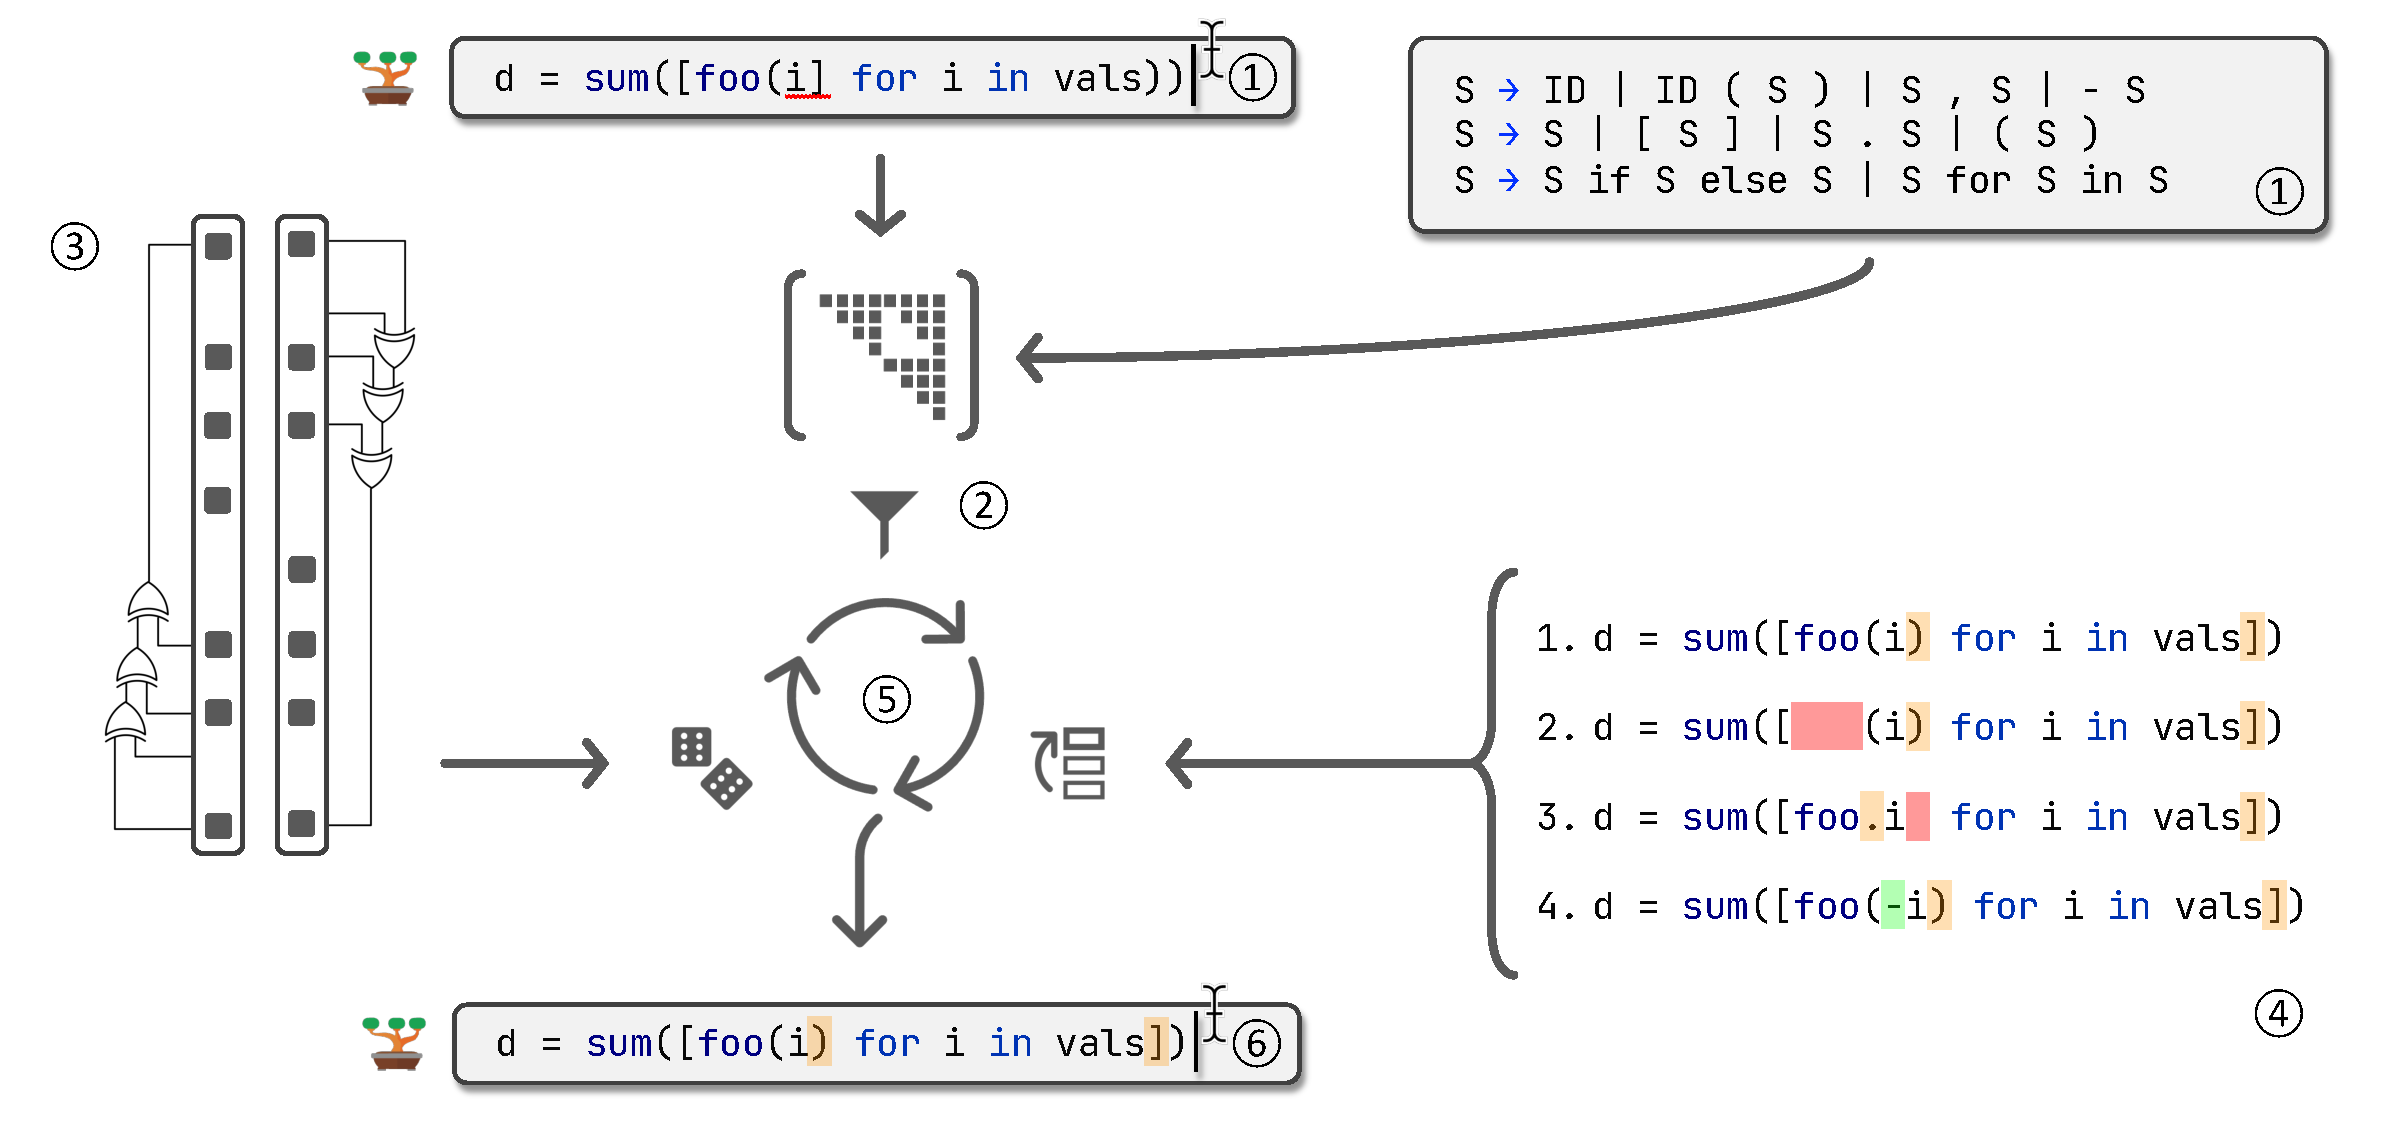
\includegraphics[width=\linewidth]{../figures/architecture_overview.pdf}
  \caption{Our framework consists of three components, namely (2) a solver, (4) ranker and (3) sampler. Given an invalid string and grammar (1), we first compile them into a Boolean tensor (2) representing a multilinear system of equations whose fixed points characterize the admissible set. The system can be solved directly, yielding a set of repairs that are ranked using a suitable scoring function (4). Optionally, we may introduce stochastic edits to the string using the Levenshtein ball sampler (3) and extract the solutions incrementally (5). When the langauge edit distance and solutions are time-sensitive, (5) is typically more efficient.}
  \label{fig:overview}
\end{figure}

Tidyparse accepts an arbitrary CFG and a string, which we first attempt to parse using Valiant's parser (\S\ref{sec:matrix}). If the string is invalid, we attempt to repair it by sampling a stochastic sequence of holes without replacement from the Levenshtein ball, then extract all valid strings. This sequence can be viewed as an elliptic curve over the set of all edits within a small neighborhood, filtered through a recognizer. Below is an example illustrating this procedure on a single Python snippet.

\begin{enumerate}
  \item \texttt{d = sum([foo(i\err{]} for i in vals))}
  \item \begin{tabular}{|c|c|c|c|c|c|c|c|c|c|c|c|c|c|c|}
          \hline
          \texttt{d} & \texttt{=} & \texttt{sum} & \texttt{(} & \texttt{[} & \texttt{foo} & \texttt{(} & \texttt{i} & \texttt{]} & \texttt{for} & \texttt{i} & \texttt{in} & \texttt{vals} & \texttt{)} & \texttt{)} \\\hline
  \end{tabular}
  \item \begin{tabular}{|c|c|c|c|c|c|c|c|c|c|c|c|c|c|c|}
          \hline
          \texttt{w} & \texttt{=} & \texttt{w} & \texttt{(} & \texttt{[} & \texttt{w} & \texttt{(} & \texttt{w} & \texttt{]} & \texttt{for} & \texttt{w} & \texttt{in} & \texttt{w} & \texttt{)} & \texttt{)} \\\hline
  \end{tabular}
  \item \begin{tabular}{|||c|||c|||c|||c|||c|||c|||c|||c|||c|||c|||c|||c|||c|||c|||c|||}
          \hline
          \texttt{w} & \texttt{=} & \texttt{w} & \texttt{(} & \texttt{[} & \texttt{w} & \texttt{(} & \texttt{w} & \texttt{]} & \texttt{for} & \texttt{w} & \texttt{in} & \texttt{w} & \texttt{)} & \texttt{)} \\\hline
  \end{tabular}
  \item \begin{tabular}{|||c|||c|||c|||c|||c|||c|||c|||c|||c|||c|||c|||c|||c|||c|||c|||}
          \hline
          \cellcolor{black!15}\texttt{\_} & \texttt{=} & \cellcolor{black!15}\texttt{\_} & \texttt{(} & \texttt{[} & \texttt{w} & \texttt{(} & \texttt{w} & \texttt{]} & \texttt{for} & \texttt{w} & \texttt{in} & \texttt{w} & \texttt{)} & \cellcolor{black!15}\texttt{\_} \\\hline
  \end{tabular}\\
  \begin{tabular}{|||c|||c|||c|||c|||c|||c|||c|||c|||c|||c|||c|||c|||c|||c|||c|||}
    \hline
    \texttt{w} & \cellcolor{black!15}\texttt{\_} & \texttt{w} & \texttt{(} & \texttt{[} & \cellcolor{black!15}\texttt{\_} & \texttt{(} & \texttt{w} & \texttt{]} & \texttt{for} & \texttt{w} & \cellcolor{black!15}\texttt{\_} & \texttt{w} & \texttt{)} & \texttt{)} \\\hline
%          \cellcolor{black!15}\texttt{\_} & \texttt{=} & \cellcolor{black!15}\texttt{\_} & \texttt{(} & \texttt{[} & \texttt{w} & \texttt{(} & \texttt{w} & \texttt{]} & \texttt{for} & \texttt{w} & \texttt{in} & \texttt{w} & \texttt{)} & \cellcolor{black!15}\texttt{\_} \\\hline
%          & & & & & & & & & & & & & & \\\hline
  \end{tabular}\\$\cdots$
  \item \begin{tabular}{|||c|||c|||c|||c|||c|||c|||c||c|c|||c|||c|||c|||c|||c|||c|||c|||}
          \hline
%          \texttt{w} & \texttt{=} & & \texttt{w} & \texttt{(} & \texttt{[} & \texttt{w} & \texttt{(} & \texttt{w} & \texttt{]} & \texttt{for} & \texttt{w} & \texttt{in} & \texttt{w} & \texttt{)} & \texttt{)} \\\hline
          \texttt{w} & \texttt{=} & \texttt{w} & \texttt{(} & \texttt{[} & \texttt{w} & \texttt{(} & \cellcolor{black!15}\texttt{\_} &  \texttt{w} & \cellcolor{black!15}\texttt{\_} & \texttt{for} & \texttt{w} & \texttt{in} & \texttt{w} & \cellcolor{black!15}\texttt{\_} & \texttt{)} \\\hline
          & & & & & & & \cellcolor{green!25}\texttt{+} & & \cellcolor{orange!25}\texttt{)} & & & & & \cellcolor{orange!25}\texttt{]} & \\\hline
  \end{tabular}
  \item (a) \texttt{d = sum([foo(\hlgreen{+}i\hlorange{)} for i in vals\hlorange{]})} $\Longrightarrow$ (b) \texttt{d = sum([foo(i\hlorange{)} for i in vals\hlorange{]})}
\end{enumerate}

The initial broken string, \texttt{d = sum([foo(i\err{]} for i in vals))} (1), is first tokenized using a lexer to obtain the sequence in (2). Lexical tokens containing identifiers are abstracted in step (3), and interleaved with the empty token in step (4). We then sample hole configurations without replacement in step (5), many of which will have no admissible solutions. Eventually, the solver will discover an admissible solution, as seen in step (6). This solution is then used to generate a patch, which is applied to the original string in step (7a), then reduced to its minimal form in step (7b), and sampling is repeated until all possibilities are exhausted or a predetermined timeout expires.

Optionally, we may bias the sampler toward previously discovered repairs by adding successful patches to a replay buffer ranked by likelihood. This buffer can then be stochastically resampled using a Dirichlet process with stepwise decaying exploration to encourage diversity. As shown in \S\ref{sec:experiments}, we found this approach to be significantly more sample-efficient with respect to language membership, yielding much higher precision and repair throughput under low-latency constraints.

Using the Levenshtein ball sampler as a proposal distribution, we then solve for the least fixpoint of an idempotent matrix to obtain the set of syntactically admissible repairs, all of which are guaranteed to be minimal and syntactically valid. These repairs are finally reranked according to their statistical likelihood, and the most likely repairs discovered within a fixed time are presented to the user. We describe our solver in more detail in \S\ref{sec:matrix} and this whole process is illustrated in Fig.~\ref{fig:overview}.

During the conception of this work, a number of design choices were made to increase its utility as a real-time programming assistant, which aims to provide precise and continuous feedback while the user is typing across a variety of programming languages. To support this use case, the following criteria were taken into account when designing and evaluating various components:

\begin{itemize}
  \item First and foremost, the framework must be \textbf{sound} and \textbf{complete}. That is, the parser-generator must (1) accept arbitrary conjunctive grammars, and (2) generate a parser which accepts all and only syntactically valid strings and (3) when a string is invalid, our synthesizer must eventually generate every syntactically valid string within a fixed distance from it.
  \item Second, we require that the resulting repairs be \textbf{plausible} and \textbf{diverse}. In other words, the framework should generate repairs that are likely to be written by a human being, consistent with the surrounding context, and reasonably diverse in their structure.
  \item Third, the framework must be \textbf{efficient} and \textbf{responsive}. That is, it must be able to recognize well-formed strings in subcubic time, and generate admissible repairs in subpolynomial time. These conditions are necessary to provide real-time feedback whilst the user is typing.
  \item Fourth, the framework must also be \textbf{robust} and \textbf{scalable}. In practice, this means that the framework should be robust to multiple errors, handle grammars with a large number of productions and be able to scale linearly as the number of processor cores are increased.
  \item Finally, the framework must be \textbf{flexible} and \textbf{extensible}. Intended as a general-purpose tool for generating syntax repairs in a wide variety of programming languages, end-users should be able to extend the framework with their own custom grammars and side-constraints.
\end{itemize}

As we demonstrate both formally and experimentally, our framework is able to satisfy most of these criteria simultaneously, while attaining state-of-the-art performance in terms of precision, throughput and wall clock latency. However, there are still some open problems that remain to be solved to realize its full potential as an everyday programming tool. In particular, we will discuss some of those open problems (e.g.,~\ref{def:isolation}) and design trade-offs (\S\ref{sec:discussion}) that were taken in its construction.

With the above criteria in mind, the following paper addresses four primary research questions:

\begin{enumerate}
  \item \textbf{What theoretical guarantees do we offer?} (i.e., complexity, soundness and completeness)
  \item \textbf{How do we reduce syntax repair onto finite fields?} (i.e., algorithms and data structures)
  \item \textbf{How does Tidyparse compare with existing approaches?} (i.e., neural program repair)
  \item \textbf{What are the limitations of this technique?} (i.e., precision, latency and error tolerance)
\end{enumerate}

We will begin by precisely defining the Levenshtein-CFL reachability problem (\S\ref{sec:problem}), then construct an algebraic theory of syntax correction (\S\ref{sec:matrix}), followed by a corollary description of the parsing algorithm (\S\ref{sec:parsing}). After presenting some practical examples of the tool's features (\S\ref{sec:examples}) and taking a short detour into the related literature on syntax repair (\S\ref{sec:related}), we will then empirically evaluate the end-to-end performance on a dataset of human syntax errors and repairs (\S\ref{sec:experiments}). Finally, we will discuss the results (\S\ref{sec:discussion}) and conclude with a summary of our contributions and future work (\S\ref{sec:conclusion}).

\section{Problem statement}\label{sec:problem}

The problem of syntax error correction under a finite number of typographic errors is reducible to the bounded Levenshtein-CFL reachability problem, which can be formally stated as follows:

\begin{definition}
  The language edit distance (LED) is the minimum number of edits required to transform an invalid string into a valid one, where validity is defined as containment in a context-free language, $\ell: \mathcal{L}$, i.e., $\Delta^*(\err{\sigma}, \ell) \coloneqq \min_{\sigma \in \ell}\Delta(\err{\sigma}, \sigma)$, and $\Delta$ is the Levenshtein distance.
\end{definition}

We seek to find the set of strings $S$ such that $\forall \tilde{\sigma}\in S, \Delta(\err{\sigma}, \tilde{\sigma}) \leq q$, where $q$ is the maximum number of edits greater than or equal to the language edit distance. We call this set the \textit{Levenshtein ball} of $\err{\sigma}$ and denote it $\Delta_q(\err{\sigma})$. Since $1 \leq \Delta^*(\err{\sigma}, \ell) \leq q$, we have $1 \leq q$. We now consider an upper bound on $\Delta^*(\err{\sigma}, \ell)$, i.e., the greatest lower bound on $q$ such that $\Delta_q(\err{\sigma}) \cap \ell \neq \varnothing$.

\begin{lemma}\label{lemma:upper-bound}
  For any nonempty language $\ell: \mathcal{L}$ and invalid string $\err{\sigma}: \Sigma^n \cap \bar\ell$, there exists an $(\tilde{\sigma}, m)$ such that $\tilde{\sigma} \in \ell\cap\Sigma^m$ and $0 < \Delta(\err{\sigma}, \ell) \leq \max(m, n) < \infty$.
\end{lemma}

\begin{proof}
  Since $\ell$ is nonempty, it must have at least one inhabitant $\sigma \in \ell$. Let $\tilde{\sigma}$ be the smallest such member. Since $\tilde{\sigma}$ is a valid sentence in $\ell$, by definition it must be that $|\tilde{\sigma}|<\infty$. Let $m\coloneqq|\tilde{\sigma}|$. Since we know $\err{\sigma} \notin \ell$, it follows that $0 < \Delta(\err{\sigma}, \ell)$. Let us consider two cases, either $\tilde{\sigma} = \varepsilon$, or $0 < |\tilde{\sigma}|$:

  \begin{itemize}
    \item If $\tilde{\sigma} = \varepsilon$, then $\Delta(\err{\sigma}, \tilde{\sigma}) = n$ by full erasure of $\err{\sigma}$, or
    \item If $0 < m$, then $\Delta(\err{\sigma}, \tilde{\sigma}) \leq \max(m, n)$ by overwriting.
  \end{itemize}

  In either case, it follows $\Delta(\err{\sigma}, \ell) \leq \max(m, n)$ and $\ell$ is always reachable via a finite nonempty set of Levenshtein edits, i.e., $0 < \Delta(\err{\sigma}, \ell) < \infty$.
\end{proof}

Let us now consider the maximum growth rate of the \textit{admissible set}, $A \coloneq \Delta_q(\err{\sigma}) \cap \ell$, as a function of $q$ and $n$. Let $\bar\ell \coloneq \{\err{\sigma}\}$. Since $\bar\ell$ is finite and thus regular, $\ell = \Sigma^* \setminus \{\err{\sigma}\}$ is regular by the closure of regular languages under complementation, and thus context-free a fortiori. Since $\ell$ accepts every string except $\err{\sigma}$, it represents the worst CFL in terms of asymptotic growth of $A$.

\begin{lemma}\label{lemma:interleaving}
  The complexity of searching $A$ is upper bounded by $\mathcal{O}\left(\sum_{c=1}^q{{cn + n + 1} \choose c}(|\Sigma| + 1)^c\right)$.
\end{lemma}

\begin{proof}
  We can overestimate the size of $A$ by considering the number of unique ways to insert, delete, or substitute $c$ terminals into a string $\err{\sigma}$ of length $n$. This can be overaproximated by interleaving $\varepsilon^c$ around every token, i.e., $\err{\sigma}_\varepsilon\coloneq \left(\varepsilon^c\err{\sigma}_i\right)_{i=1}^n\varepsilon^c$, where $|\err{\sigma}_\varepsilon| = cn + n + 1$, and only considering substitution. We augment $\Sigma_\varepsilon \coloneq \Sigma \cup \{\varepsilon\}$ so that deletions and insertions may be treated as special cases of substitution. Thus, we have $cn + n + 1$ positions to substitute $(|\Sigma_\varepsilon|)$ tokens, i.e., ${{cn + n + 1} \choose c}|\Sigma_\varepsilon|^c$ ways to edit $\err{\sigma}_\varepsilon$ for each $c \in [1, q]$. This upper bound is not tight, as overcounts many identical edits w.r.t. $\err{\sigma}$. Nonetheless, it is sufficient to show $|A| < \sum_{c=1}^q{{cn + n + 1} \choose c}|\Sigma_\varepsilon|^c$.
\end{proof}

We note that the above bound applies to all strings and languages, and relates to the Hamming bound on $H_q(\err{\sigma}_\varepsilon)$, which only considers substitutions.~\footnote{This reflects our general approach, which builds a surjection from the interleaved Hamming ball onto the Levenshtein ball.} In practice, much tighter bounds may be obtained by considering the structure of $\ell$ and $\err{\sigma}$. For example, based on an empirical evaluation from a dataset of human errors and repairs in Python code snippets ($|\Sigma| = 50, |\err{\sigma}| < 40, \Delta(\err{\sigma}, \ell) \in [1, 3]$), we estimate the \textit{filtration rate}, i.e., the density of the admissible set relative to the Levenshtein ball, $D=|A|/|\Delta_q(\err{\sigma})|$ to have empirical mean $E_\sigma[D] \approx 2.6\times 10^{-4}$, and variance $\mathrm{Var}_\sigma[D] \approx 3.8\times10^{-7}$.

In practice, this problem is ill-posed even when $q = \Delta^*(\err{\sigma}, \ell) \approx 1$. For example, consider the language of ursine dietary preferences. Although $\err{\sigma}\coloneq$ ``Bears like to eat plastic'' is not a valid sentence, e.g., $\tilde{\sigma}\coloneq$``Bears like to eat'' is $(\Delta^*=1)$, however there are many others with roughly the same edit distance, e.g., ``Bears like to eat \{\hlorange{berries}, \hlorange{honey}, \hlorange{fish}\}'', or ``\{\hlgreen{Polar}, \hlgreen{Panda}\} bears like to eat \{\hlgreen{seals}, \hlgreen{bamboo}\}''. In general, there are usually many strings nearby $\err{\sigma}$, and we seek to find those among them which are both syntactically valid and semantically plausible as quickly as possible.

\section{Matrix Theory}\label{sec:matrix}

Recall that a CFG is a quadruple consisting of terminals $(\Sigma)$, nonterminals $(V)$, productions $(P\colon V \rightarrow (V \mid \Sigma)^*)$, and a start symbol, $(S)$. It is a well-known fact that every CFG is reducible to \textit{Chomsky Normal Form}, $P'\colon V \rightarrow (V^2 \mid \Sigma)$, in which every production takes one of two forms, either $w \rightarrow xz$, or $w \rightarrow t$, where $w, x, z: V$ and $t: \Sigma$. For example:\vspace{-3pt}

\begin{table}[H]
\begin{tabular}{llll}
$\mathcal{G}\coloneqq\big\{\;S \rightarrow S\:S \mid (\:S\:) \mid (\:)\;\big\} \Longrightarrow \mathcal{G}'=\big\{\;S\rightarrow Q\:R \mid S\:S \mid L\:R,$ & $R \rightarrow\:),$ & $L \rightarrow (,$ & $Q\rightarrow L\:S\;\big\}$
\end{tabular}
\end{table}\vspace{-8pt}

\noindent Given a CFG, $\mathcal{G}' : \mathbb{G} = \langle \Sigma, V, P, S\rangle$ in CNF, we can construct a recognizer $R: \mathbb{G} \rightarrow \Sigma^n \rightarrow \mathbb{B}$ for strings $\sigma: \Sigma^n$ as follows. Let $2^V$ be our domain, $0$ be $\varnothing$, $\oplus$ be $\cup$, and $\otimes$ be defined as:\vspace{-10pt}

\begin{align}
X \otimes Z \coloneqq \big\{\;w \mid \langle x, z\rangle \in X \times Z, (w\rightarrow xz) \in P\;\big\}
\end{align}

\noindent If we define $\sigma_r^{\shur} \coloneqq \{w \mid (w \rightarrow \sigma_r) \in P\}$, then construct a matrix with nonterminals on the superdiagonal representing each token, $M^0_{r+1=c}(\mathcal{G}', e) \coloneqq \;\sigma_r^{\shur}$ and solve for the fixpoint $M^* = M + M^2$,\vspace{-10pt}

\begin{align*}
M^0\coloneqq
\begin{pNiceMatrix}[nullify-dots,xdots/line-style=loosely dotted]
   \varnothing & \sigma_1^\shri & \varnothing & \Cdots & \varnothing \\
   \Vdots      & \Ddots         & \Ddots      & \Ddots & \Vdots\\
               &                &             &        & \varnothing\\
               &                &             &        & \sigma_n^\shup \\
   \varnothing & \Cdots         &             &        & \varnothing
\end{pNiceMatrix} &\Rightarrow
\begin{pNiceMatrix}[nullify-dots,xdots/line-style=loosely dotted]
  \varnothing & \sigma_1^\shri & \Lambda & \Cdots & \varnothing \\
  \Vdots      & \Ddots         & \Ddots  & \Ddots & \Vdots\\
              &                &         &        & \Lambda\\
              &                &         &        & \sigma_n^\shup \\
  \varnothing & \Cdots         &         &        & \varnothing
\end{pNiceMatrix} &\Rightarrow \ldots \Rightarrow M^* =
\begin{pNiceMatrix}[nullify-dots,xdots/line-style=loosely dotted]
   \varnothing & \sigma_1^\shri & \Lambda & \Cdots & \Lambda^*_\sigma\\
   \Vdots      & \Ddots         & \Ddots  & \Ddots & \Vdots\\
               &                &         &        & \Lambda\\
               &                &         &        & \sigma_n^\shup \\
   \varnothing & \Cdots         &         &        & \varnothing
\end{pNiceMatrix}
\end{align*}

\noindent we obtain the recognizer, $R(\mathcal{G}', \sigma) \coloneqq [S \in \Lambda^*_\sigma] \Leftrightarrow [\sigma \in \mathcal{L}(\mathcal{G})]$~\footnote{Hereinafter, we use Iverson brackets to denote the indicator function of a predicate with free variables, i.e., $[P] \Leftrightarrow \mathds{1}(P)$.}.

Since $\bigoplus_{c = 1}^n M_{r,c} \otimes M_{c,r}$ has cardinality bounded by $|V|$, it can be represented as $\mathbb{Z}_2^{|V|}$ using the characteristic function, $\mathds{1}$. Note that any encoding which respects linearity $\varphi(\Lambda \circledast \Lambda') \equiv \varphi(\Lambda) \circledast \varphi(\Lambda')$ is suitable -- this particular representation shares the same algebraic structure, but is more widely studied in error correction, and readily compiled into circuits and BLAS primitives. Furthermore, it enjoys the benefit of complexity-theoretic speedups to matrix multiplication.

Details of the bisimilarity between parsing and matrix multiplication can be found in Valiant~\cite{valiant1975general}, who first realized its time complexity was subcubic $\mathcal{O}(n^\omega)$ where $\omega$ is the asymptotic lower bound for Boolean matrix multiplication ($\omega < 2.77$), and Lee~\cite{lee2002fast}, who shows that speedups to CFL parsing were realizable by Boolean matrix multiplication algorithms. While more efficient specialized parsers are known to exist for restricted CFGs, this technique is typically lineararithmic under sparsity and believed to be the most efficient general procedure for CFL parsing.

\subsection{Parsing with holes}

Valiant's algorithm can be abstracted by lifting it into the domain of linear equations over finite fields, where each bitvector in the upper triangular matrix instead contains polynomials whose solutions identify nonterminals participating in the parse forest of a \textit{porous string} on the superdiagonal (our work). This interpretation of Valiant's algorithm as an equational theory offers a novel polynomial reduction from language equations onto XORSAT. More formally, we solve the following problem:% e.g., langauge membership, langauge quotient, and reachability

\begin{definition}[Hole subsumption]
  Let $\underline\Sigma \coloneqq \Sigma \cup \{\_\}$, where $\_$ represents a hole. We denote $\sqsubseteq: \underline\Sigma^n \times \Sigma^n$ as the relation $\{\langle\sigma, \sigma'\rangle \mid \sigma_i \in \Sigma \implies \sigma_i = \sigma_i'\}$ and the set of all $\{\sigma' \mid \sigma' \sqsubseteq \sigma\}$ as $\text{H}(\sigma)$.
\end{definition}

\begin{definition}[Parsing with holes]
Let $\underline\Sigma \coloneq \Sigma \cup \{\_\}$, where holes denote free variables over $\Sigma$. Given a CFG, $\mathcal{G}: \mathbb{G}$, and a \textit{porous string}, $\sigma: \underline\Sigma^{n-1}, n: \mathbb{N}^{\geq 3}$, let us define $A(\sigma, \mathcal{G})\coloneqq\text{H}(\sigma)\cap\mathcal{L}(\mathcal{G})$. We can extract $A(\sigma, \mathcal{G})$ by encoding $\langle\sigma, \mathcal{G}\rangle$ as an idempotent matrix, $\mathcal{M}_\sigma\coloneqq (\mathbb{Z}_2^{|V|}\rightarrow\mathbb{Z}_2^{|V|})^{n \times n}$, and solving for all fixedpoints $[\mathcal{M}_\sigma = \mathcal{M}_\sigma^2]$, whose models are then decoded into $\sigma' \in A(\sigma, \mathcal{G})$.
\end{definition}

\noindent The precise encoding is immaterial, as long as $\langle\boxplus, \boxtimes\rangle$ are defined so the diagram below commutes,\footnote{Hereinafter, we use gray highlighting to denote types and functions defined over strings and binary constants only.}

\begin{figure}[H]
  \adjustbox{center}{%
    \[\begin{tikzcd}[row sep=large, column sep=huge]
        \langle\mathcal{G}', \highlight{\Sigma}^{n-1}\rangle \arrow[leftrightarrow, drrr, shorten=-1mm] & & [-135pt] & \vspace{20pt}\stackrel{\text{(Parsing)}}{\text{Set}} \arrow[d, phantom] & \stackrel{\text{(Recognition)}}{\text{Bit}} \arrow[d, phantom] & [-90pt] & \langle\mathcal{G}', \underline\Sigma^{n-1}\rangle \arrow[drr, shorten=-2mm] & [-90pt] & \stackrel{\text{(Synthesis)}}{\text{SAT}} \arrow[d, phantom]\\[-30pt]
        \text{Rubix}  \arrow[rr, phantom] & & [-135pt] & M \times M \arrow[r, "\mathds{1}^{2^{n\times n}}", labels=above] \arrow[d, "\hspace{-13pt}\bigoplus\:\bigotimes"] & \mathbb{Z}_2^{|V|^{n\times n}} \times \mathbb{Z}_2^{|V|^{n\times n}} \arrow[d, "\hspace{-13.4pt}\highlight{+}\:\highlight{*}"] \arrow[l, "\mathds{1}^{-2^{n\times n}}", labels=below] \arrow[rrrr, rightarrowtail, "\varphi^{2^{n\times n}}", labels=above] & [-90pt] & & [-90pt] & \mathcal{M} \times \mathcal{M} \arrow[llll, rightharpoonup, shorten=1mm, "\varphi^{-2^{n\times n}}", labels=below] \arrow[d, "\hspace{-9pt}+\:\:\:*"] \\
        \text{Matrix} \arrow[rr, phantom] & & [-135pt] & 2^V \times 2^V \arrow[r, "\mathds{1}^{2}", labels=above] \arrow[d, "\hspace{-9pt}\oplus\:\otimes"] & \mathbb{Z}_2^{|V|} \times \mathbb{Z}_2^{|V|} \arrow[d, "\hspace{-15.8pt}\highlight{\boxplus}\:\highlight{\boxtimes}"] \arrow[l, "\mathds{1}^{-2}", labels=below] \arrow[rrrr, rightarrowtail, "\varphi^2", labels=above] & [-90pt] & & [-90pt] & \mathcal{V} \times \mathcal{V} \arrow[llll, rightharpoonup, shorten=1mm, "\varphi^{-2}", labels=below] \arrow[d, "\hspace{-9.5pt}\boxplus\:\boxtimes"] \arrow[u] \\
        \text{Vector} \arrow[rr, phantom] & & [-135pt] & 2^V \arrow[r, "\mathds{1}", labels=above] & \mathbb{Z}_2^{|V|} \arrow[l, "\mathds{1}^{-1}", labels=below] \arrow[rrrr, rightarrowtail, "\varphi", labels=above] & [-90pt] & & [-90pt] & \mathcal{V} \arrow[llll, rightharpoonup, shorten=1mm, "\varphi^{-1}", labels=below] \arrow[u]
    \end{tikzcd}\]
  }
\end{figure}

\noindent where $\mathcal{V}$ is a function $\mathbb{Z}_2^{|V|}\rightarrow\mathbb{Z}_2$. Note that while always possible to encode $\mathbb{Z}_2^{|V|} \rightarrow \mathcal{V}$ using the identity function, an arbitrary $\mathcal{V}$ might have zero, one, or in general, multiple solutions in $\mathbb{Z}_2^{|V|}$. In practice, this means that a language equation can be unsatisfiable or underconstrained, however if a solution exists, it can always be decoded into a valid sentence in the language $\mathcal{L}(\mathcal{G})$.

So far, we have only considered the syntactic theory of breadth-bounded CFLs with holes, however, our construction can be easily extended to handle the family of CFLs closed under conjunction. The additional expressivity afforded by the language conjunction will be indispensable when considering more practical program repair scenarios that may not be context-free.

\subsection{Linear conjunctive reachability}\label{sec:lclreach}

While generally quite expressive, CFLs are themselves not closed under intersection and have other practical limitations, i.e., are unable to express indentation or variable binding. These limitations motivate us toward more expressive yet still efficiently parsable formalisms. In the case of intersection, let us consider the traditional example, $\mathcal{L}_\cap \coloneqq \mathcal{L}(\mathcal{G}_1) \cap \mathcal{L}(\mathcal{G}_2)$ defined as follows:

\begin{table}[H]
  \begin{tabular}{llll}
    $P_1 \coloneqq \big\{\;S \rightarrow L\:R,$ & $\:L \rightarrow a\:b \mid a\:L\:b,$ & $R \rightarrow c \mid c \:R\;\big\}$\vspace{5pt}\\
    $P_2 \coloneqq \big\{\;S \rightarrow L\:R,$ & $\:R \rightarrow b\:c \mid b\:R\:c,$ & $L \rightarrow a \mid a \:L\;\big\}$
  \end{tabular}
\end{table}

\noindent Note that $\mathcal{L}_\cap$ generates the language $\big\{\;a^d b^d c^d \mid d > 0\;\big\}$, which according to the pumping lemma is not context-free. However, we can encode the intersection between two or more languages as a single SAT formula by representing  each upper-triangular matrix $\bigcap_{i=1}^c \mathcal{L}(\mathcal{G}_i)$ as a polygonal prism with upper-triangular matrices adjoined to each rectangular face. More precisely, we intersect all terminals $\Sigma_\cap \coloneqq \bigcap_{i=1}^c \Sigma_i$, then for each $t_\cap \in \Sigma_\cap$ and CFG, construct an equivalence class $E(t_\cap, \mathcal{G}_i) = \{ w_i \mid (w_i \rightarrow t_\cap) \in P_i\}$ and bind them together using conjunction:\vspace{-5pt}

\begin{align}
  \bigwedge_{t\in\Sigma_\cap}\bigwedge_{j = 1}^{c-1}\bigwedge_{i=1}^{|\sigma|} E(t_{\cap}, \mathcal{G}_j) \equiv_{\sigma_i} E(t_{\cap}, \mathcal{G}_{j+1})
\end{align}
% Generated by cfl4_intersection.vox, open with https://voxelator.com/
\begin{figure}[H]
  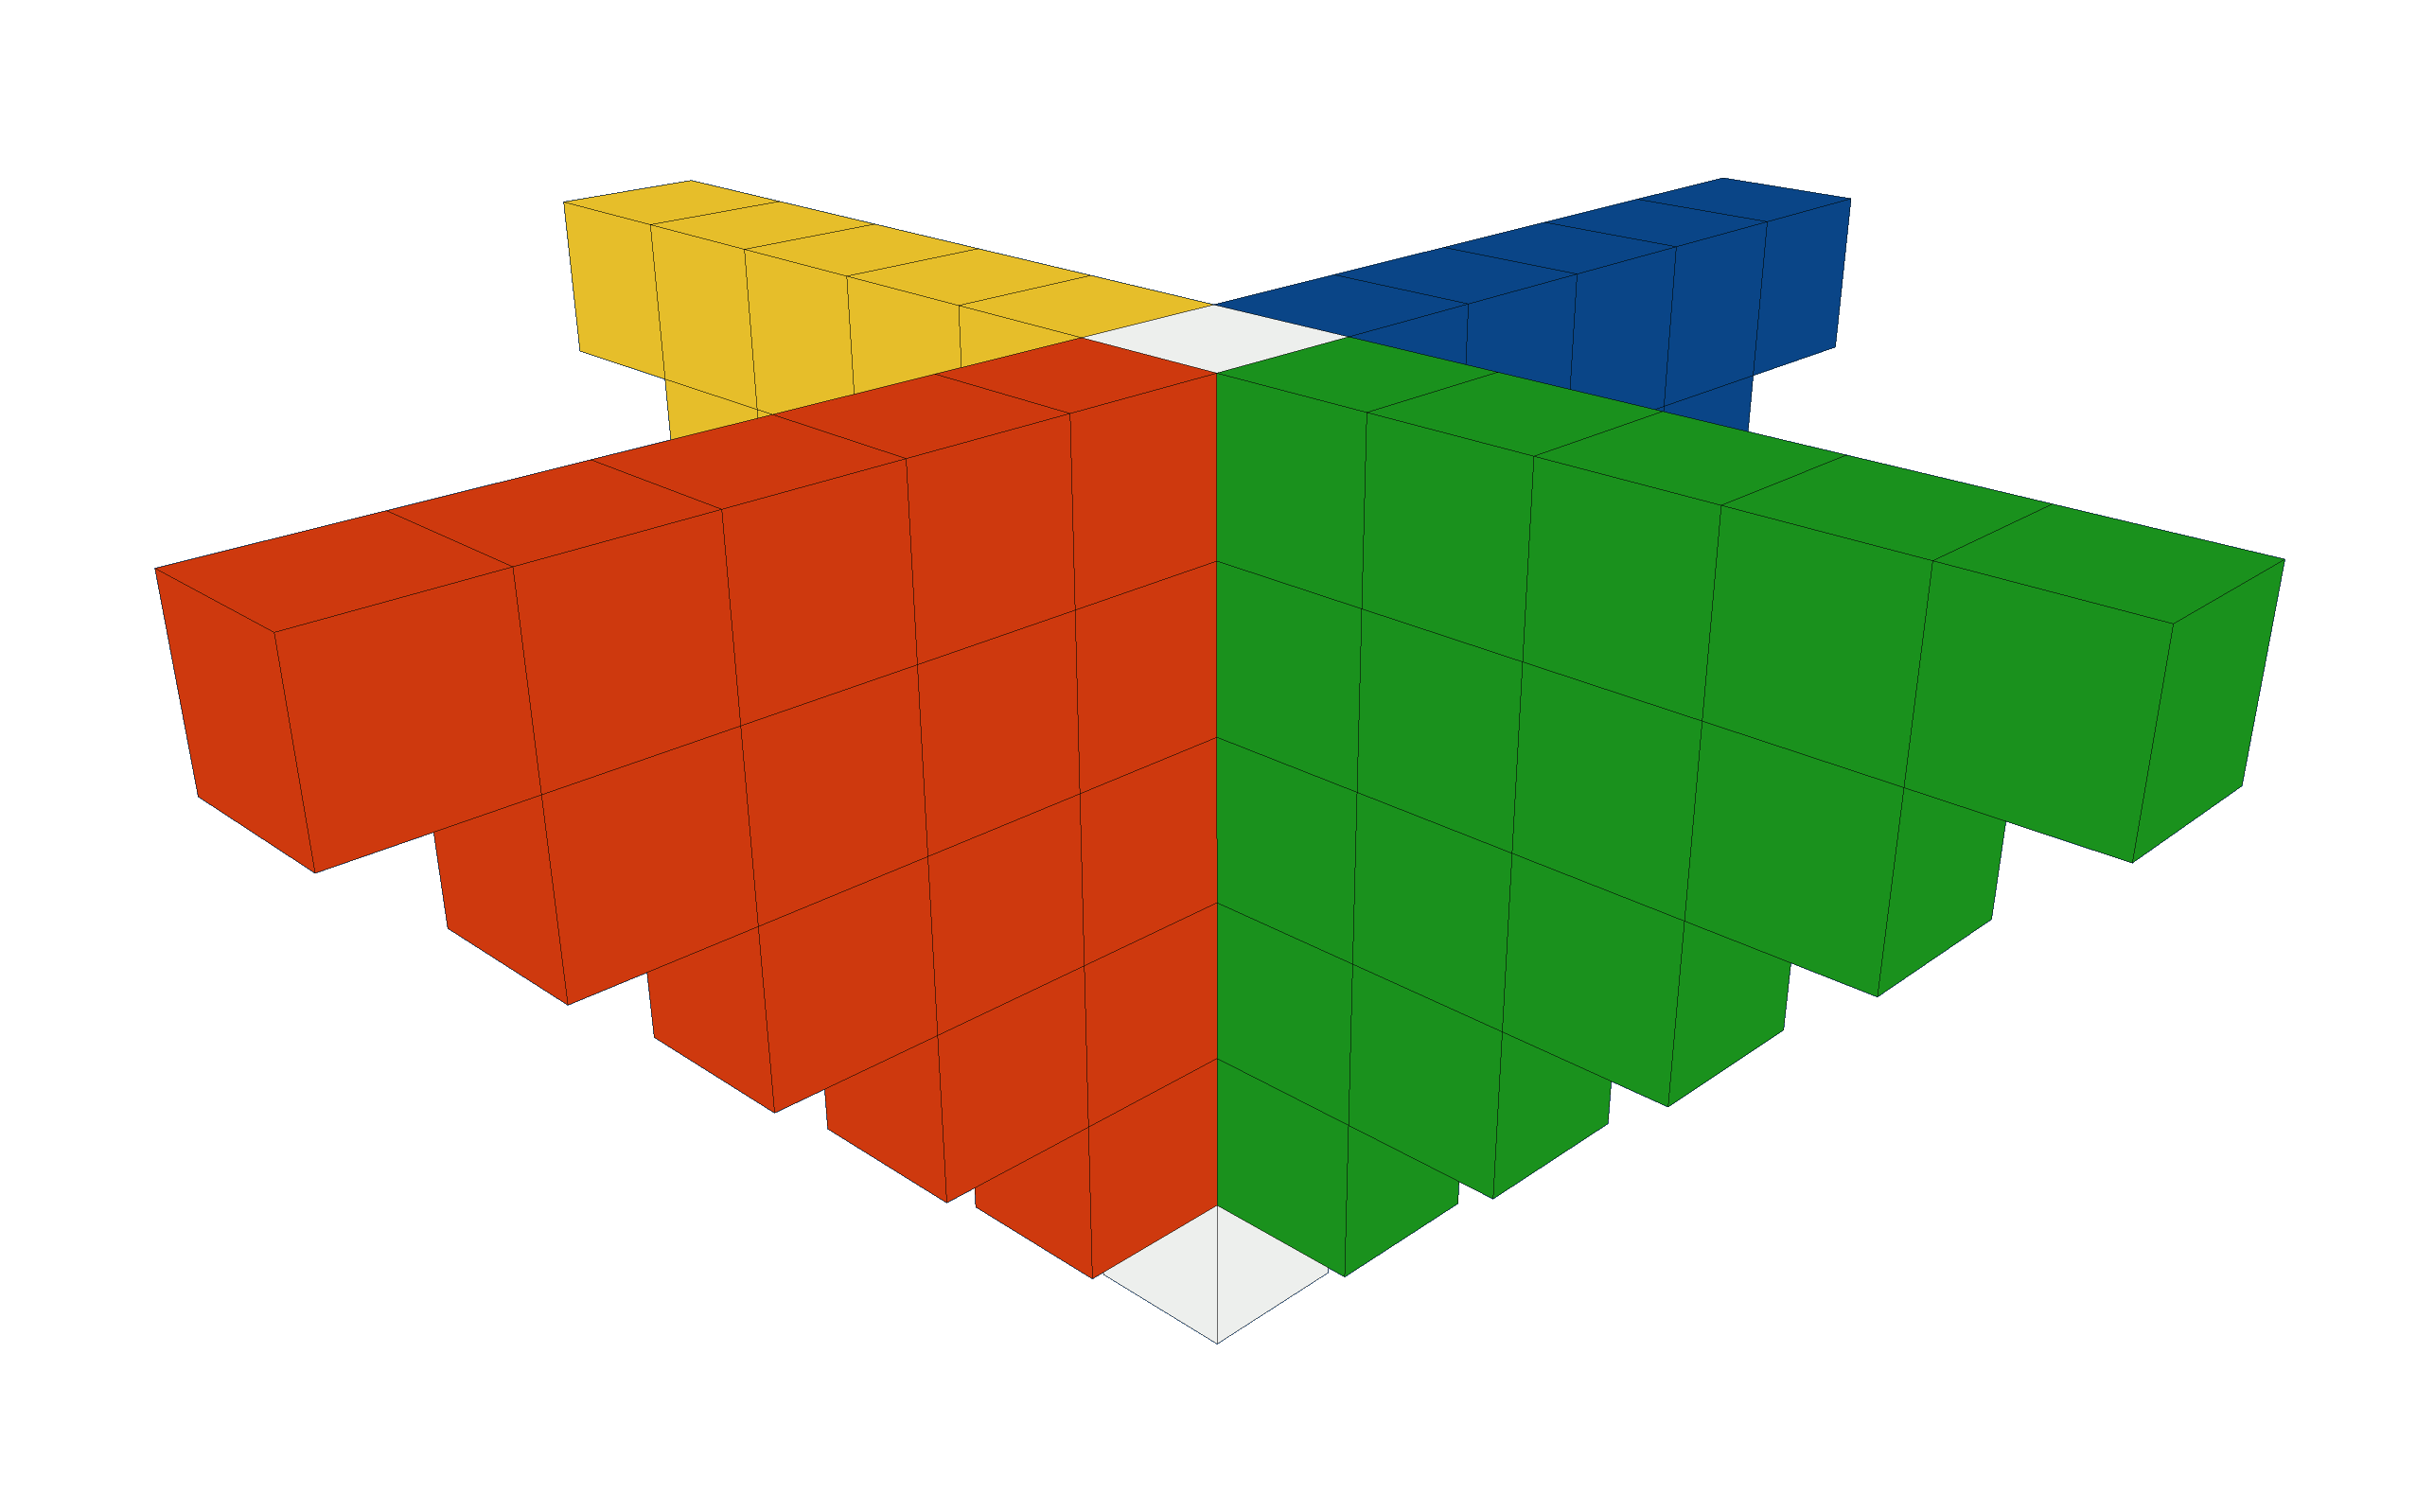
\includegraphics[height=0.1\textwidth]{../figures/angle1.png}\hspace{-5pt}
  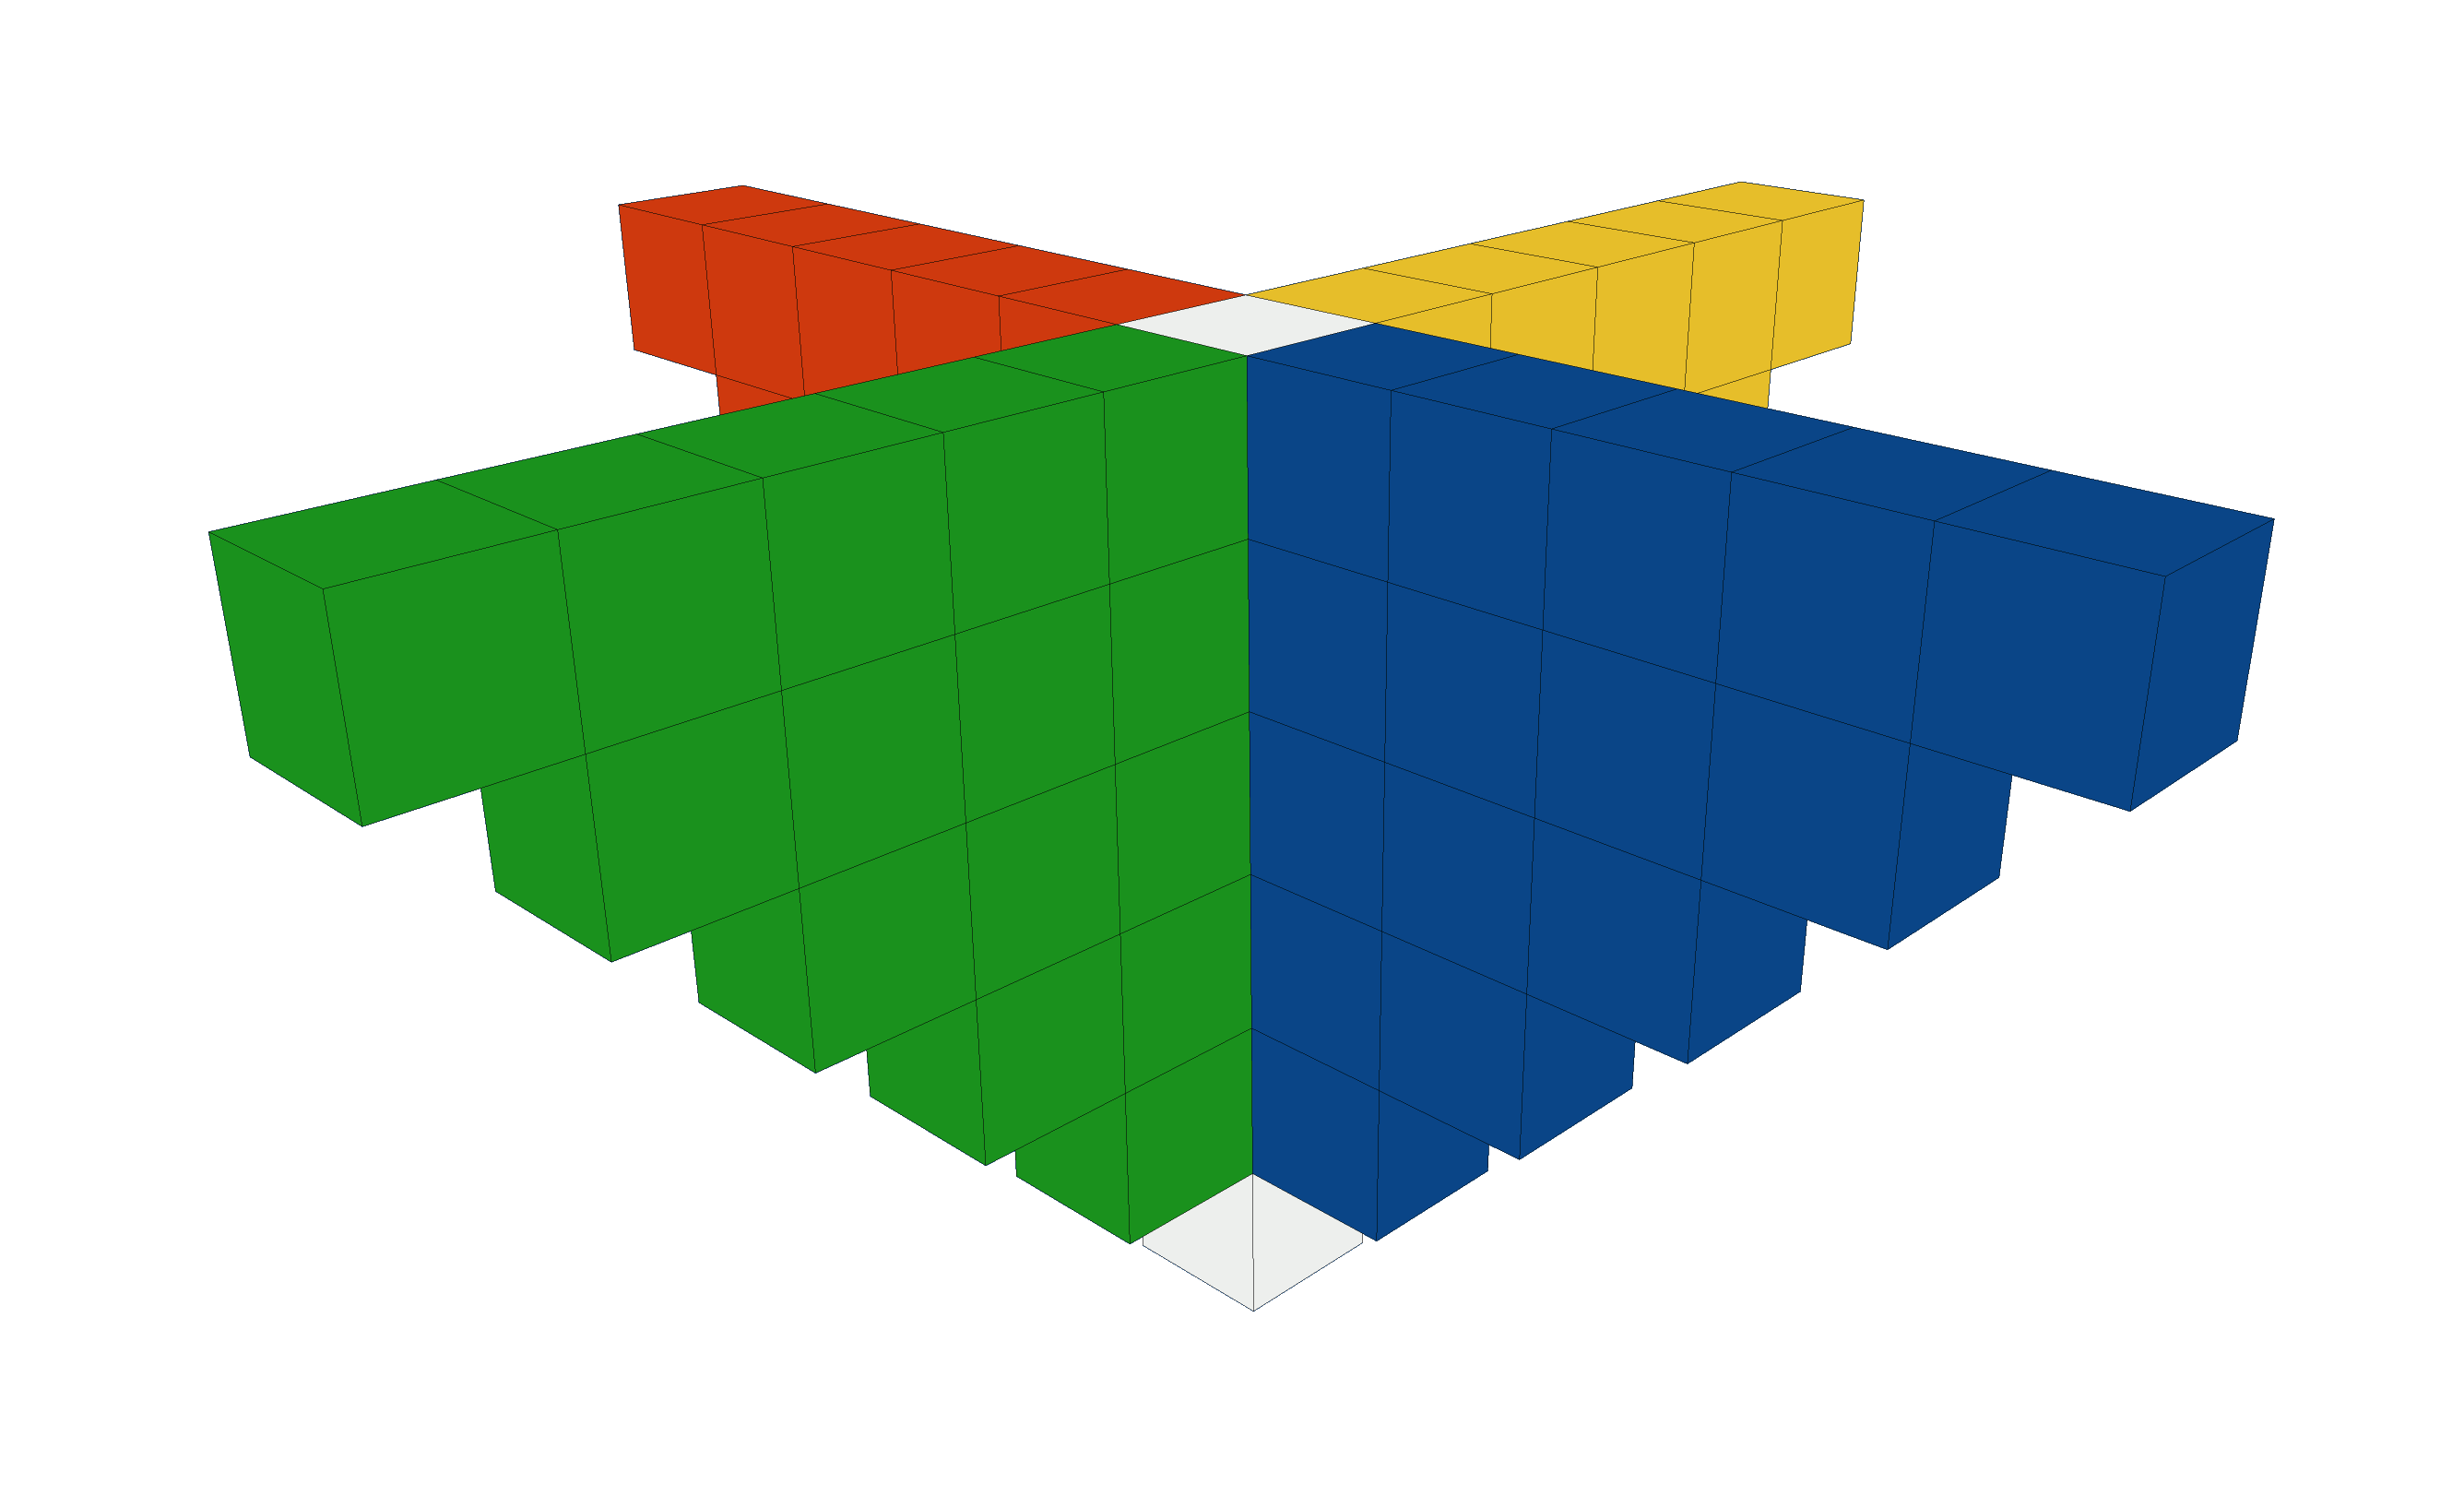
\includegraphics[height=0.1\textwidth]{../figures/angle2.png}\hspace{-5pt}
  
\includegraphics[height=0.1\textwidth]{../figures/angle5.png}\hspace{-5pt}
  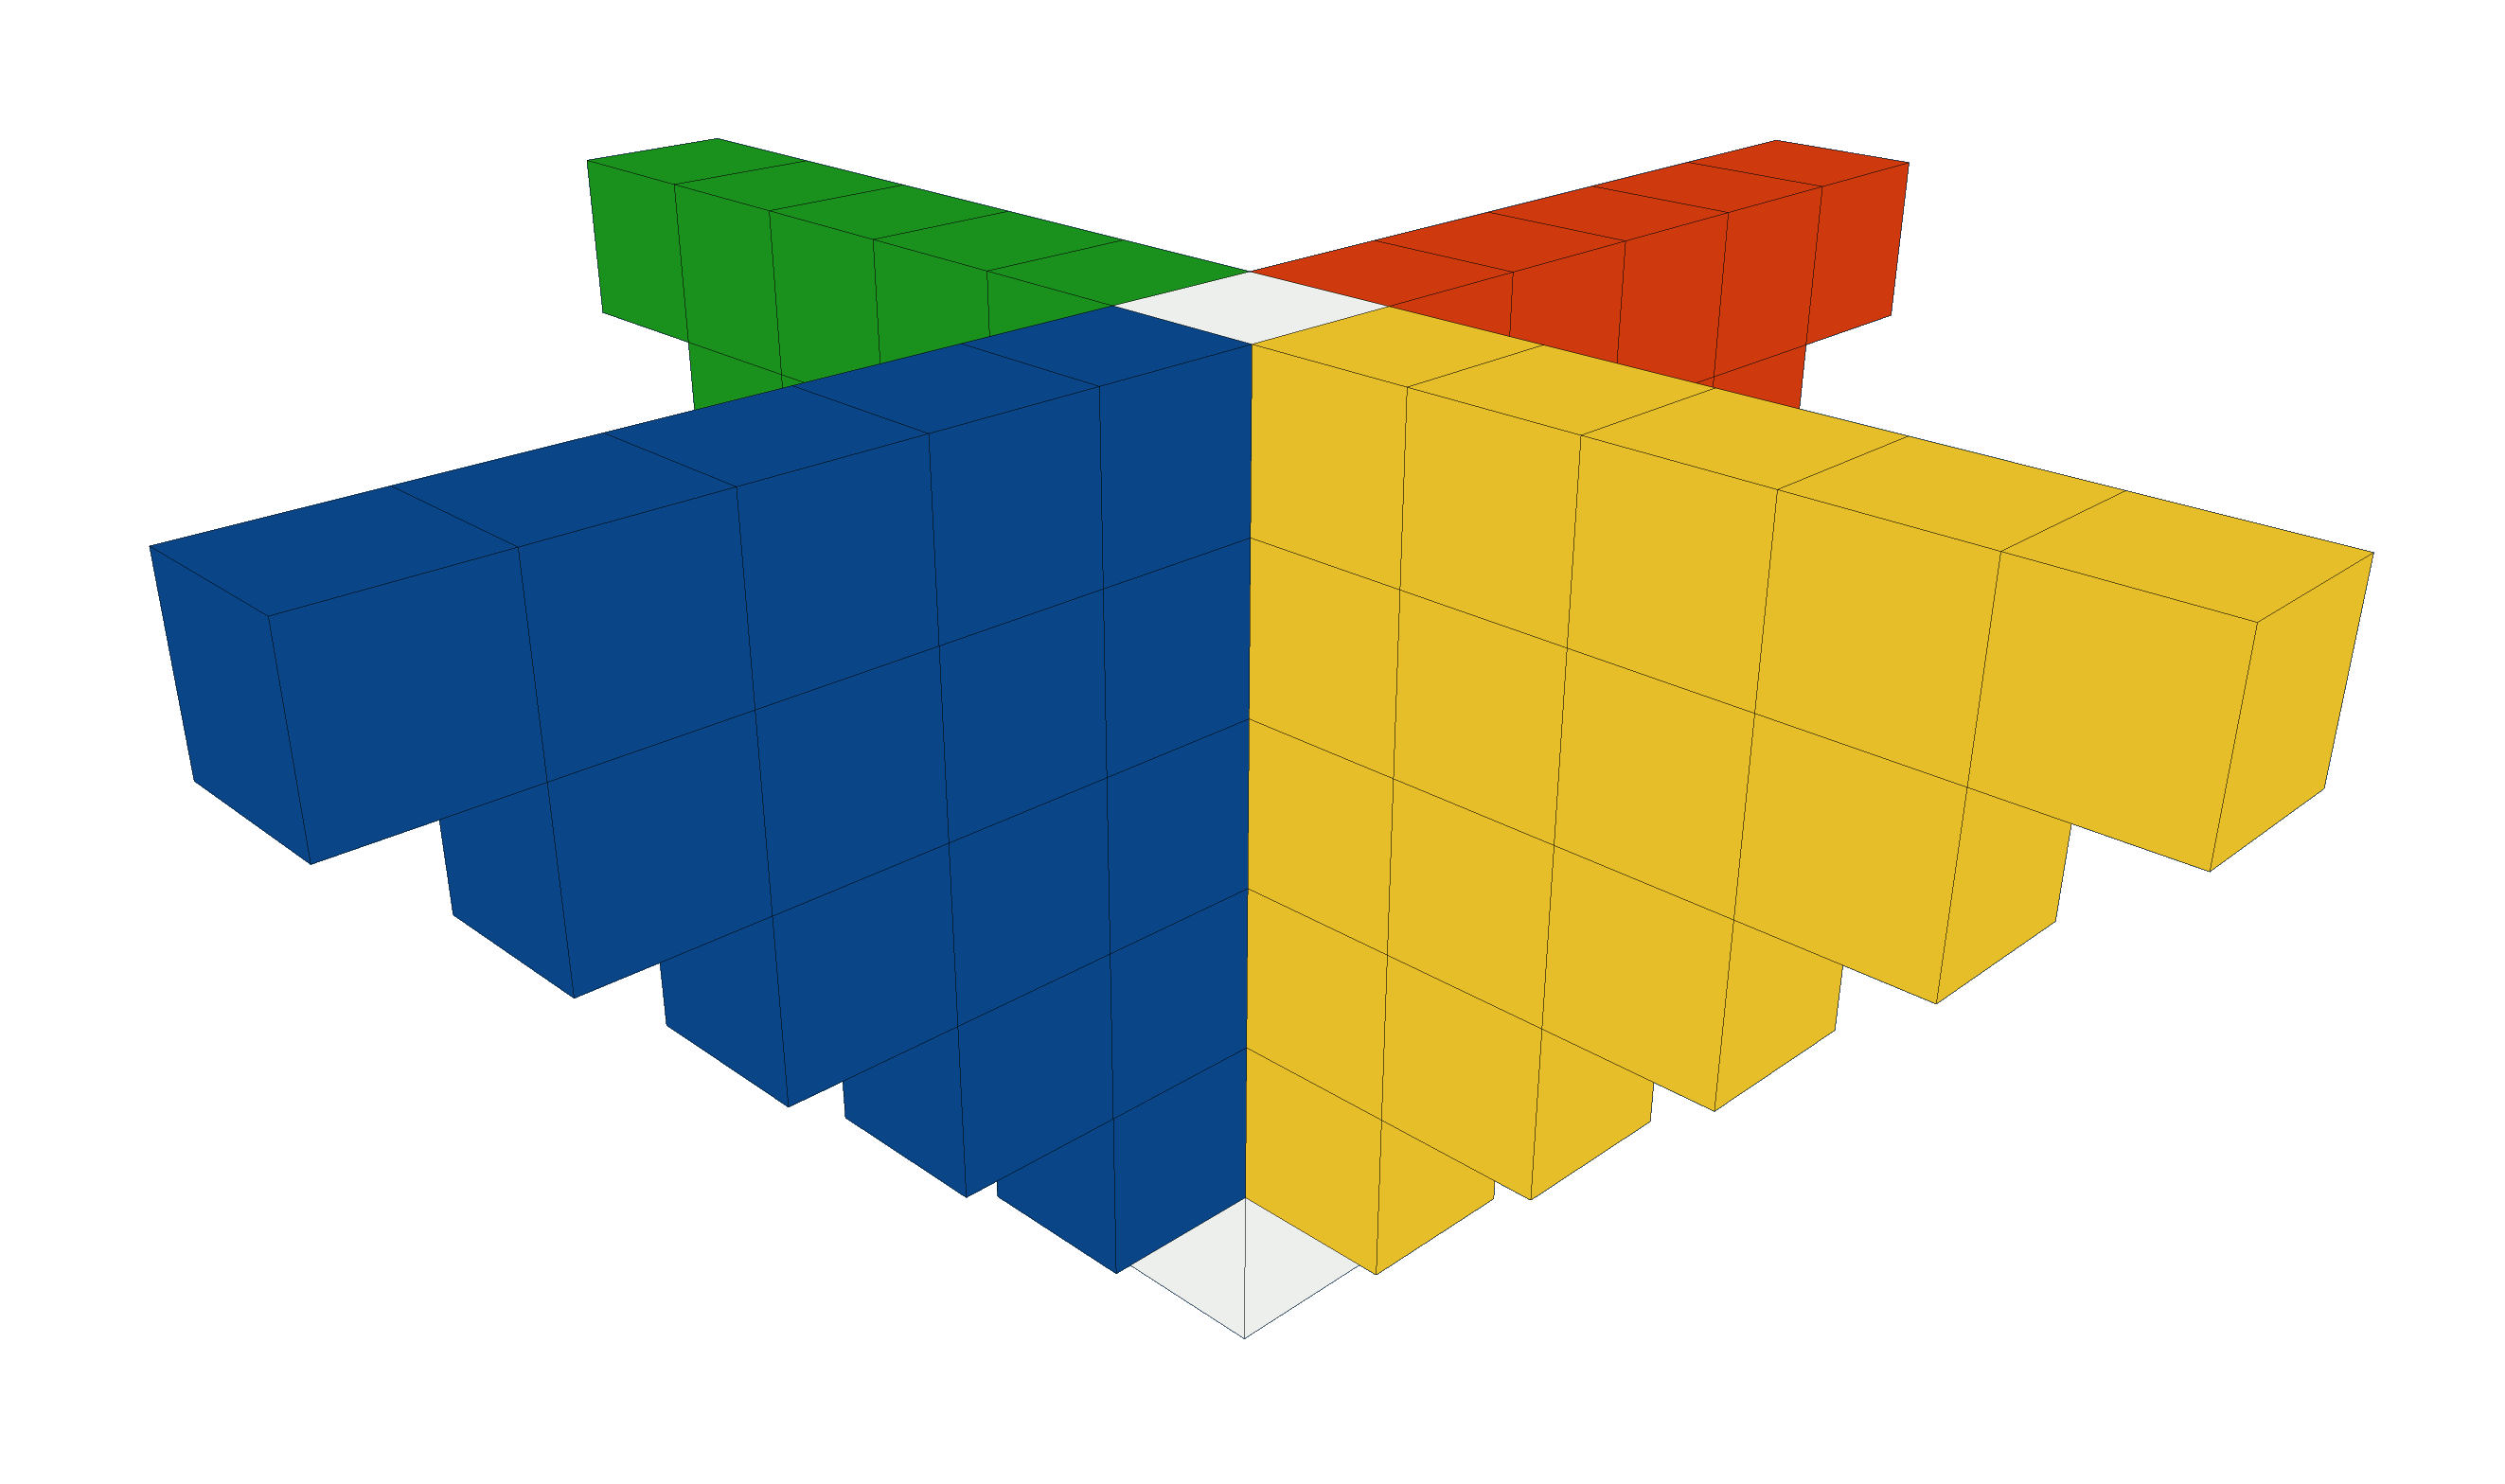
\includegraphics[height=0.1\textwidth]{../figures/angle3.png}\hspace{-3pt}
  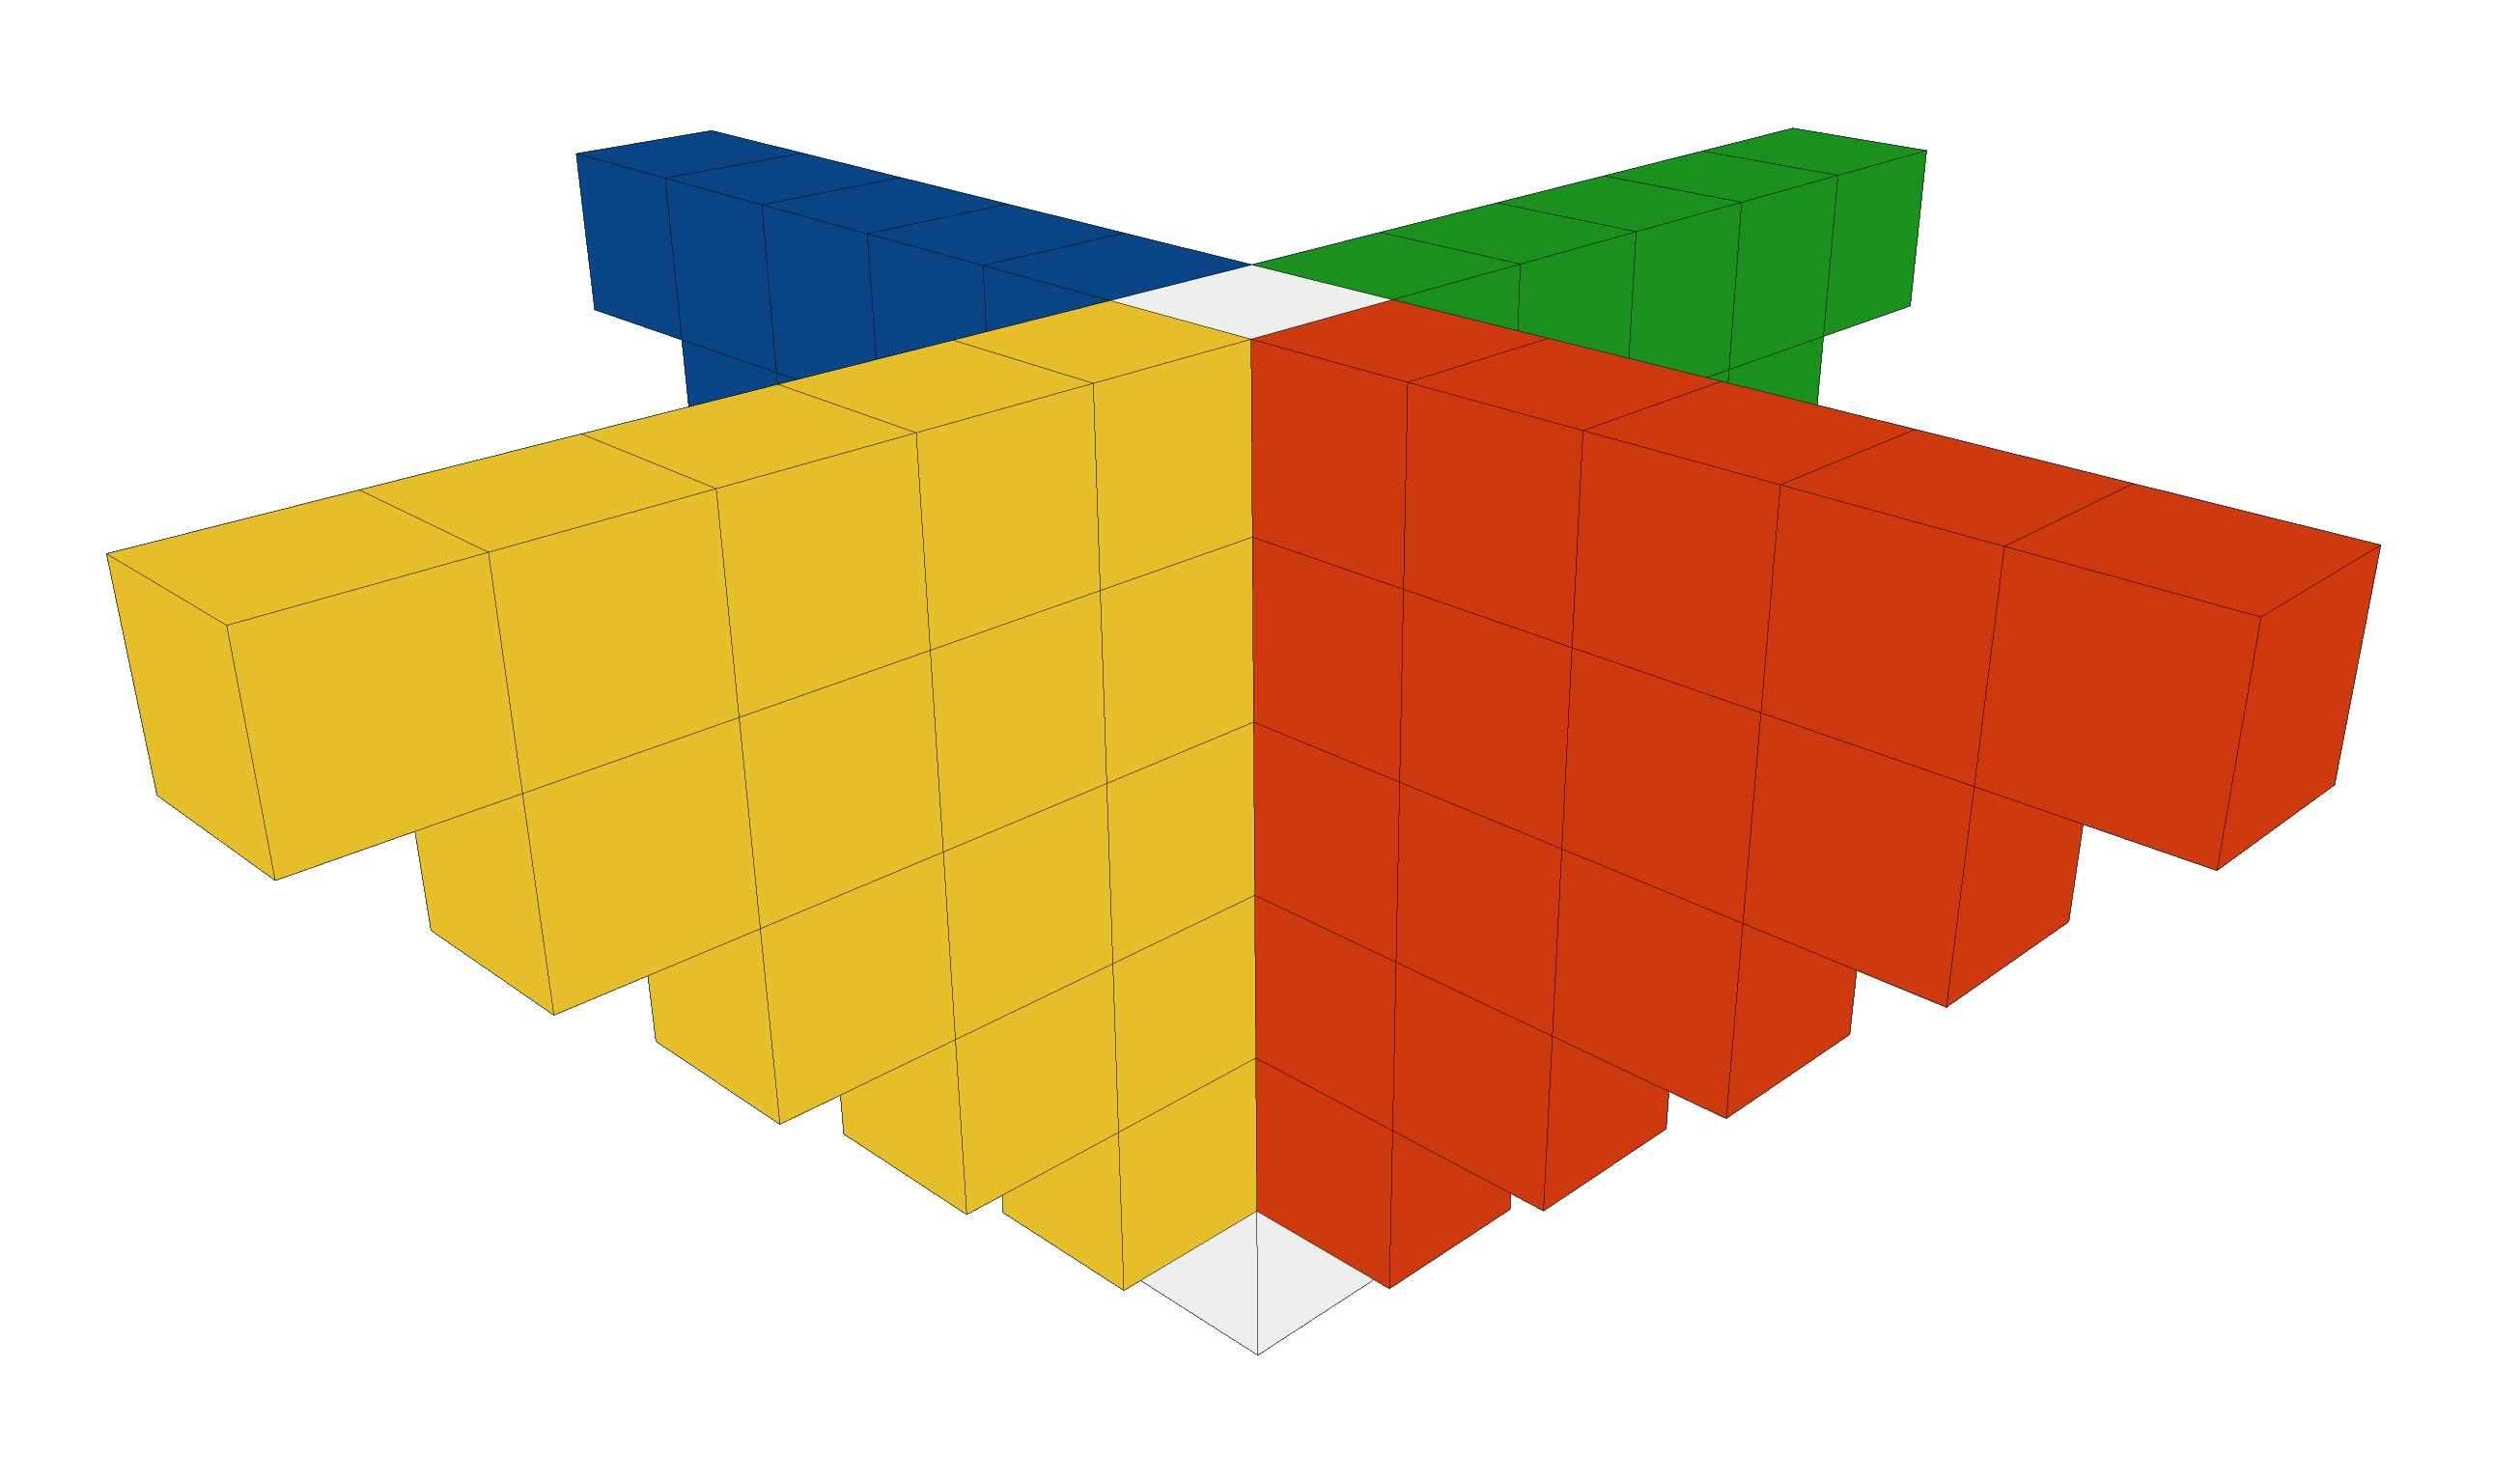
\includegraphics[height=0.1\textwidth]{../figures/angle4.png}
  \caption{Orientations of a $\bigcap_{i = 1}^4 \mathcal{L}(\mathcal{G}_i) \cap \Sigma ^6$ configuration. As $c \rightarrow \infty$, this shape approximates a tower of Hanoi whose symmetric axis joins $\sigma_i$ with orthonormal unit productions $w_i \rightarrow t_\cap$, and $[S_i \in \Lambda^*_{\sigma}]$ inhabiting the outermost bitvectors. Equations of this form are equiexpressive with linear conjunctive grammars, i.e., $\mathbb{G}^+$.}
\end{figure}

Following Okhotin~\cite{okhotin2001conjunctive}, we then extend our grammar DSL with one additional operator for combining CFGs, $\land: \mathbb{G}^+\times\mathbb{G}^+\rightarrow\mathbb{G}^+$, where $\mathbb{G}^+$ is a conjunctive grammar (CG). In our setting, CGs naturally subsume CFGs, and in so doing, observe the following denotational semantics:

\begin{prooftree}
  \hskip -0.2em
  \AxiomC{$\Gamma \vdash \mathcal{G}: \mathbb{G}$}
  \RightLabel{$+$}
  \UnaryInfC{$\Gamma \vdash \mathcal{G}: \mathbb{G}^+$}
  \DisplayProof
  \hskip 0.4em
  \AxiomC{$\Gamma \vdash \mathcal{G}, \mathcal{G}': \mathbb{G}^+$}
  \RightLabel{$\land$}
  \UnaryInfC{$\Gamma \vdash \mathcal{G} \land \mathcal{G}': \mathbb{G}^+$}
  \DisplayProof
  \hskip 0.4em
  \AxiomC{$\Gamma \vdash \sigma : \mathcal{L}(\mathcal{G})\phantom{SS}\Gamma \vdash \sigma : \mathcal{L}(\mathcal{G}')$}
  \RightLabel{$\in$}
  \UnaryInfC{$\Gamma \vdash \sigma : \mathcal{L}(\mathcal{G} \land \mathcal{G}')$}
  \DisplayProof
%  \hskip 1em
  \hskip 0.4em
  \AxiomC{$\Gamma \vdash \sigma : \mathcal{L}(\mathcal{G} \land \mathcal{G}')$}
  \RightLabel{$\cap$}
  \UnaryInfC{$\Gamma \vdash \sigma : \mathcal{L}(\mathcal{G}) \cap \mathcal{L}(\mathcal{G}')$}
  \DisplayProof
\end{prooftree}

Given two CFGs $\mathcal{G}, \mathcal{G}'$, we can compute the language intersection $\mathcal{L}(\mathcal{G})\cap\mathcal{L}(\mathcal{G}')$ by encoding $\left[(\mathcal{M}_{\mathcal{G}}^* \equiv_\sigma \mathcal{M}_{\mathcal{G}'}^*)_{i=j-1}\right]$. With this feature, we can finally express multiway intersections between two or more CFLs, which will be used to encode the bounded Levenshtein-CFL reachability problem.

%For example, we can solve $\Sigma^d \cap \overline{\mathcal{L}_\mathcal{G}}$ by enumerating $\{\beta\sigma'\gamma \mid \sigma' \in \Sigma^d, \beta = \gamma = \_^k\}$, overapproximating the prefix and suffix (padding left and right), and checking for UNSAT to underapproximate \textit{impossible substrings}, strings which cannot appear in any $\{\sigma \in \mathcal{L}_\mathcal{G}\}$. Precomputing impossible substrings for a given grammar allows us to quickly eliminate inadmissible repairs and localize syntax errors in candidate strings.

%Using the technique from \S\ref{sec:levenshtein}, we can also compute language edit distance, the minimum number of Levenshtein edits required to fix a syntactically invalid string. Language intersection is significantly faster than approximating the gradient via sampling.

%We can also build a set of grammars of increasing granularity, like a lattice structure. Basically, we can build up a lattice (in the order theoretic sense), consisting of grammars of increasing granularity. All programming languages require balanced parentheses, but some have additional constraints. So we can combine grammars, count and do bounded linear integer arithmetic.

\subsection{Levenshtein reachability}\label{sec:levenshtein}

%Levenshtein distance can be defined as an optimal transport problem between two strings $A, B: \Sigma^*$:
%
%\begin{equation}
%  \text{Levenshtein Distance} = \Delta(A, B) = \min_{\pi \in \Pi(\mu_A, \mu_B)} \int_{\Sigma^* \times \Sigma^*} \delta(A, B) d\pi(A, B)
%\end{equation}
%
%\noindent where $\mu_A$ and $\mu_B$ are the discrete distributions corresponding to strings $A$ and $B$, respectively. A single transportation plan, $\pi$, can be viewed as a sequence of Levenshtein edits, and $\Pi(\mu_A, \mu_B)$ is the set of all transport plans with marginals $\mu_A$ and $\mu_B$. Finally, the Levenshtein distance between $A$ and $B$ is then the minimum cost over all transportation plans, i.e., edit sequences $\pi \in \Pi(\mu_A, \mu_B)$.

The Levenshtein ball is finite and therefor context-free, however materializing this set is intractable for all but the smallest radii and alphabets. Instead, we dynamically instantiate a CFG that can recognize and generate the members of $\Delta_d(\err{\sigma})$ for any arbitrary $d: \mathbb{N}, \sigma: \Sigma^*$. This approach follows from a straightforward extension of Levenshtein automata~\cite{schulz2002fast}.

\begin{wrapfigure}{r}{0.5\textwidth}
  \vspace{-5pt}
  \resizebox{.5\textwidth}{!}{\begin{minipage}[c]{0.45\textwidth}
  \centering
  \underline{NIA}\vspace{10pt}
  \resizebox{\textwidth}{!}{
  \begin{tikzpicture}[
%->, % makes the edges directed
  >=stealth',
  node distance=2.5cm, % specifies the minimum distance between two nodes. Change if necessary.
%  every state/.style={thick, fill=gray!10}, % sets the properties for each ’state’ node
  initial text=$ $, % sets the text that appears on the start arrow
  ]
  \node[state, initial]                (00) {$q_{0,0}$};
  \node[state, right of=00]            (10) {$q_{1,0}$};
  \node[state, right of=10]            (20) {$q_{2,0}$};
  \node[state, right of=20]            (30) {$q_{3,0}$};
  \node[right of=30]                   (40) {$\vphantom{\vdots}\cdots$};
  \node[accepting, state, right of=40] (n0) {$q_{n,0}$};

  \node[state, above of=00]            (01) {$q_{0,1}$};
  \node[state, right of=01]            (11) {$q_{1,1}$};
  \node[state, right of=11]            (21) {$q_{2,1}$};
  \node[state, right of=21]            (31) {$q_{3,1}$};
  \node[right of=31]                   (41) {$\vphantom{\vdots}\cdots$};
  \node[accepting, state, right of=41] (n1) {$q_{n,1}$};

  \node[above of=01]                   (0j) {$\mathmakebox[\widthof{$\cdots$}]{\vdots}$};
\node[right of=0j]                   (1j) {$\mathmakebox[\widthof{$\cdots$}]{\vdots}$};
\node[right of=1j]                   (2j) {$\mathmakebox[\widthof{$\cdots$}]{\vdots}$};
\node[right of=2j]                   (3j) {$\mathmakebox[\widthof{$\cdots$}]{\vdots}$};
\node[right of=3j]                   (4j) {$\iddots$};
\node[accepting, right of=4j]        (nj) {$\mathmakebox[\widthof{$\cdots$}]{\vdots}$};

\node[state, above of=0j]            (0k) {$q_{0,k}$};
\node[state, right of=0k]            (1k) {$q_{1,k}$};
\node[state, right of=1k]            (2k) {$q_{2,k}$};
\node[state, right of=2k]            (3k) {$q_{3,k}$};
\node[right of=3k]                   (4k) {$\vphantom{\vdots}\cdots$};
\node[accepting, state, right of=4k] (nk) {$q_{n,k}$};

\draw [->] (00) edge[below] node{$\sigma_1$} (10);
\draw [->] (10) edge[below] node{$\sigma_2$} (20);
\draw [->] (20) edge[below] node{$\sigma_3$} (30);
\draw [->] (30) edge[below] node{$\sigma_4$} (40);
\draw [->] (40) edge[below] node{$\sigma_n$} (n0);

\draw [->] (01) edge[below] node{$\sigma_1$} (11);
\draw [->] (11) edge[below] node{$\sigma_2$} (21);
\draw [->] (21) edge[below] node{$\sigma_3$} (31);
\draw [->] (31) edge[below] node{$\sigma_4$} (41);
\draw [->] (41) edge[below] node{$\sigma_n$} (n1);

\draw [->] (0j) edge[below] node{$\sigma_1$} (1j);
\draw [->] (1j) edge[below] node{$\sigma_2$} (2j);
\draw [->] (2j) edge[below] node{$\sigma_3$} (3j);
\draw [->] (3j) edge[below] node{$\sigma_4$} (4j);
\draw [->] (4j) edge[below] node{$\sigma_n$} (nj);

\draw [->] (0k) edge[below] node{$\sigma_1$} (1k);
\draw [->] (1k) edge[below] node{$\sigma_2$} (2k);
\draw [->] (2k) edge[below] node{$\sigma_3$} (3k);
\draw [->] (3k) edge[below] node{$\sigma_4$} (4k);
\draw [->] (4k) edge[below] node{$\sigma_n$} (nk);

\draw [->] (00) edge[left] node{$*$}         (11);
\draw [->] (10) edge[left] node{$*$}         (21);
\draw [->] (20) edge[left] node{$*$}         (31);
\draw [->] (30) edge[left] node{$*$}         (41);
\draw [->] (30) edge[bend right, below] node{$\sigma_5$} (41);
\draw [->] (40) edge[           right] node{$\sigma_n$}  (n1);
\draw [->] (40) edge[bend right, left] node{$*$}         (n1);

\draw [->] (01) edge[left] node{$*$}                     (1j);
\draw [->] (11) edge[left] node{$*$}                     (2j);
\draw [->] (21) edge[left] node{$*$}                     (3j);
\draw [->] (31) edge[left] node{$*$}                     (4j);
\draw [->] (31) edge[bend right, below] node{$\sigma_5$} (4j);
\draw [->] (41) edge[           right] node{$\sigma_n$}  (nj);
\draw [->] (41) edge[bend right, left] node{$*$}         (nj);

\draw [->] (0j) edge[left] node{$*$}                     (1k);
\draw [->] (1j) edge[left] node{$*$}                     (2k);
\draw [->] (2j) edge[left] node{$*$}                     (3k);
\draw [->] (3j) edge[left] node{$*$}                     (4k);
\draw [->] (3j) edge[bend right, below] node{$\sigma_5$} (4k);
\draw [->] (4j) edge[           right] node{$\sigma_n$}  (nk);
\draw [->] (4j) edge[bend right, left] node{$*$}         (nk);

\draw [->] (00) edge[bend left, left] node{$*$}   (01);
\draw [->] (10) edge[bend left, left] node{$*$}   (11);
\draw [->] (20) edge[bend left, left] node{$*$}   (21);
\draw [->] (30) edge[bend left, left] node{$*$}   (31);
\draw [->] (40) edge[right] node{$*$}             (41);
\draw [->] (n0) edge[bend right, right] node{$*$} (n1);

\draw [->] (01) edge[bend left, left] node{$*$}   (0j);
\draw [->] (11) edge[bend left, left] node{$*$}   (1j);
\draw [->] (21) edge[bend left, left] node{$*$}   (2j);
\draw [->] (31) edge[bend left, left] node{$*$}   (3j);
\draw [->] (41) edge[right] node{$*$}             (4j);
\draw [->] (n1) edge[bend right, right] node{$*$} (nj);

\draw [->] (0j) edge[bend left, left] node{$*$}   (0k);
\draw [->] (1j) edge[bend left, left] node{$*$}   (1k);
\draw [->] (2j) edge[bend left, left] node{$*$}   (2k);
\draw [->] (3j) edge[bend left, left] node{$*$}   (3k);
\draw [->] (4j) edge[right] node{$*$}             (4k);
\draw [->] (nj) edge[bend right, right] node{$*$} (nk);

\draw [->] (00) edge[below] node{$\sigma_2$}    (21);
\draw [->] (10) edge[below] node{$\sigma_3$}    (31);
\draw [->] (20) edge[below] node{$\sigma_4$}    (41);

\draw [->] (01) edge[below] node{$\sigma_2$}    (2j);
\draw [->] (11) edge[below] node{$\sigma_3$}    (3j);
\draw [->] (21) edge[below] node{$\sigma_4$}    (4j);

\draw [->] (0j) edge[below] node{$\sigma_2$}    (2k);
\draw [->] (1j) edge[below] node{$\sigma_3$}    (3k);
\draw [->] (2j) edge[below] node{$\sigma_4$}    (4k);

%https://tex.stackexchange.com/a/20986/139648
\draw [decorate,decoration={brace,amplitude=10pt,raise=10pt,mirror}] (00.south west) -- (n0.south east) node[midway,yshift=-3em]{\textbf{String length}};
\draw [decorate,decoration={brace,amplitude=10pt,raise=20pt}] (00.south west) -- (0k.north west) node[midway,xshift=-40pt,rotate=90]{\textbf{Levenshtein edit distance}};
\end{tikzpicture}
}
\end{minipage}
\hfill
\begin{minipage}[l]{5 cm}
\centering
\underline{CFG}\vspace{7pt}
\begin{align*}
S &\Rightarrow \{\cdot \in Q \mid \delta(\cdot, q_{n,0}) \leq k\}\\
* &\Rightarrow \{\cdot \in \Sigma\}\\
\big\{q_{i, j} &\Rightarrow \{q_{i, j-1}*\} \mid i, j \in [1, n]\times[1, k]\big\}\\
\big\{q_{i, j} &\Rightarrow \{q_{i-1, j-1}*\}\mid i, j\in[1, n]\times [1, k]\big\}\\
\big\{q_{i, j} &\Rightarrow \{q_{i-1, j} \sigma_i \}\mid i, j \in [1, n]\times[0, k]\big\} \\
\big\{q_{i, j} &\Rightarrow \{q_{i-2, j-1} \sigma_i\} \mid i, j \in [2, n]\times[1, k] \big\}\\
\end{align*}
\end{minipage}}
  \caption{Levenshtein reachability from $\Sigma^n$ can be described as an NFA, or a left-linear CFG.}
\end{wrapfigure}

In the case where $\sigma$ and $\sigma'$ are both fixed strings, Levenshtein distance can be interpreted as a shortest path problem over an unweighted graph whose vertices are the strings $\sigma, \sigma'$, and all possible intermediate editor states, and edges represent the Levenshtein edits. Thus viewed, the Levenshtein distance between $\sigma$ and $\sigma'$ is simply the geodesic distance~\cite{ruth2023levenshtein}. When $\sigma'$ is instead a free variable and the distance is fixed, we can define a finite automaton accepting all and only strings within Levenshtein distance $d$ of $\sigma$ by unrolling the transition dynamics $\mathcal{L}(\sigma, d)$ up to a fixed horizon $d$.

Levenshtein reachability, then, is recognizable by the nondeterministic infinite automaton (NIA) whose topology $\mathcal{L} = \knightkingarrow$ factorizes into a product of (a) the monotone Chebyshev topology $\kingarrow$, equipped with horizontal transitions accepting $\sigma_{i}$ and vertical transitions accepting Kleene stars, and (b) the monotone knight's topology $\knightarrow$, equipped with transitions accepting $\sigma_{i+2}$. The structure of this space is approximated by an acyclic NFA, populated by accept states within radius $k$ of $q_{n,0}$, or equivalently, a left-linear CFG whose productions bisimulate the NFA.

\subsection{Bounded Levenshtein-CFL reachability}\label{sec:editreach}

%Assume a hypothetical $\Phi(\mathcal{G}': \mathbb{G}, \err{\sigma}: \Sigma^*)\mapsto \tilde{\sigma}: \mathcal{L}(\mathcal{G}')$ which takes a CFG, $\mathcal{G}'$, generating an arbitrary nonempty CFL, and an unparseable string, $\err{\sigma}$, and which returns element(s) of $\mathcal{L}(\mathcal{G}')$ most similar to $\err{\sigma}$ according to their Levenshtein distance $\Delta(\err{\sigma}, \cdot)$.

\begin{wrapfigure}{r}{0.33\textwidth}
  \vspace{-10pt}
  \resizebox{0.33\textwidth}{!}{\begin{tikzpicture}[
  dot/.style = {circle, inner sep=0pt, minimum size=1mm, fill,
  node contents={}}
]
  \def\firstcircle{(-2.1,0) coordinate (a) circle (2.4cm)}
  \def\firstcirclea{(-2.1,0) coordinate (b) circle (0.6cm)}
  \def\firstcircleb{(-2.1,0) coordinate (c) circle (1.2cm)}
  \def\firstcirclec{(-2.1,0) coordinate (d) circle (1.8cm)}
  \def\secondcircle{(1.2,0) coordinate (e) circle (1.5cm)}
  \begin{scope}
    \clip \secondcircle;
    \fill[black!15] \firstcircle;
  \end{scope}
  \draw \firstcircle node[dot,label=$\err{\sigma}$](z0);
  \draw [dashed] \firstcirclea;
  \draw [dashed] \firstcircleb;
  \draw [dashed] \firstcirclec;
  \draw[-stealth] (-2.1,0) -- (-1.5, 0) node[midway,below]{$d_1$};
  \draw[-stealth] (-1.5,0) -- (-0.9, 0) node[midway,below]{$d_2$};
  \draw[-stealth] (-0.9,0) -- (-0.3, 0) node[midway,below]{$\vphantom{d}\ldots$};
  \draw[-stealth] (-0.3,0) -- (0.3, 0) node[midway,below]{$d^*$};
  \draw[-stealth] (-0.3,0) -- (0.3, 0) node[midway,above]{$\tilde{\sigma}$};
  \draw \secondcircle;
  \node [above] at (current bounding box.north -| a) {$\mathcal{L}(G(\err\sigma, d^*))$};
  \node [above,yshift=1.5cm] at (e) {$\mathcal{L}(\mathcal{G}')$};
\end{tikzpicture}}
  \caption{LED is computed gradually by incrementing $d$ until $\mathcal{L}^\cap_{d}\neq \varnothing$.}
\end{wrapfigure}

Let $G(\err{\sigma}: \Sigma^*, d: \mathbb{N}^+) \mapsto \mathbb{G}$ be the specific construction described in \S\ref{sec:levenshtein} which accepts a string, $\err{\sigma}$, and an edit distance, $d$, and returns a grammar representing the NFA that recognizes the language of all strings within Levenshtein radius $d$ of $\err{\sigma}$. To find the language edit distance and corresponding least-distance edits, we must find the smallest $d$ such that $\mathcal{L}^\cap_d$ is nonempty, where $\mathcal{L}^\cap_d$ is defined as $\mathcal{L}\bigl(G(\err\sigma, d)\bigr) \cap \mathcal{L}(\mathcal{G}')$. In other words, we seek $\tilde{\sigma}$ and $d^*$ under which three criteria are all satisfied:\linebreak (1) $\tilde{\sigma}\in\mathcal{L}(\mathcal{G}')$, and (2) $\Delta(\err{\sigma}, \tilde{\sigma}) \leq d^* \Longleftrightarrow \tilde{\sigma} \in \mathcal{L}\bigl(G(\err{\sigma}, d^*)\bigr)$, and (3) $\not\exists \sigma' \in \mathcal{L}(\mathcal{G}').\bigl[\Delta(\err{\sigma}, \sigma') < d^*\bigr]$. To satisfy these criteria, it suffices to check $d \in (1, d^*]$ by encoding the Levenshtein automata and the original grammar as a single SAT formula, call it, $\varphi_d(\cdot)$, and gradually admitting new acceptance states at increasing radii. If $\varphi_d(\cdot)$ returns UNSAT, $d$ is increased until either (1) a satisfying assignment is found or (2) $d^*$ is attained. Following~\ref{lemma:upper-bound}, this procedure is guaranteed to terminate in at most either (1) the number of steps required to overwrite every symbol in $\err{\sigma}$, or (2) the length of the shortest string in $\mathcal{L}(\mathcal{G}')$, whichever is greater. When $\mathcal{L}(\mathcal{G}')$ is context-free, $\mathcal{L}^\cap_d$ provably context-free using the Bar-Hillel construction~\cite{bar1961formal}, however in general, the resulting intersection is a conjunctive language.
%More precisely, we can define $\varphi_d(\cdot)$ as follows:
%
%\begin{equation}
%\varphi_{d+1}(\mathcal{G}', \err{\sigma}) \coloneqq \begin{cases}
%\varphi\bigl[\tilde{\sigma}\in\mathcal{L}\bigl(G(\err\sigma, d)\bigr) \land \tilde{\sigma}\in \mathcal{L}(\mathcal{G}')\bigr] & \text{if $d=1$ or $\varphi_d(\cdot)$ is SAT}.\\
%\varphi_{d} \oplus \bigoplus_{\{q \in Q \mid \delta(q, q_{n,0}) = d+1\}}\varphi[S \rightarrow q] & \text{if $d \leq \max(|\err{\sigma}|, \min_{\sigma \in \mathcal{L}(\mathcal{G}')}|\sigma|)$}.
%\end{cases}
%\end{equation}

%\noindent The function $\varphi_{d+1}(\mathcal{G}', \err{\sigma})$ is a realizer of $\Phi$.

%Alternatively, we can overapproximate $d^*$ using $d^+$, sample the overapproximated region and minimize the resulting patches using the minimization approach described in

%By intersection with a CFG, $\mathcal{G}'$, Bar-Hillel ensures the resulting language will remain context-free.
%
%We then intersect that language with $\Sigma^n$ and $\mathcal{L}(\mathcal{G})$, the original grammar, to obtain a finite set.

\subsection{Tensor sparsification}\label{sec:sparsity}

Although we can encode $[\mathcal{M}_\sigma = \mathcal{M}^2_\sigma]$ explicitly, na\"ively encoding the formula as a dense constraint system is highly suboptimal. For starters, we can always ignore all lower-triangular comparisons $\{\mathcal{M}_{ij} \mid i \geq j\}$. A considerably sparser but logically equivalent representation that avoids many elementwise comparisons in the upper-triangular region can be achieved by analyzing the specific string and grammar in question. Since we are typically interested in strings with at least some bound variables, $\{\sigma: \underline\Sigma^n \mid \exists \sigma_i \in \Sigma\}$, there is likely to be many upper-triangular nonterminals $\langle v, i, j\rangle \subset V\times\{i, j \mid 0 \leq i \leq j \leq |\sigma|)\}$ that are incompatible with $\sigma$, i.e., which are unreachable from $\sigma_{i\ldots j}$ regardless of which values they assume. We call these elements \textit{impossible nonterminals}.

\begin{definition}[Impossible nonterminals]
  Given $\sigma: \underline\Sigma^n$ and $\mathcal{G}: \mathbb{G}$, an impossible nonterminal is a triple $\langle v, i, j\rangle: V\times\{i, j \mid 0 \leq i \leq j \leq |\sigma|)\}$ such that $\forall \sigma': \Sigma^{j-i}, \sigma' \in \text{H}(\sigma_{i\ldots j}) \implies v\notin\Lambda^*_{\sigma'}$.
\end{definition}

We can immediately rule out nonterminals absent from the parse forest of any static substring.

\begin{lemma}
  Given $\sigma, \langle v, i, j \rangle$, if $\sigma_{i\ldots j}: \highlight{\Sigma^*}$ and $v \not\in \Lambda^*_{\sigma_{i \ldots j}}$ hold, this implies $\langle v, i, j \rangle$ is impossible.
\end{lemma}

We will now show how it is possible to discharge many nonterminal triples by considering the CFG reachability of $v$ in relation to its position $\mathcal{M}_{i, j}$ and $n$, irrespective of the specific string $\sigma$.

\begin{definition}[CFG reachability]
%  Let $\Rightarrow^*_\mathcal{G}$ be the reflexive transitive closure under $\mathcal{G}$ defined in the usual way.
  Let us define a reachability relation $R(\nu, \mu, \eta)$ over CFGs as $\{\langle\nu, \mu, \eta\rangle: (\Sigma \cup V)^2\times\mathbb{N} \mid \exists\:\alpha, \beta: (V\cup\Sigma)^*, \nu \Rightarrow^{\leq \eta}_\mathcal{G} \alpha \mu \beta\}$. We write $T^\eta(U)$ to denote the set of all $t: \Sigma \cup V$ where there exists $u\in U$ such that $R(u, t, \eta)$, and likewise $T^{-\eta}(U)$ to denote ``\ldots'' $R(t, u, \eta)$.
  %$R(\mu, \nu, n)$ and $R(\nu, \mu, n)$ respectively
\end{definition}

\begin{lemma}
  Given $n, \langle v, i, j \rangle$, if $v \notin T^{i-j}(\Sigma)$, this implies $v\not\Rightarrow^{\leq j-i}_\mathcal{G} \Sigma^{j-i}$ and therefor $\langle v, i, j \rangle$ must be impossible. Furthermore, if $v \notin T^{n-j+i}(\{S\})$, then $S\not\Rightarrow^{\leq n-j+i}_\mathcal{G} v$ and therefor $\langle v, i, j \rangle$ must be impossible.
\end{lemma}

Regardless of $\sigma$, it is always possible to discharge nonterminals inhabiting $\Lambda_{i, j}$ bitvectors outside the $(n-j+i)$-step neighborhood of $S$, or the $(j-i)$-step neighborhood of any terminal due to unreachability. This constrains several of the least- and greatest- upper diagonals of $\mathcal{M}_\sigma$. Further improvements to sparsity can be achieved by considering the specific structure of $\sigma$ and $\mathcal{G}$.

\begin{definition}[Parikh image]
  Let $\pi: \underline\Sigma^*\rightarrow\mathbb{N}^{|\Sigma|}$ be the Parikh vector~\cite{parikh1966context}, which counts the number of times each terminal appears in a string. We define the Parikh image as the set of all terminals indexed a nonzero element of the Parikh vector, i.e., $\Pi(\sigma:\underline\Sigma^*) \coloneq \{\sigma': \Sigma \mid 0 < \pi(\sigma)[\sigma']\}$. %Ordered by inclusion, the set of all minimal Parikh images, $\Pi^*(\sigma)\coloneqq \min_{\bm\sigma : 2^V \mid \forall \sigma' \in \bm\sigma \sigma' \in \text{H}(\sigma) \text{ and } }$ forms a partial order.
\end{definition}

\begin{lemma}
Given $\sigma, \langle v, i, j \rangle$, then $\Pi(\sigma_{i\ldots j}) \not\subseteq T^\infty(\{v\})$ implies $v\not\Rightarrow^*_\mathcal{G} \sigma_{i\ldots j}$ and $\langle v, i, j \rangle$ is impossible.
\end{lemma}

We can overapproximate the set of possible nonterminals by comparing the Parikh image of $\sigma_{i\ldots j}$ with the closure of $v$, then discharging impossible nonterminal triples $\langle v, i, j \rangle$. If $\Pi(\sigma_{i\ldots j}) \not\subseteq T^\infty(\{v\})$, then we know $\sigma_{i\ldots j}$ cannot derive $v$ and $\left[(\mathcal{M}_{\sigma} = \mathcal{M}_{\sigma}^2)_{i, j, v}\right]$ may be safely ignored. Note that a tighter approximation can be achieved by considering the minimal Parikh vectors of all $\sigma: \Sigma^\eta$ such that $v \Rightarrow_\mathcal{G}^* \sigma \in \text{H}(\sigma_{i\ldots j})$, rather than just the image on $V$, however this would be computationally more expensive and $\Pi(\sigma)$ already discharges a large fraction of impossible nonterminals in practice.

\subsection{Isolation and reduction}

\newcommand\ddd{\Ddots}
\newcommand\vdd{\Vdots}
\newcommand\cdd{\Cdots}
\newcommand\lds{\ldots}
\newcommand\vno{\varnothing}
\newcommand{\ts}[1]{\textsuperscript{#1}}
\newcommand\non{1\ts{st}}
\newcommand\ntw{2\ts{nd}}
\newcommand\nth{3\ts{rd}}
\newcommand\nfo{4\ts{th}}
\newcommand\nfi{5\ts{th}}
\newcommand\nsi{6\ts{th}}
\newcommand\nse{7\ts{th}}
\newcommand{\vs}[1]{\sigma_{#1}^{\shur}}
\newcommand{\gs}[1]{\gamma_{#1}^{\shur}}
\newcommand{\bs}[1]{\beta_{#1}^{\shur}}
\newcommand{\qs}[1]{\alpha_{#1}^{\shur}}
\newcommand\rcr{\rowcolor{black!15}}
\newcommand\rcw{\rowcolor{white}}
\newcommand\pcd{\cdot}
\newcommand\pcp{\phantom\cdot}
\newcommand\ppp{\phantom{\nse}}
\newcommand\hhg[1]{\tikz[overlay]\node[rectangle,fill=black!15,draw=none,text opacity =1] {$#1$};}

\begin{wrapfigure}{r}{0.4\textwidth}
  \vspace{-20pt}
  \resizebox{0.4\textwidth}{!}{\[
  \mathbf{M}^* = \begin{pNiceArray}{ccccccc}[margin, extra-margin=2pt,colortbl-like, xdots/line-style=loosely dotted]
                   \vno & \rcr \vs{1} & \mathcal{L}_{1,3} & \mathcal{L}_{1,3} & \rcw \mathcal{V}_{1,4} & \cdd & \mathcal{V}_{1,n} \\
                   \vdd & \ddd        & \rcr\vs{2}        & \mathcal{L}_{2,3} & \rcw\vdd               &      & \vdd \\
                   &             &                   & \rcr\vs{3}        & \rcw                   &      & \\
                   &             &                   &                   & \mathcal{V}_{4,4}      &      & \\
                   &             &                   &                   &                        & \ddd & \\
                   &             &                   &                   &                        &      & \mathcal{V}_{n,n} \\
                   \vno & \cdd        &                   &                   &                        &      & \vno
  \end{pNiceArray} \equiv
  \begin{pNiceArray}{ccccc}[margin, extra-margin=2pt,colortbl-like, xdots/line-style=loosely dotted]
    \vno & \rcr\mathcal{L}_{1,3} & \rcw\mathcal{V}_{1,4} & \cdd & \mathcal{V}_{1,n} \\
    \vdd & \ddd                  & \mathcal{V}_{2,4}     &      & \vdd \\
    &                       &                       & \ddd & \\
    &                       &                       &      & \mathcal{V}_{n,n} \\
    \vno & \cdd                  &                       &      & \vno
  \end{pNiceArray}
\]}
  \caption{When is this reduction admissible?}\label{fig:mat_simpl}
  \begin{center}\resizebox{0.35\textwidth}{!}{\begin{center}
\begin{equation*}
  M^*(\mathcal{G}, \beta\alpha\gamma)=
\begin{tikzpicture}[
  scale=0.4,
  baseline,
  label distance=10pt % added
]

\matrix [matrix of math nodes,left delimiter=(,right delimiter=),row sep=0.1cm,column sep=0.1cm] (m) {
\varnothing & \beta_1^\shri & \phantom{\cdots} & \,\Lambda_{\beta}\,  &        &                      & \phantom{\qs{|\alpha|}} &        &                      & \smash{\Lambda_{\beta\alpha\gamma}^*}      \\
            &               & \phantom{\ddots} & \phantom{\vdots}     &        & \bm\Lambda_\alpha^\shup &                  &        &                      &        \\
            &               &                  & \bs{|\beta|}         &        &                      &                  &        &                      & \phantom{\bs{|\beta|}}       \\
            &               &                  &                      & \qs{1} & \phantom{\cdots}     & \Lambda_{\alpha} &        &                      & \phantom{\vs{j}} \\
            &               &                  &                      &        & \phantom{\ddots}     & \phantom{\vdots} &        & \bm\Lambda_\alpha^\shri &        \\
            &               &                  &                      &        &                      & \qs{|\alpha|}           &        &                      & \phantom{\qs{|\alpha|}}      \\
            &               &                  &                      &        &                      &                  & \gs{1} & \phantom{\cdots}     & \Lambda_{\gamma}\vphantom{\gs{1}} \\
            &               &                  &                      &        &                      &                  &        & \phantom{\ddots}     & \phantom{\vdots} \\
            &               &                  &                      &        &                      &                  &        &                      & \gamma_{|\gamma|}^\shup      \\
\varnothing &               &                  &                      &        &                      &                  &        &                      & \varnothing\\
};

\draw[loosely dotted] (m-1-1.south) -- (m-10-1.north);
\draw[loosely dotted] (m-1-1.south east) -- (m-10-10.north west);
\draw[loosely dotted] (m-10-1.east) -- (m-10-10.west);

% β
\draw[loosely dotted] (m-1-2.south east) -- ([xshift=0.3cm]m-3-4.north west);
\draw[loosely dotted] (m-1-2.east) -- (m-1-4.west);
\draw[loosely dotted] (m-1-4.south) -- (m-3-4.north);

\draw[dashed] (m-1-4.north east) -- (m-3-4.south east);
\draw[dashed] (m-3-4.south east) -- (m-3-10.south east);
\draw[dashed] (m-1-7.north east) -- (m-6-7.south east);
\draw[dashed] (m-6-7.south east) -- (m-6-10.south east);

% α
\draw[loosely dotted] (m-4-5.south east) -- ([xshift=0.45cm,yshift=-0.2cm]m-6-7.north west);
\draw[loosely dotted] (m-4-5.east) -- (m-4-7.west);
\draw[loosely dotted] (m-4-7.south) -- (m-6-7.north);

% γ
\draw[loosely dotted] (m-7-8.south east) -- ([xshift=-0.1cm,yshift=-0.3cm]m-9-10.north west);
\draw[loosely dotted] (m-7-8.east) -- (m-7-10.west);
\draw[loosely dotted] (m-7-10.south) -- (m-9-10.north);
\node[
    fit=(m-1-2)(m-1-4),
    inner xsep=0,inner ysep=10pt,
    above delimiter=\{,
    label=above:$\beta$
] {};

\node[
    fit=(m-7-10)(m-9-10),
    inner xsep=14pt,inner ysep=0,
    right delimiter=\},
    label=right:$\gamma$
] {};

\end{tikzpicture}
\end{equation*}
\end{center}}\end{center}
  \caption{We can inspect $\bm\Lambda_\alpha^\shri, \bm\Lambda_\alpha^\shup$ to find out.}
\end{wrapfigure}

Depicted right is a SAT tensor representing \hlgray{$\sigma_1\:\sigma_2\:\sigma_3$}$\:\_\:\ldots\:\_$ where shaded regions demarcate known bitvector literals $\highlight{\Lambda_{r,c}}$ (i.e., representing established nonterminal forests) and unshaded regions correspond to bitvector variables $\Lambda_{r,c}$ (i.e., representing unknown nonterminal forests to be solved) for an incomplete string. Since $\highlight{\Lambda_{r,c}}$ are fixed, we can precompute them outside of the SAT solver.

Clearly, formula complexity is heavily dependent on $|\sigma|$ and for the sake of complexity, it would be highly advantageous if $\sigma$ were shorter. Naturally, this raises the question of when well-formed substrings can be collapsed, i.e., under what circumstances can the reduction in Fig.~\ref{fig:mat_simpl} be applied? This transformation is admissible when a subexpression is ``isolated'', i.e., its derivation cannot somehow be altered by appending or prepending text. For example, the string \texttt{( - b )} is \textit{isolated} in the sense that adjoining text should not alter the interior derivation, whilst \texttt{- b} is not, as adjacent text (e.g., \texttt{\hlgreen{a} - b}) may alter the derivation of its contents. This question can be reduced to a quotient: does there exist any string, that when so adjoined will ``strip away'' any nonterminals, leading to another derivation?

More formally, given an arbitrary (potentially ambiguous) context free grammar $\mathcal{G}: \mathbb{G}$, and string $\alpha: \Sigma^*$, is there a decision procedure that returns whether appending and/or prepending symbols can alter the parse forest of $\alpha$? In other words, we want a function $F: (\mathbb{G} \times \Sigma^*) \rightarrow \mathbb{B}$ that returns whether $\alpha$'s parse forest according to $\mathcal{G}$ is unique over $\beta\alpha\gamma$, for all $\beta, \gamma: \underline\Sigma^*$. Specifically,

\begin{definition}[Isolation]\label{def:isolation}
Let $T_\alpha$ denote the set of all parse trees that are generated by the string $\alpha$ using $\mathcal{G}$, and consider $\mathbf{T}_{\alpha}$, the union of all parse trees and their subtrees that can be generated by $\beta\alpha\gamma$ using $\mathcal{G}$ for arbitrary $\beta, \gamma \in \underline\Sigma^*$, and have a leaf in $\alpha$. We call the parse forest $T_\alpha$ \textit{isolated} iff for all $t \in \mathbf{T}_{\alpha}$, there exists $t' \in T_\alpha$, such that $t$ is either a subtree of $t'$, or $t'$ is a proper subtree of $t$.
\end{definition}

If we can identify an $\alpha: \Sigma^*$ where $\alpha = \sigma_{i\ldots j}$ for some $i, j: \mathbb{N}^{<|\sigma|}$, such that $\alpha$ has an isolated parse forest, then we can safely replace $\sigma_{i\ldots j} \mapsto \Lambda_\alpha^*$. For bounded-length strings, this can be solved by padding $\alpha$ with adjacent holes $(\_)^n\alpha(\_)^n$ for sufficiently large $n$, and checking $\bm\Lambda_{\alpha}^{\shur}$, the union of all right- and left-quotients of $\alpha$ for emptiness, i.e., $[\varnothing = \bm\Lambda_{\alpha}^\shup\cup\bm\Lambda_{\alpha}^\shri]$. A general solution for arbitrary CFGs, $\mathcal{G}: \mathbb{G}$ and $\beta, \gamma \in \Sigma^*$ is more difficult, but could significantly extend the context window and remove the need for ad hoc preprocessing. We leave this as an open problem for future work.
%
%Claim #1: The parse forest for $\alpha$ is unique when $\bm\Lambda_{\alpha}^{\shur} = \varnothing$.
%
%Question: Claim #1 is sufficient, but is it necessary?

\subsection{Sampling the Levenshtein ball without replacement in $\mathcal{O}(1)$}\label{sec:dsi}

Now that we have a reliable method to synthesize admissible completions for strings containing holes, i.e., fix \textit{localized} errors, $F: (\mathcal{G} \times \underline\Sigma^n) \rightarrow \{\Sigma^n\}\subseteq \mathcal{L}(\mathcal{G})$, how can we use $F$ to repair some unparseable string, i.e., $\err{\sigma_1\ldots\:\sigma_n}: \Sigma^n \cap\mathcal{L}(\mathcal{G})^\complement$ where the holes' locations are unknown? Three questions stand out in particular: how many holes are needed to repair the string, where should we put those holes, and how ought we fill them to obtain a parseable $\tilde{\sigma} \in \mathcal{L}(\mathcal{G})$?

One plausible approach would be to draw samples with a PCFG, minimizing tree-edit distance, however these are computationally expensive metrics and approximations may converge poorly. A more efficient strategy is to sample string perturbations, $\bm{\sigma}\sim\Sigma^{n\pm q}\cap\Delta_{q}(\err{\sigma})$ uniformly across the Levenshtein q-ball centered on $\err{\sigma}$, i.e., the space of all admissible edits with Levenshtein distance $\leq q$, loosely analogous to a finite difference approximation over words in a finite language.

To implement this strategy, we first construct a surjection $\varphi^{-1}: \mathbb{Z}_2^m\twoheadrightarrow\Delta_{q}(\err{\sigma})$ from bitvectors to Levenshtein edits over $\err\sigma, \Sigma$, sample bitvectors without replacement using a characteristic polynomial, then decode the resulting bitvectors into Levenshtein edits. This ensures the sampler eventually visits every Levenshtein edit at least exactly once and at most approximately once, without needing to store any samples in memory, and discovers a steady stream of admissible edits throughout the solving process, independent of the grammar or string under repair.

More specifically, we employ a pair of [un]tupling functions $\kappa, \rho: \mathbb{N}^k \leftrightarrow \mathbb{N}$ which are (1) bijective (2) maximally compact (3) computationally tractable (i.e., closed form inverses). $\kappa$ will be used to index $\stirlingii{n}{k}$\footnote[2]{\text{Following Stirling, we use the notation $\stirlingii{n}{d}$ to denote the set of all $d$-element subsets of $\{1,\ldots, n\}$.}}-combinations via the Maculay representation~\cite{knuth2005taocp} and $\rho$ will index $\Sigma^k$ tuples, but is slightly more tricky to define. To maximize compactness, there is an elegant pairing function courtesy of Szudzik~\cite{szudzik2006elegant}, which enumerates concentric square shells over the plane $\mathbb{N}^2$ and can be generalized to hypercubic shells in $\mathbb{N}^k$. For our purposes, this generalization will suffice.

Although $\langle\kappa, \rho\rangle$ could be used directly to exhaustively search the Levenshtein ball, they are temporally biased samplers due to lexicographic ordering. Rather, we would prefer a path that uniformly visits every fertile subspace of the Levenshtein ball over time regardless of the grammar or string in question: subsequences of $\langle\kappa, \rho\rangle$ should discover valid repairs with frequency roughly proportional to the filtration rate, i.e., the density of the admissible set relative to the Levenshtein ball. These additional constraints give rise to two more criteria: (4) ergodicity and (5) periodicity.

\begin{wrapfigure}{r}{0.35\textwidth}
  \vspace{-10pt}
  \begin{minipage}{.35\textwidth}
    \begin{align*}
      U^\intercal Y = \begin{pNiceMatrix}[nullify-dots,xdots/line-style=loosely dotted]
                        C_1    & \cdd  &       &       & C_m \\
                        \top   & \circ & \cdd  &       & \circ \\
                        \circ  & \ddd  & \ddd  &       & \vdd \\
                        \vdd   & \ddd  &       &       & \\
                        \circ  & \cdd  & \circ & \top  & \circ
      \end{pNiceMatrix}^t
      \begin{pNiceMatrix}[nullify-dots,xdots/line-style=loosely dotted]
        Y_1 \\
        \vdd\\
        \\
        \\
        Y_m
      \end{pNiceMatrix}\label{eq:lfsr}
    \end{align*}
  \end{minipage}
\end{wrapfigure}

To achieve ergodicity, we permute the elements of $\stirlingii{n}{k}\times\Sigma^k$ using a finite field with a characteristic polynomial $C$ of degree $m\coloneqq\lceil \log_b {n \choose k}|\Sigma_\varepsilon|^k \rceil$. By choosing $C$ to be some irreducible polynomial, one ensures the path has the mixing properties we desire, e.g., suppose $U: \mathbb{Z}_2^{m\times m}$ is a matrix whose structure is depicted to the right, wherein $C$ represents a primitive polynomial over $\mathbb{Z}_2^m$ with known coefficients $C_{1\ldots m}$ and semiring operators $\oplus \coloneqq + \pmod 2, \otimes \coloneqq \land, \top \coloneqq 1, \circ\coloneqq0$. Since $C$ is primitive, the sequence $\mathbf{R} = (U^{0 \ldots 2^m-1}Y)$ must have \textit{full periodicity}, i.e., for all $i, j \in[0, 2^m)$, ${\mathbf{R}_i = \mathbf{R}_j \Rightarrow i = j}$. To uniformly sample $\bm\sigma$ without replacement, we construct a partial surjective function from $\mathbb{Z}_2^m$ onto the Levenshtein ball, $\mathbb{Z}_2^m\rightharpoonup\stirlingii{n}{d}\times\Sigma_\varepsilon^{d}$, cycle over $\mathbf{R}$, then discard samples which have no witness in $\stirlingii{n}{d}\times\Sigma_\varepsilon^{d}$.

This procedure requires $\mathcal{O}(1)$ per sample and roughly ${n \choose d}|\Sigma_\varepsilon|^{d}$ samples to exhaustively search $\stirlingii{n}{d}\times\Sigma_\varepsilon^{d}$. Its acceptance rate $b^{-m}{n \choose d}|\Sigma_\varepsilon|^{d}$ can be slightly improved with a more suitable base $b$, however this introduces some additional complexity and so we elected to defer this optimization.

In addition to its statistically desirable properties, our sampler has the practical benefit of being trivially parallelizable using leapfrogging, i.e., given $p$ independent processors, each one $p_j$ can independently check $[\varphi^{-1}(\langle\kappa, \rho\rangle^{-1}(\mathbf{R}_{i}), \err{\sigma}) \in \mathcal{L}(\mathcal{G})]$ where $p_j \equiv i \pmod{|p|}$. This procedure linearly scales with the total processors, exhaustively searching $\Delta_{q}(\err{\sigma})$ in $|p|^{-1}$ of the time required by a single processor, or alternately drawing $|p|$ times as many samples in the same amount of time.

To admit variable-length edits and enable deletion, we first define a $\varepsilon^+$-production and introduce it to the right- and left-hand side of each terminal in a unit production in our grammar, $\mathcal{G}$:\vspace{5pt}

\begin{prooftree}
  \AxiomC{$\mathcal{G} \vdash \varepsilon \in \Sigma$}
  \RightLabel{$\varepsilon\textsc{-dup}$}
  \UnaryInfC{$\mathcal{G} \vdash (\varepsilon^+ \rightarrow \varepsilon \mid \varepsilon\:\varepsilon^+) \in P$}
  \DisplayProof
  \hskip 1.5em
  \AxiomC{$\mathcal{G} \vdash (A \rightarrow B) \in P$}
  \RightLabel{$\varepsilon^+\textsc{-int}$}
  \UnaryInfC{$\mathcal{G} \vdash (A \rightarrow B\:\varepsilon^+ \mid \varepsilon^+\:B \mid B) \in P$}
\end{prooftree}

Finally, to sample $\sigma\sim\Delta_{q}(\err{\sigma})$, we first interleave $\err\sigma$ as $\err\sigma_\varepsilon$ (see Lemma~\ref{lemma:interleaving}), then enumerate hole templates $\text{H}(\err\sigma_\varepsilon, i) = \sigma_{1\ldots i-1}\:\text{\_ \_}\:\sigma_{i+1\ldots n}$ for each $i \in \cdot \in \stirlingii{n}{d}$ and $d \in 1\ldots q$, then solve for $\tilde{\sigma} \in \text{H}(\err\sigma_\varepsilon, i)$ satisfying $[S \in \Lambda^*_{\tilde\sigma, \mathcal{G}}] \Leftrightarrow [\tilde\sigma \in \mathcal{L}(\mathcal{G})]$. If $\bm\sigma \coloneqq \text{H}(\err\sigma_\varepsilon, i)$ is nonempty, then each edit from each patch in each $\tilde{\sigma} \in \bm\sigma$ will match one of the following patterns, covering all three Levenshtein edits:\vspace{-10pt}

\begin{align*}
    \text{Deletion}&=\begin{cases}
                         \,\ldots\sigma_{i-1}\:\text{\hlred{$\gamma_1$}\:\hlred{$\gamma_2$}}\:\sigma_{i+1}\ldots\hspace{0.2cm}\gamma_{1, 2} = \varepsilon\label{eq:del}
    \end{cases}\\
    \text{Substitution}&=\begin{cases}
                             \ldots\sigma_{i-1}\:\text{\hlorange{$\gamma_1$}\:\hlred{$\gamma_2$}}\:\sigma_{i+1}\ldots\hspace{0.2cm}\gamma_1 \neq \varepsilon \land \gamma_2 = \varepsilon\\
                             \ldots\sigma_{i-1}\:\text{\hlred{$\gamma_1$}\:\hlorange{$\gamma_2$}}\:\sigma_{i+1}\ldots\hspace{0.2cm}\gamma_1 = \varepsilon \land \gamma_2 \neq \varepsilon\\
                             \ldots\sigma_{i-1}\:\text{\hlorange{$\gamma_1$}\:\hlorange{$\gamma_2$}}\:\sigma_{i+1}\ldots\hspace{0.2cm}\{\gamma_1, \gamma_2\}\cap\{\varepsilon, \sigma_i\} = \varnothing
    \end{cases}\\
    \text{Insertion}&=\begin{cases}
                          \ldots\sigma_{i-1}\:\text{\hlgreen{$\gamma_1$}\:\hlorange{$\gamma_2$}}\:\sigma_{i+1}\ldots\hspace{0.2cm}\gamma_1 = \sigma_i \land \gamma_2 \notin \{\varepsilon,  \sigma_i\}\label{eq:ins2}\\
                          \ldots\sigma_{i-1}\:\text{\hlorange{$\gamma_1$}\:\hlgreen{$\gamma_2$}}\:\sigma_{i+1}\ldots\hspace{0.2cm}\gamma_1 \notin \{\varepsilon, \sigma_i\} \land \gamma_2 = \sigma_i\label{eq:ins1}\\
                          \ldots\sigma_{i-1}\:\text{\hlgreen{$\gamma_1$}\:\hlgreen{$\gamma_2$}}\:\sigma_{i+1}\ldots\hspace{0.2cm}\gamma_{1,2} = \sigma_i\label{eq:copy}
    \end{cases}
\end{align*}

\noindent Although complete with respect to $\Delta_{q}(\err{\sigma})$, this approach can produce patches containing more Levenshtein edits than are strictly necessary to repair $\err\sigma$. To ensure patches are both minimal and syntactically valid, we first introduce a simple technique to minimize the repairs in \S\ref{sec:minimization}. By itself, uniformly sampling minimal repairs $\tilde\sigma\sim\Delta_{q}(\err{\sigma})\cap\mathcal{L}(\mathcal{G})$ is sufficient but can be quite time-consuming, as we empirically show in \S\ref{sec:uniform}. To further reduce sample complexity and enable real-time repairs, we will then introduce a more efficient density estimator based on adaptive resampling (\S\ref{sec:adaptive}).

\subsection{Patch minimization}\label{sec:minimization}

\begin{wrapfigure}{r}{0.4\textwidth}
  \vspace{-14pt}
  \resizebox{.4\textwidth}{!}{
    $$
    \def\arl{\ar@{-}}
    \xymatrix{
      & \texttt{\hlgreen{(} a \hlorange{+} b \hlgreen{)}}\arl[dl]\arl[d]\arl[dr] & \\
      \texttt{\vphantom{)}\err{\hlgreen{(} a \hlorange{+} b}}\arl[d]\arl[dr] & \texttt{\vphantom{(}\err{\hlgreen{(} a ( b \hlgreen{)}}}\arl[dl]|\hole\arl[dr]|\hole & \texttt{\vphantom{(}\err{a \hlorange{+} b \hlgreen{)}}}\arl[dl]\arl[d] \\
      \texttt{\vphantom{(}\err{\hlgreen{(} a ( b}}\arl[dr]   & \texttt{a \hlorange{+} b}\arl[d]   & \texttt{\vphantom{)}a ( b \hlgreen{)}}\arl[dl] \\
      & \texttt{\vphantom{)}\err{a ( b}} \\
    }
    $$
  }
  \caption{Patch powerset of $\tilde{\sigma}=$ \texttt{\hlgreen{(} a \hlorange{+} b \hlgreen{)}}.}
\end{wrapfigure}

Suppose we have a string, \texttt{\err{a ( b}}, and discover the patch, $\tilde{\sigma}=$ \texttt{\hlgreen{(} a \hlorange{+} b \hlgreen{)}}. Although $\tilde{\sigma}$ is syntactically admissible, it is not minimal. To minimize a patch, we consider the set of all of its constituent subpatches, namely, \texttt{\err{\hlgreen{(} a \hlorange{+} b}}, \texttt{\err{\hlgreen{(} a ( b \hlgreen{)}}}, \texttt{\err{a \hlorange{+} b \hlgreen{)}}}, \texttt{\err{\hlgreen{(} a ( b}}, \texttt{a \hlorange{+} b}, and \texttt{a \hlgreen{(} b \hlgreen{)}}, then retain only the smallest syntactically valid instance(s) by Levenshtein distance. This forms a so-called \textit{patch powerset}, which can be lazily enumerated from the top-down using the Maculay representation, after which we take all valid elements from the lowest level containing at least one admissible element, i.e., \texttt{a \hlorange{+} b} and \texttt{a \hlgreen{(} b \hlgreen{)}}. When patches are very large, minimization can be used in tandem with the delta debugging technique~\cite{zeller2002isolating} to first simplify contiguous edits, then apply the patch powerset construction. Minimization is often useful for estimating the language edit distance: given a single valid repair of arbitrary size, minimization lets us quickly approximate an upper-bound on $\Delta(\err{\sigma}, \ell)$ -- much tighter than indicated by Lemma~\ref{lemma:upper-bound}.

\pagebreak\subsection{Probabilistic reachability}\label{sec:adaptive}

Since there are $\Sigma_{d=1}^q{n \choose d}$ total hole templates, each with $|\Sigma_\varepsilon| ^d$ individual edits to check, if $n$ and $q$ are large, this space can be slow to exhaustively search and a uniform prior may be highly sample-inefficient. Furthermore, na\"ively sampling $\sigma\sim\Delta_{q}(\err{\sigma})$ is likely to produce a large number of unnatural edits and converge poorly on $\Delta_{q}(\err{\sigma})\cap\mathcal{L}(\mathcal{G})$. To rapidly rank and render relevant repair recommendations, we prioritize candidate edits according to the following six-step procedure:

\begin{enumerate}
%    \item Retrieve the most recent grammar, $\mathcal{G}$, and string, $\err{\sigma}$, from the editor.
%    \item Lazily enumerate edit templates, $i_{1\ldots d} \in \stirlingii{n}{d}$, for increasing values of $d \geq 1$.
%    \item Rerank edit templates according to the distribution $\int\mathcal{F}_\theta(\cdot \mid i_{1\ldots d})d\theta$.
    \vspace{5pt}\item Draw samples $\hat\sigma \sim \Delta_q(\err{\sigma})$ without replacement using \S\ref{sec:dsi} with leapfrog \vspace{2pt}parallelization.
    \vspace{5pt}\item Score by perplexity $PP(\hat\sigma)$ using a pretrained variable-order Markov chain (VOMC)~\cite{schulz2008vomc}.
    \vspace{5pt}\item Resample using a concurrent variant of the A-Res~\cite{efraimidis2015weighted} online weighted reservoir sampler.
    \vspace{5pt}\item Filter Levenshtein edits by admissibility with respect to the grammar, i.e., $[\hat\sigma \in \mathcal{L}\vspace{2pt}(\mathcal{G})]$.
    \vspace{5pt}\item Minimize and store admissible repairs to a replay buffer, $\mathcal{Q} \leftarrow \tilde\sigma$, ranked by perplexity.
    \vspace{5pt}\item Repeat steps (1)-(5), alternately sampling from the LFSR/VOMC-reweighted online resevoir sampler with probability $\epsilon$ or stochastically resampled $\mathcal{Q}$ with probability $(1-\epsilon)$, where $\epsilon$ decreases from $1$ to $0$ according to a stepwise schedule relative to the time remaining.
\end{enumerate}

\begin{wrapfigure}{r}{0.5\textwidth}
  \vspace{-10pt}
  \scalebox{0.5}{
  \begin{minipage}{\textwidth}
  \begin{algorithm}[H]
  \caption{Probabilistic reachability}
  \label{alg:adaptive}
  \begin{algorithmic}[1]
    \Require $\mathcal{G}$ grammar, $\err{\sigma}$ broken string, $p$ process ID, $c$ total CPU cores, $t_{\text{total}}$ timeout.
    \State $\mathcal{Q} \gets \varnothing, \mathcal{R} \gets \varnothing, \varepsilon \gets 1, i \gets 0, Y \sim \mathbb{Z}_2^m$ \Comment{Initialize replay buffer $\mathcal{Q}$ and reservoir $\mathcal{R}$.}
    \Repeat
      \If {$\mathcal{Q} = \varnothing$ or \textbf{Rand}(0, 1) $< \varepsilon$}
        \State $\hat\sigma \gets \varphi^{-1}(\langle\kappa, \rho\rangle^{-1}(U^{ci+p}Y), \err{\sigma}), i \gets i + 1$ \Comment{Sample WoR using the leapfrog method.}
      \Else
        \State $\hat\sigma \sim \mathcal{Q} + \textbf{Noise}(\mathcal{Q})$ \Comment{Sample previously successful patches with additive noise.}
      \EndIf
      \State $\mathcal{R} \gets \mathcal{R} + \langle PP(\hat\sigma), \hat\sigma \rangle$ \Comment{Insert candidate $\hat\sigma$ into reservoir $\mathcal{R}$, ranked by perplexity.}
      \If{$|\mathcal{R}| \geq$ maximum reservoir size}
        \State $\hat\sigma \gets \argmin_{\hat\sigma \in \mathcal{R}} PP(\hat\sigma)$ \Comment{Select the lowest perplexity repair candidate.}
        \If{$\hat\sigma \in \mathcal{L}(\mathcal{G})$}
          \State $\mathcal{Q} \gets \mathcal{Q} + \langle PP(\hat\sigma), \hat\sigma \rangle$ \Comment{Insert successful repair into $\mathcal{Q}$, ranked by perplexity.}
        \EndIf
      \EndIf
      \State $\varepsilon \leftarrow \textbf{Schedule}\big((t_{\text{now}} - t_{\text{init}}) / t_{\text{total}}\big)$ \Comment{Update exploration/exploitation rate.}
    \Until{$t_{\text{total}}$ elapses.}
    \State \Return $\mathcal{Q}$
  \end{algorithmic}
\end{algorithm}
  \end{minipage}
  }
\end{wrapfigure}

Initially, the replay buffer $\mathcal{Q}$ is empty and repairs are sampled uniformly without replacement from the Levenshtein ball, $\Delta_{q}(\err{\sigma})$. As time progresses, $\mathcal{Q}$  is gradually populated with admissible repairs and resampled with increasing probability, allowing the algorithm to initially explore, then exploit the most promising candidates. This is summarized in Algorithm~\ref{alg:adaptive} which is run in parallel across all available CPU cores.

We would prefer hole templates likely to yield repairs that are (1) admissible (i.e., grammatically correct) and (2) plausible (i.e., likely to have been written by a human author). To do so, we draw holes and rank admissible repairs using a probabilistic distance metric over $\Delta_q(\err{\sigma})$. For example, suppose we are given an invalid string, $\err{\sigma}_{\varepsilon}: \Sigma^{90}$ and $\mathcal{Q} \subseteq [0, |\sigma_\varepsilon|) \times \Sigma^q_\varepsilon$, a distribution over previously successful edits, which we can use to localize admissible repairs. By marginalizing onto $\err{\sigma}_\varepsilon$, the distribution $\mathcal{Q}(\err{\sigma}_\varepsilon)$ could take the form depicted in Fig.~\ref{fig:prob_reach}.

%\begin{figure}[H]
%    \hspace{-0.3cm}
%\end{figure}
%
%Morally, we would prefer sketch templates likely to yield repairs that are (1) admissible (i.e., grammatically correct) and (2) plausible (i.e., likely to have been written by a human author). To do so, we draw holes and rank admissible repairs using a distance metric over $\Delta_q(\err{\sigma})$. One such metric, the Kantorovich--Rubinstein (KR) metric, $\delta_{KR}$, can be viewed as an optimal transport problem minimizing $\Pi(\mu, \nu)$, the set of all mass-conserving transportation plans between two probability distributions $\mu$ and $\nu$ over a metric space $\Omega$:
%
%\begin{align}
%    \delta_{\textsc{KR}}(\mu, \nu) \coloneqq \inf_{\pi\in \Pi(\mu, \nu)}\int_{\Omega\times \Omega} \delta(x, y)d\pi(x, y)
%\end{align}

\begin{wrapfigure}{r}{0.5\textwidth}
  \scalebox{0.8}{
    \begin{tikzpicture}[scale=0.4]
      \begin{axis}[x=2cm, y=2cm, every axis plot post/.append style={mark=none,domain=-2:7.5,samples=50,smooth},
        axis x line*=bottom, % no box around the plot, only x and y axis
        ticks=none,
        y axis line style={draw=none},
        xticklabels={,,},
        enlargelimits=upper] % extend the axes a bit to the right and top
        \addplot[name path=F] {gauss(0.0,0.4)};
        \addplot[name path=G] {gauss(3.0,0.5)};
        \addplot[name path=H] {gauss(6.0,0.3)};
        \addplot[name path=N] {nil(0)};
        \addplot[pattern=vertical lines, pattern color=gray!50]fill between[of=F and N, soft clip={domain=-3:1}];
        \addplot[pattern=vertical lines, pattern color=gray!50]fill between[of=G and N, soft clip={domain=1:5}];
        \addplot[pattern=vertical lines, pattern color=gray!50]fill between[of=H and N, soft clip={domain=4:7.5}];
      \end{axis}
      \node [xshift=4.1cm, yshift=-7pt] {\footnotesize $\sigma_1\hspace{0.5cm}\sigma_{10}\err{\hspace{0.5cm}\sigma_{20}}\hspace{0.5cm}\sigma_{30}\hspace{0.5cm}\err{\sigma_{40}\hspace{0.5cm}\sigma_{50}}\hspace{0.5cm}\sigma_{60}\hspace{0.5cm}\err{\sigma_{70}\hspace{0.3cm}}\hspace{0.2cm}\sigma_{80}\hspace{0.5cm}\sigma_{90}$};
%  \node [xshift=142pt, yshift=7pt] {\footnotesize $P_2(X)$};
%  \node [xshift=227pt, yshift=7pt] {\footnotesize $P_3(X)$};
    \end{tikzpicture}
  }
  \caption{The distribution $\mathcal{Q}$, projected onto the invalid string, suggests edit locations likely to yield admissible repairs, from which we draw subsets of size $d$.}\label{fig:prob_reach}
\end{wrapfigure}

More specifically in our setting, we want to sample from a discrete product space that factorizes into (1) the specific edit locations (e.g., informed by caret position, historical edit locations, or a static analyzer), (2) probable completions (e.g., from a Markov chain or neural language model) and (3) an accompanying \textit{cost model}, $C: (\Sigma^* \times \Sigma^*) \rightarrow \mathbb{R}$, which may be any number of suitable distance metrics, such as language edit distance, finger travel distance on a physical keyboard, weighted Levenshtein distance, or stochastic contextual edit distance~\cite{cotterell+al.acl14} in the case of probabilistic edits. Our goal then, is to discover repairs which minimize $C(\err{\sigma}, \tilde{\sigma})$, subject to the given grammar and latency constraints.

%  This constitutes to a top-down inference procedure, in which, following the tradition of Bird and Meertens, we define the exponential of a forest as a nested datatype called a \textit{taiga}:
%
%  \begin{align*}
%    \text{\textbf{data} \textit{Tree} } a &= \varnothing \mid \langle a, \langle\textit{Tree a, Tree a}\rangle\rangle\\
%    \text{\textbf{data} \textit{Forest} } a &= \varnothing \mid \langle \{a\}, \{\langle\textit{Forest a,  Forest a}\rangle\}\rangle\\
%    \text{\textbf{data} \textit{Taiga} } a &= \varnothing \mid \langle a, [\langle\textit{Taiga (Taiga a)}\rangle^2]\rangle
%  \end{align*}
%
%  This is needed because of the doubly-ambiguous nature of tree search: a single string may have a parse forest, and an incomplete string simultaneously occupies a superposition of possible parse forests. When we encounter two adjacent parse forests which cannot be joined, we know that either (1) the left derivation must change (2) the right derivation must change or (3) there must be a hole in the middle which joins the two together. When recursing over the state space, we must simultaneously consider all three possibilities.

\pagebreak\section{Parsing}\label{sec:parsing}

Although parsing is not the primary objective of this work, it is an integral component of the repair process, and one of the advantages of using a matrix representation is its excellent error recovery properties. Unlike traditional parsers which fail on an error, matrix-based parsers support parsing invalid strings. In this section, we will describe how to parse strings using matrix powering, and how we use those results aid human debugging and inform the repair process.

\subsection{Tree denormalization}\label{sec:denormalization}

% https://www.ling.upenn.edu/advice/latex/qtree/qtreenotes.pdf
% https://cpb-us-w2.wpmucdn.com/campuspress.yale.edu/dist/0/119/files/2014/12/sec-10.17-drawing-arrows-2ek9r2b.pdf

Our parser emits a binary forest consisting of parse trees for the candidate string which are constructed bottom-up using a variant of $\otimes$ called $\hat{\otimes}$, which simply records backpointers:

\begin{align}
  X\:\hat{\otimes}\:Z \coloneqq \big\{\;w\hphantom{.}^{\nearrow}_{\searrow}\nobarfrac{x}{z} \mid \langle x, z\rangle \in X \times Z, (w\rightarrow xz) \in P\;\big\}
\end{align}

Due to Chomsky normalization however, the resulting forests are full of trees that are thin and crooked. To restore the natural shape of the tree, we first construct the parse forests bottom-up, then prune away synthetic nonterminals top-down by recursively grafting denormalized grandchildren onto the root. This transformation is purely cosmetic and only used when rendering the parse trees.

\begin{figure}[H]
  \begin{minipage}{.45\linewidth}
    \begin{algorithm}[H]
      \caption{Tree denormalization}\label{alg:cap}
      \begin{algorithmic}
        \Procedure{Cut}{\texttt{t: Tree}}
          \State $\texttt{stems} \leftarrow \{\:\textsc{Cut}(\texttt{c}) \mid \texttt{c} \in \texttt{t.children}\:\}$
          \If{$\texttt{t.root} \in (V_{\mathcal{G}'} \setminus V_{\mathcal{G}})$}
            \State \textbf{return } \texttt{stems} %\Comment{Drop synthetic nonterminals.}
          \Else%\Comment{Graft the denormalized children on root.}
            \State \textbf{return } $\{\:\texttt{Tree(t.root, stems)}\:\}$
          \EndIf
        \EndProcedure
      \end{algorithmic}
    \end{algorithm}
  \end{minipage}
  \resizebox{.54\textwidth}{!}{
    \begin{tabular}{ll}
      \Tree [.\texttt{S} \tikz\node(v1){\texttt{true}} [.$\ccancel{\texttt{and.S}}$ \tikz\node(v3){\texttt{and}} [.\texttt{S} \tikz\node(v5){\texttt{(}} [.$\ccancel{\texttt{S.)}}$ [.\texttt{S} \tikz\node(v9){\texttt{false}} [.$\ccancel{\texttt{or.S}}$ \tikz\node(v11){\texttt{xor}} [.\texttt{S} \texttt{!} \texttt{true} ] ] ] \tikz\node(v7){\texttt{)}} ] ] ] ]
%    \Tree [.S [.NP John ] [.VP [.\tikz\node(v1){V}; sleeps ] ] ]
      \hspace{-2cm}
      &
      \Tree [.\texttt{S} \tikz\node(v2){\texttt{true}} \tikz\node(v4){\texttt{and}} [.\texttt{S} \tikz\node(v6){\texttt{(}} [.\texttt{S} \tikz\node(v10){\texttt{false}} \tikz\node(v12){\texttt{xor}} [.\texttt{S} \texttt{!} \texttt{true} ] ] \tikz\node(v8){\texttt{)}} ] ]\\\\\\
%    \Tree [.\tikz\node(v2){V}; [.\tikz\node(v3){V}; ] [.Adv {a lot} ] ]
      \hspace{1cm}\Huge{Pre-Denormalization} & \hspace{2cm}\Huge{Post-Denormalization}
    \end{tabular}
    \begin{tikzpicture}[overlay]
%    \draw [red,dashed,-stealth] (v1) to[bend left] (v2);
      \draw [red,dashed,-stealth] (v3) to[bend left] (v4);
%    \draw [red,dashed,-stealth] (v5) to[bend left] (v6);
      \draw [red,dashed,-stealth] (v7) to[bend left] (v8);
%    \draw [red,dashed,-stealth] (v9) to[bend right] (v10);
      \draw [red,dashed,-stealth] (v11) to[bend right] (v12);
    \end{tikzpicture}
  }
  \caption{Since $\mathcal{G}'$ contains synthetic nodes, to recover a parse tree congruent with the original grammar $\mathcal{G}$, we prune all synthetic nodes and graft their stems onto the grandparent via a simple recursive procedure (Alg.~\ref{alg:cap}).}%, which is used to denormalize both complete and partial ASTs (cf. \S\ref{sec:error}) alike.}
%    \caption{Result of applying Algorithm~\ref{alg:cap} to the tree obtained by parsing the string: \texttt{true and ( false or ! true )}.}
\end{figure}

\subsection{Relation between parsing and repair}\label{sec:sat}

\begin{wrapfigure}{r}{0.5\textwidth}
  \vspace{-15pt}
  \begin{center}\resizebox{0.45\textwidth}{!}{%
\[\begin{tikzcd}[row sep=large, col sep=huge]
    \text{String} && \text{Grammar} && \err{\text{String}} \\
    [-20pt] \highlight{\Sigma}^{n} \arrow[dr] & \text{\underline{Parsing}} & \mathcal{G}_\varepsilon \arrow[u, dashed, no head, color=gray] \arrow[dl]\arrow[ddl, bend left] \arrow[ddd, dashed, no head, color=gray] \arrow[dr]\arrow[ddr, bend right] & \text{\underline{Repair}} & \err{\Sigma^{n}} \arrow[dl] \\
    & V^{n} \arrow[d] & & (V_\varepsilon \cup \{\texttt{\_}\})^{n+q} \arrow[d, shift left]\arrow[d, shift right] & \\
    & \mathbb{Z}_2^{n\times n \times |V|} \arrow[d, shift left] \arrow[d, shift right] & & \mathbb{Z}^{(n+q)^2 \times |V_\varepsilon|}_2 \rightarrow \mathbb{Z}_2^{|V_{\varepsilon}|} \arrow[d, shift left]\arrow[d, shift right] & \\
    & CST & \phantom{.} & \left\langle (\highlight{\Sigma} \setminus \{\varepsilon\})^*, CST \right\rangle &
\end{tikzcd}\]}\end{center}
  \caption{Parsing and repair share the same grammar.}
\end{wrapfigure}

Parsing and repair are intimately related: parsing tells us roughly where the repairs should occur and repair is aided by the results of parsing: parseable subtrees can be used to guide the repair process. Although reparsing may be avoided after repair, it is not straightforward how to decode the solution to the matrix equivalence relation as a parse forest, so we resort to decoding the generating string, then reparsing it to obtain the concrete syntax trees (CSTs).

%\noindent The compactness of this representation can be improved via a combinatorial number system without loss of generality, although $\mathds{1}$ is a convenient encoding for SAT.

%We precompute the shadow of fully-resolved substrings before feeding it to the SAT solver. If the substring is known, we can simply compute this directly outside the SAT solver. Shaded regions are bitvector literals and light regions correspond to bitvector variables.

The process of parsing the string $S + S = S$ by matrix powering is depicted below. This occurs by repeatedly joining rooted subtrees using the $\hat{\otimes}$ operator. In this particular case, the parse forest is unique, although in general, $M_{ij}$ may contain multiple subtrees should ambiguity arise:

\begin{figure}[H]
    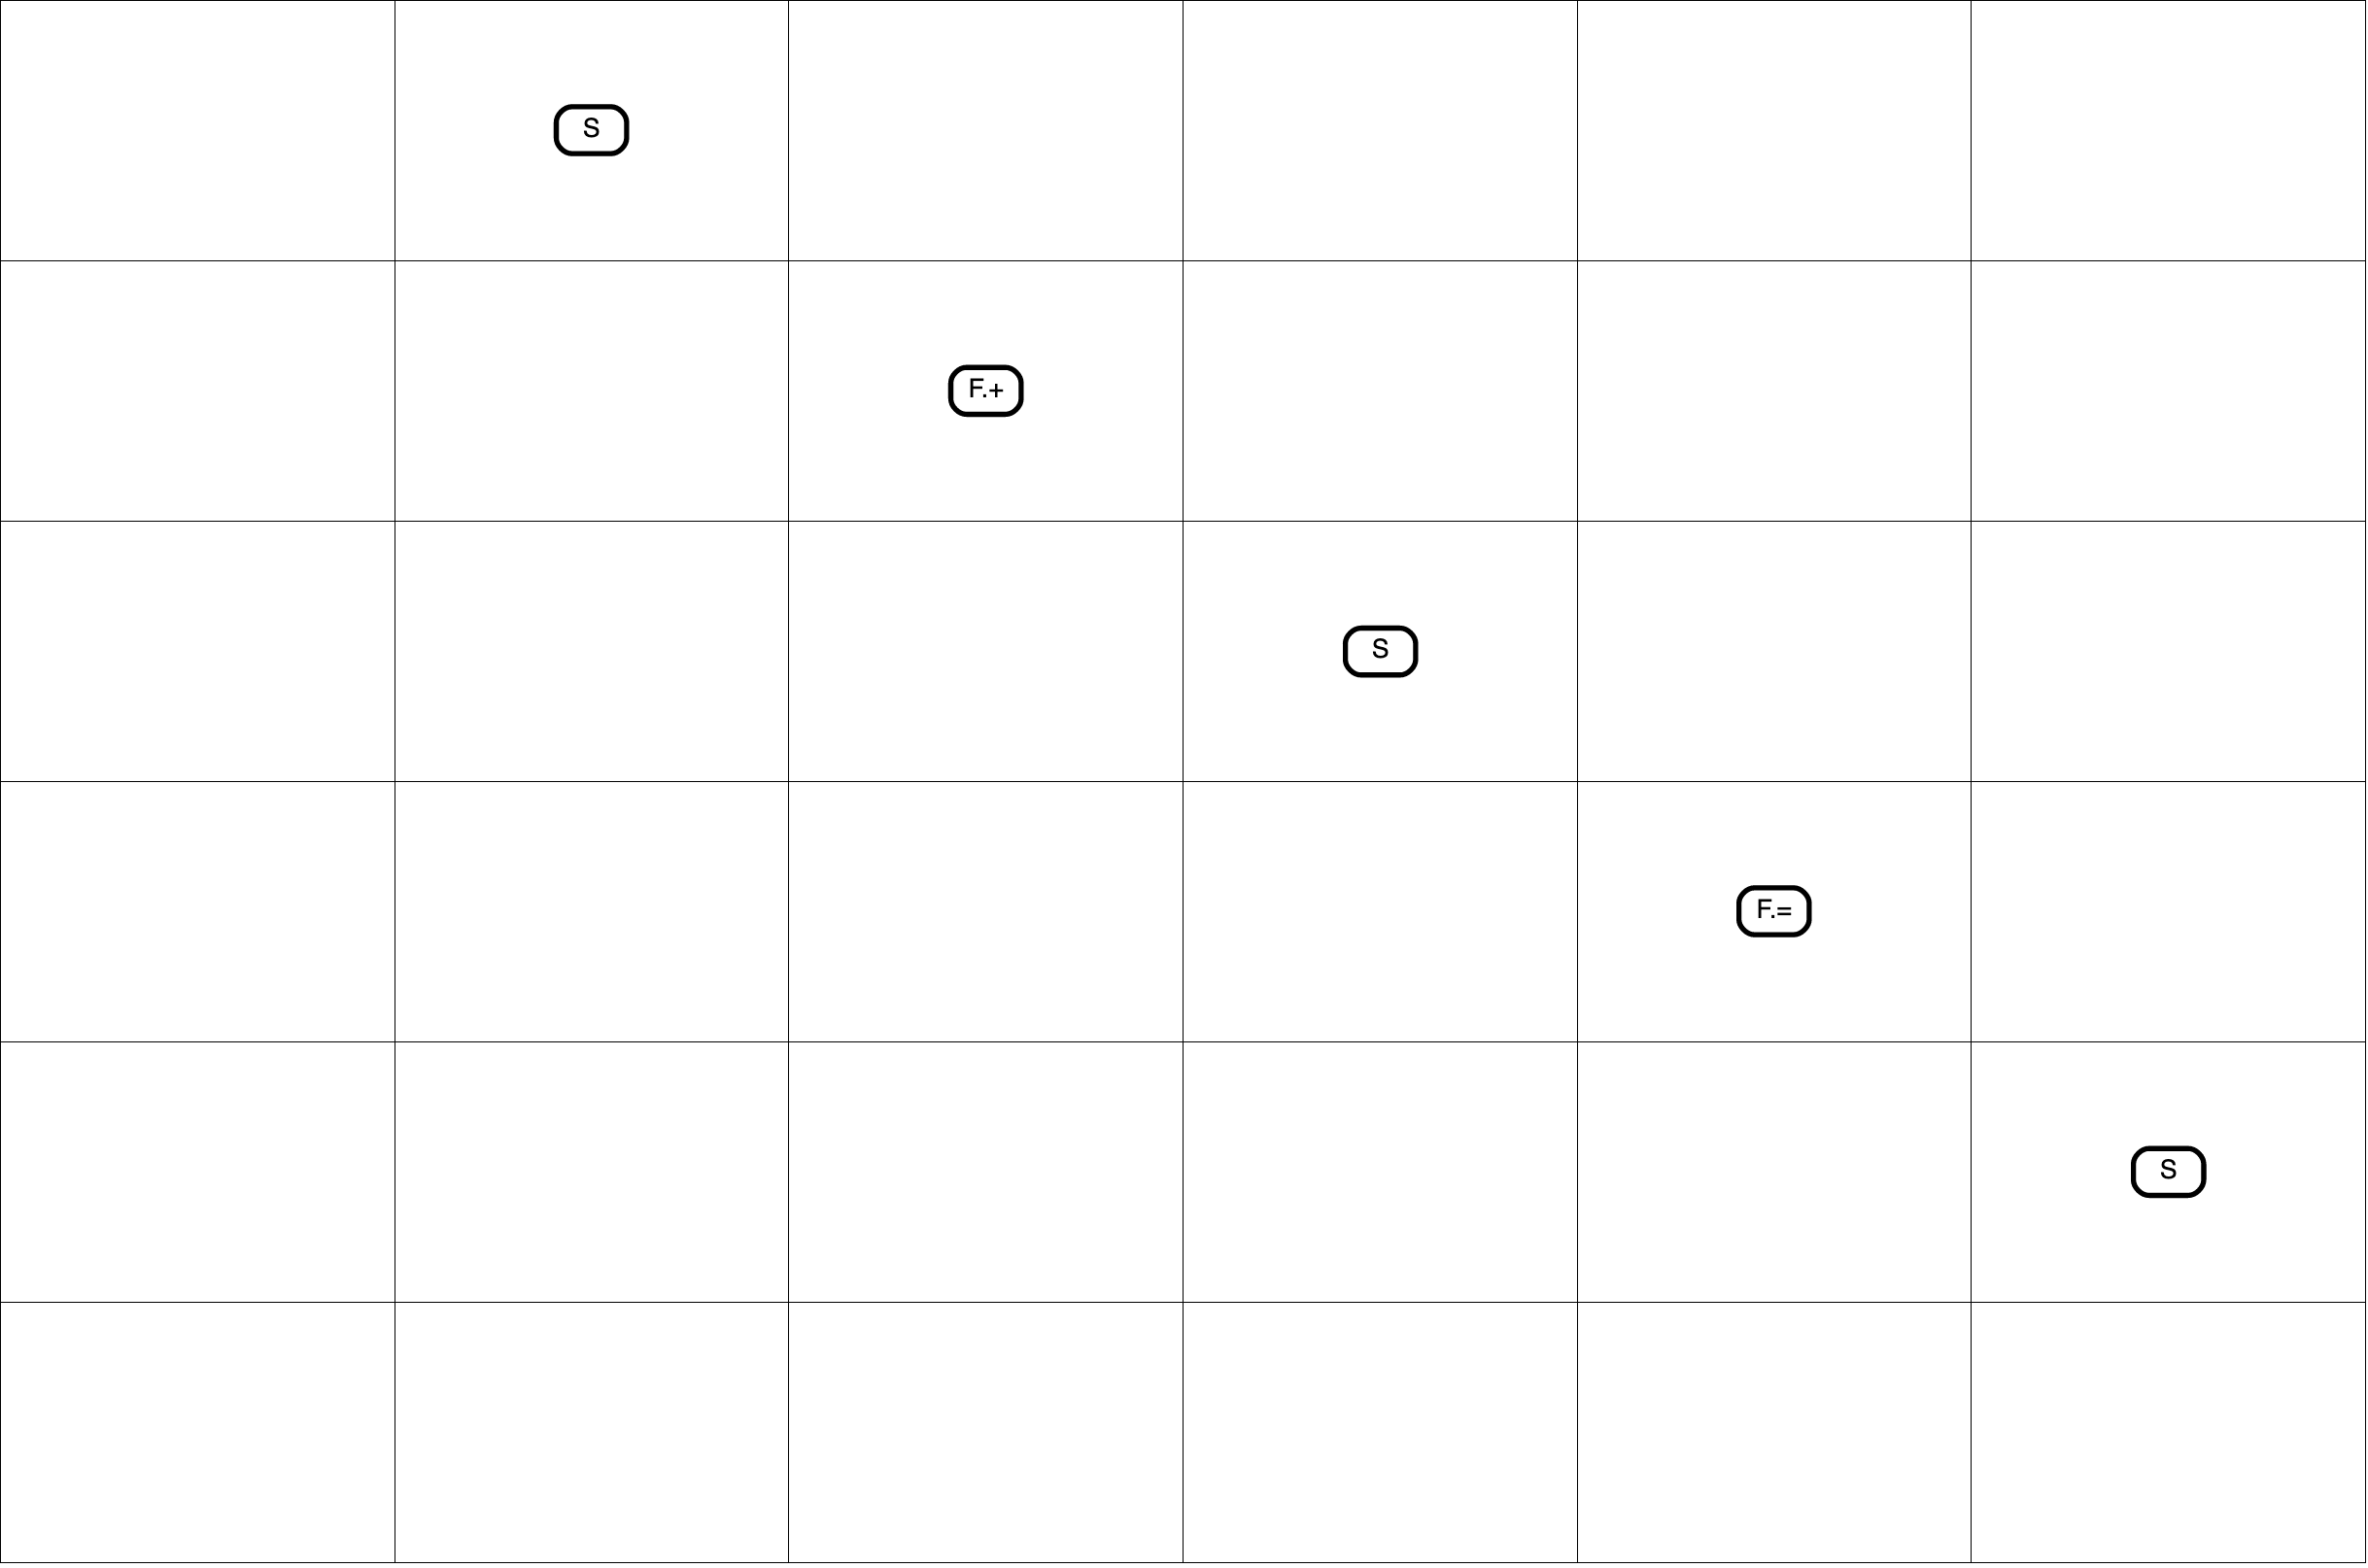
\includegraphics[width=3.305cm]{../figures/parse1.png}
    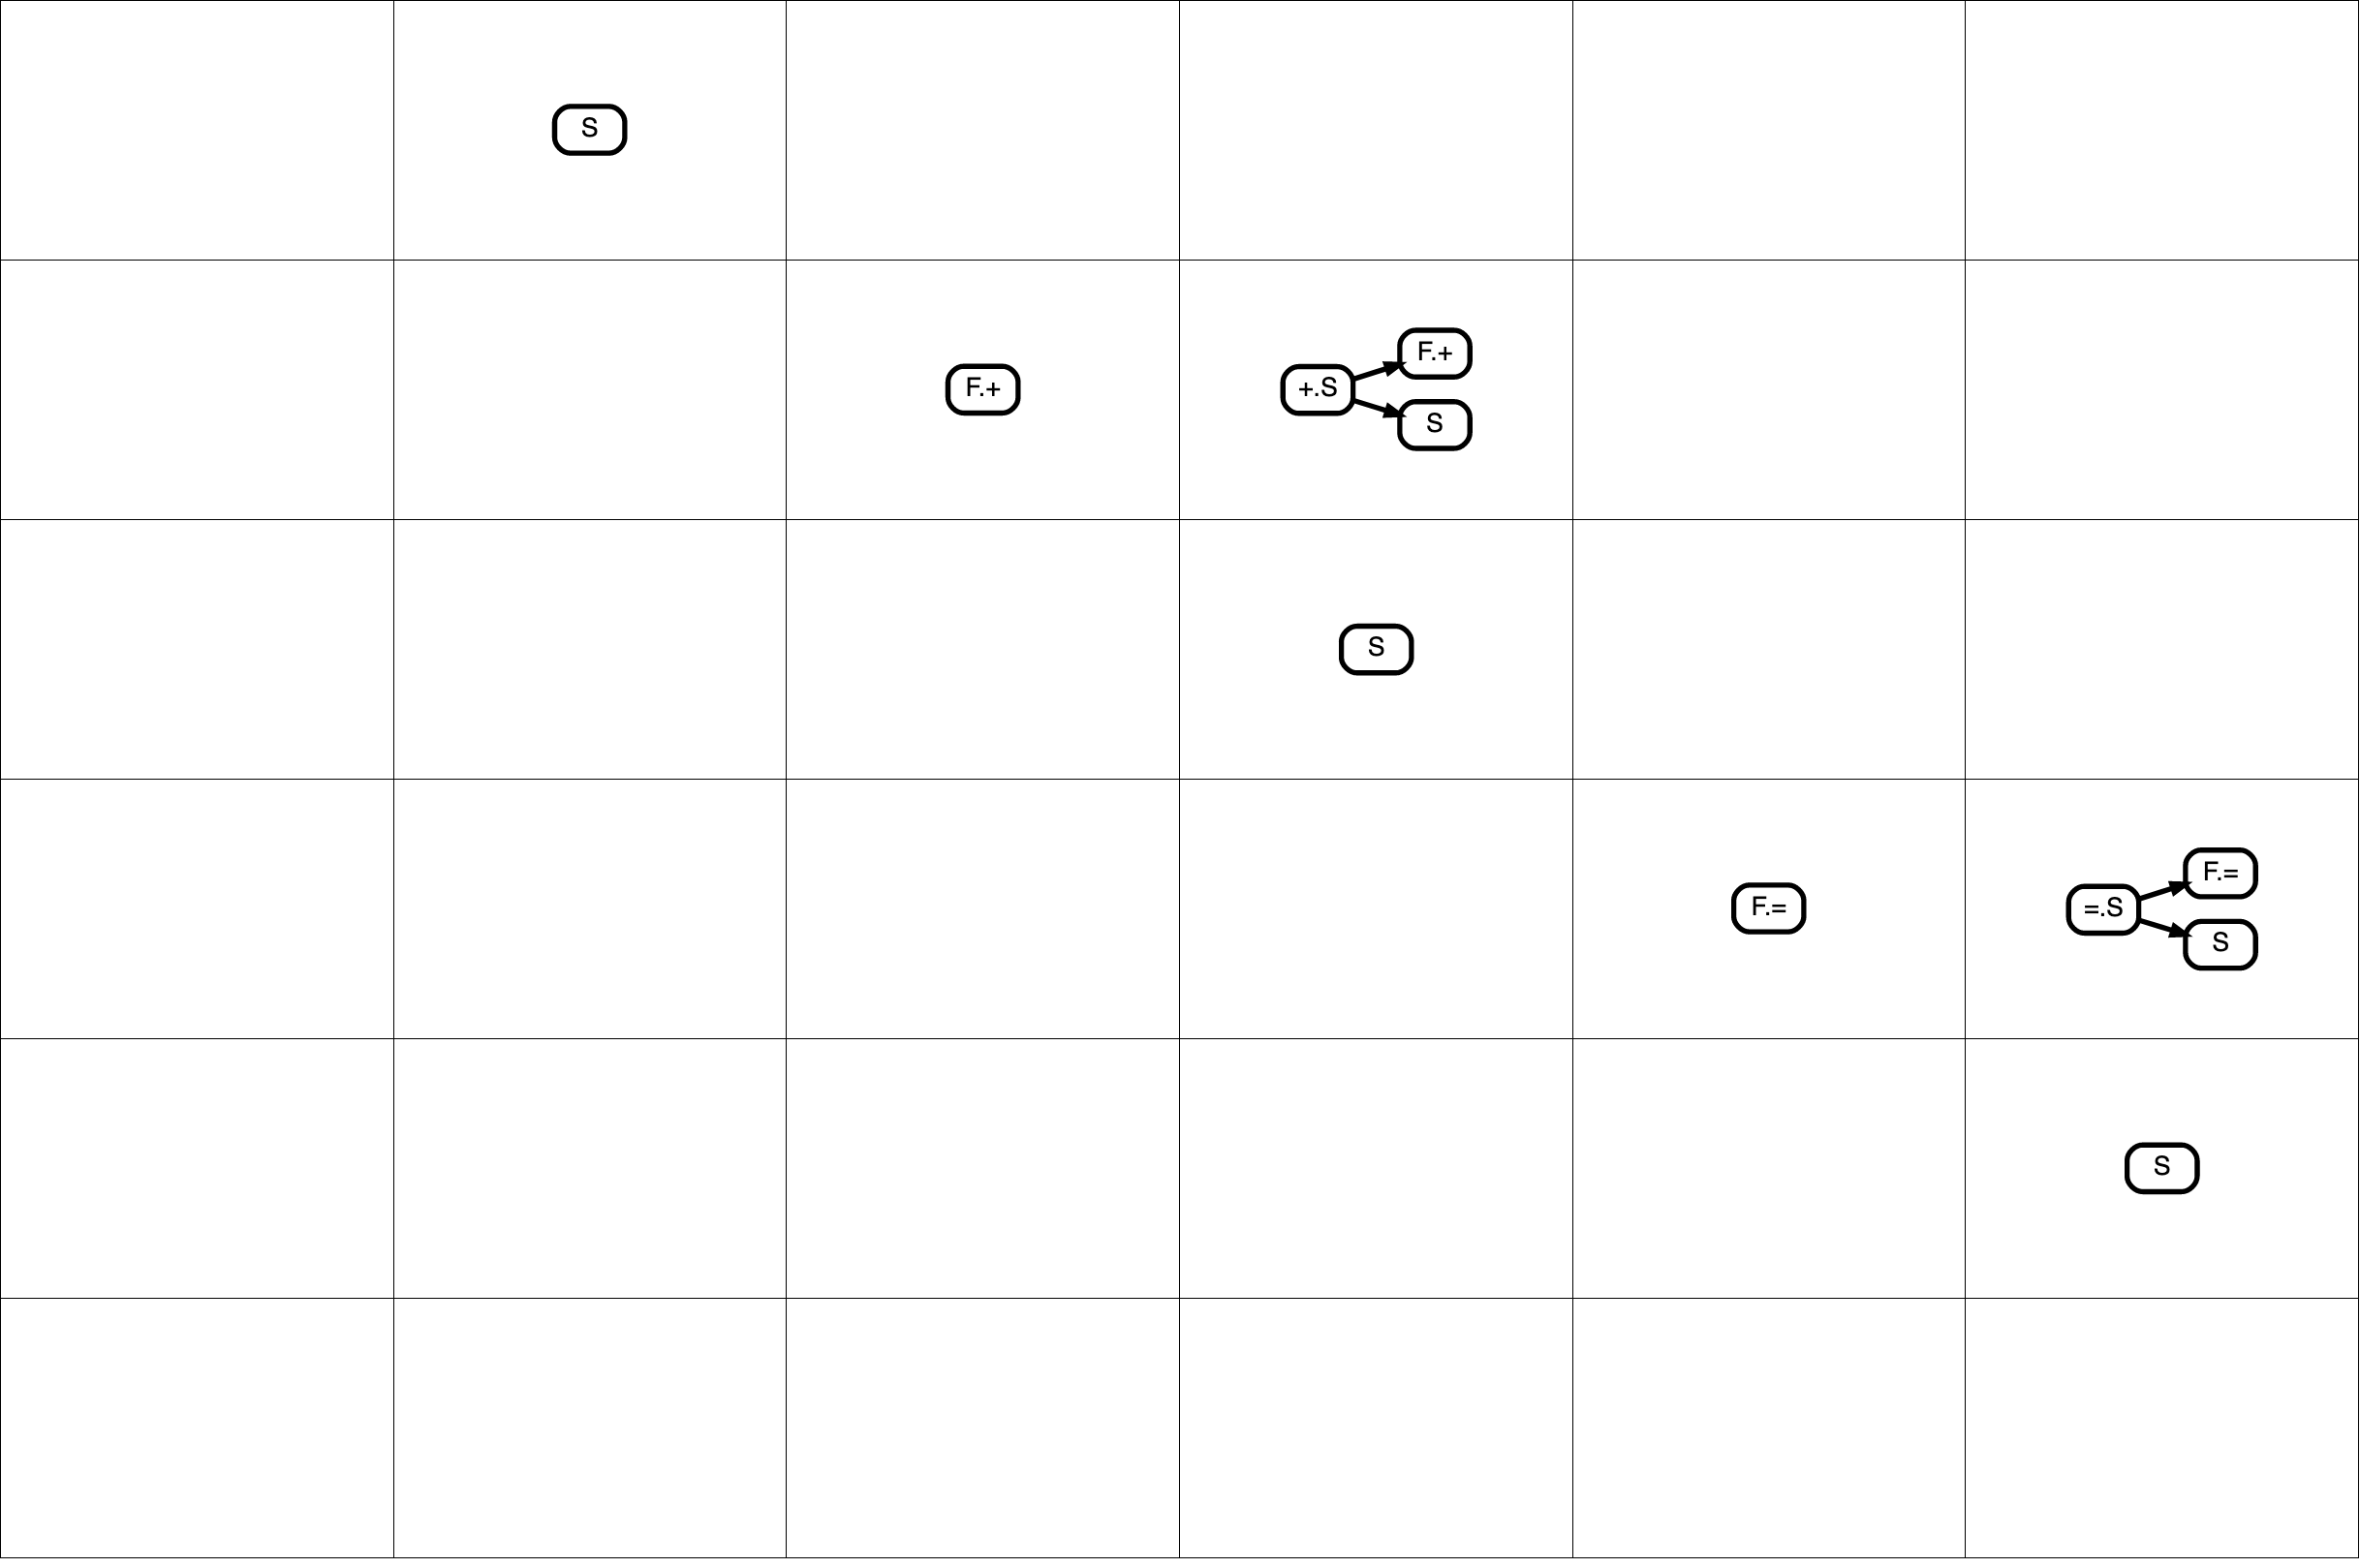
\includegraphics[width=3.298cm]{../figures/parse2.png}
    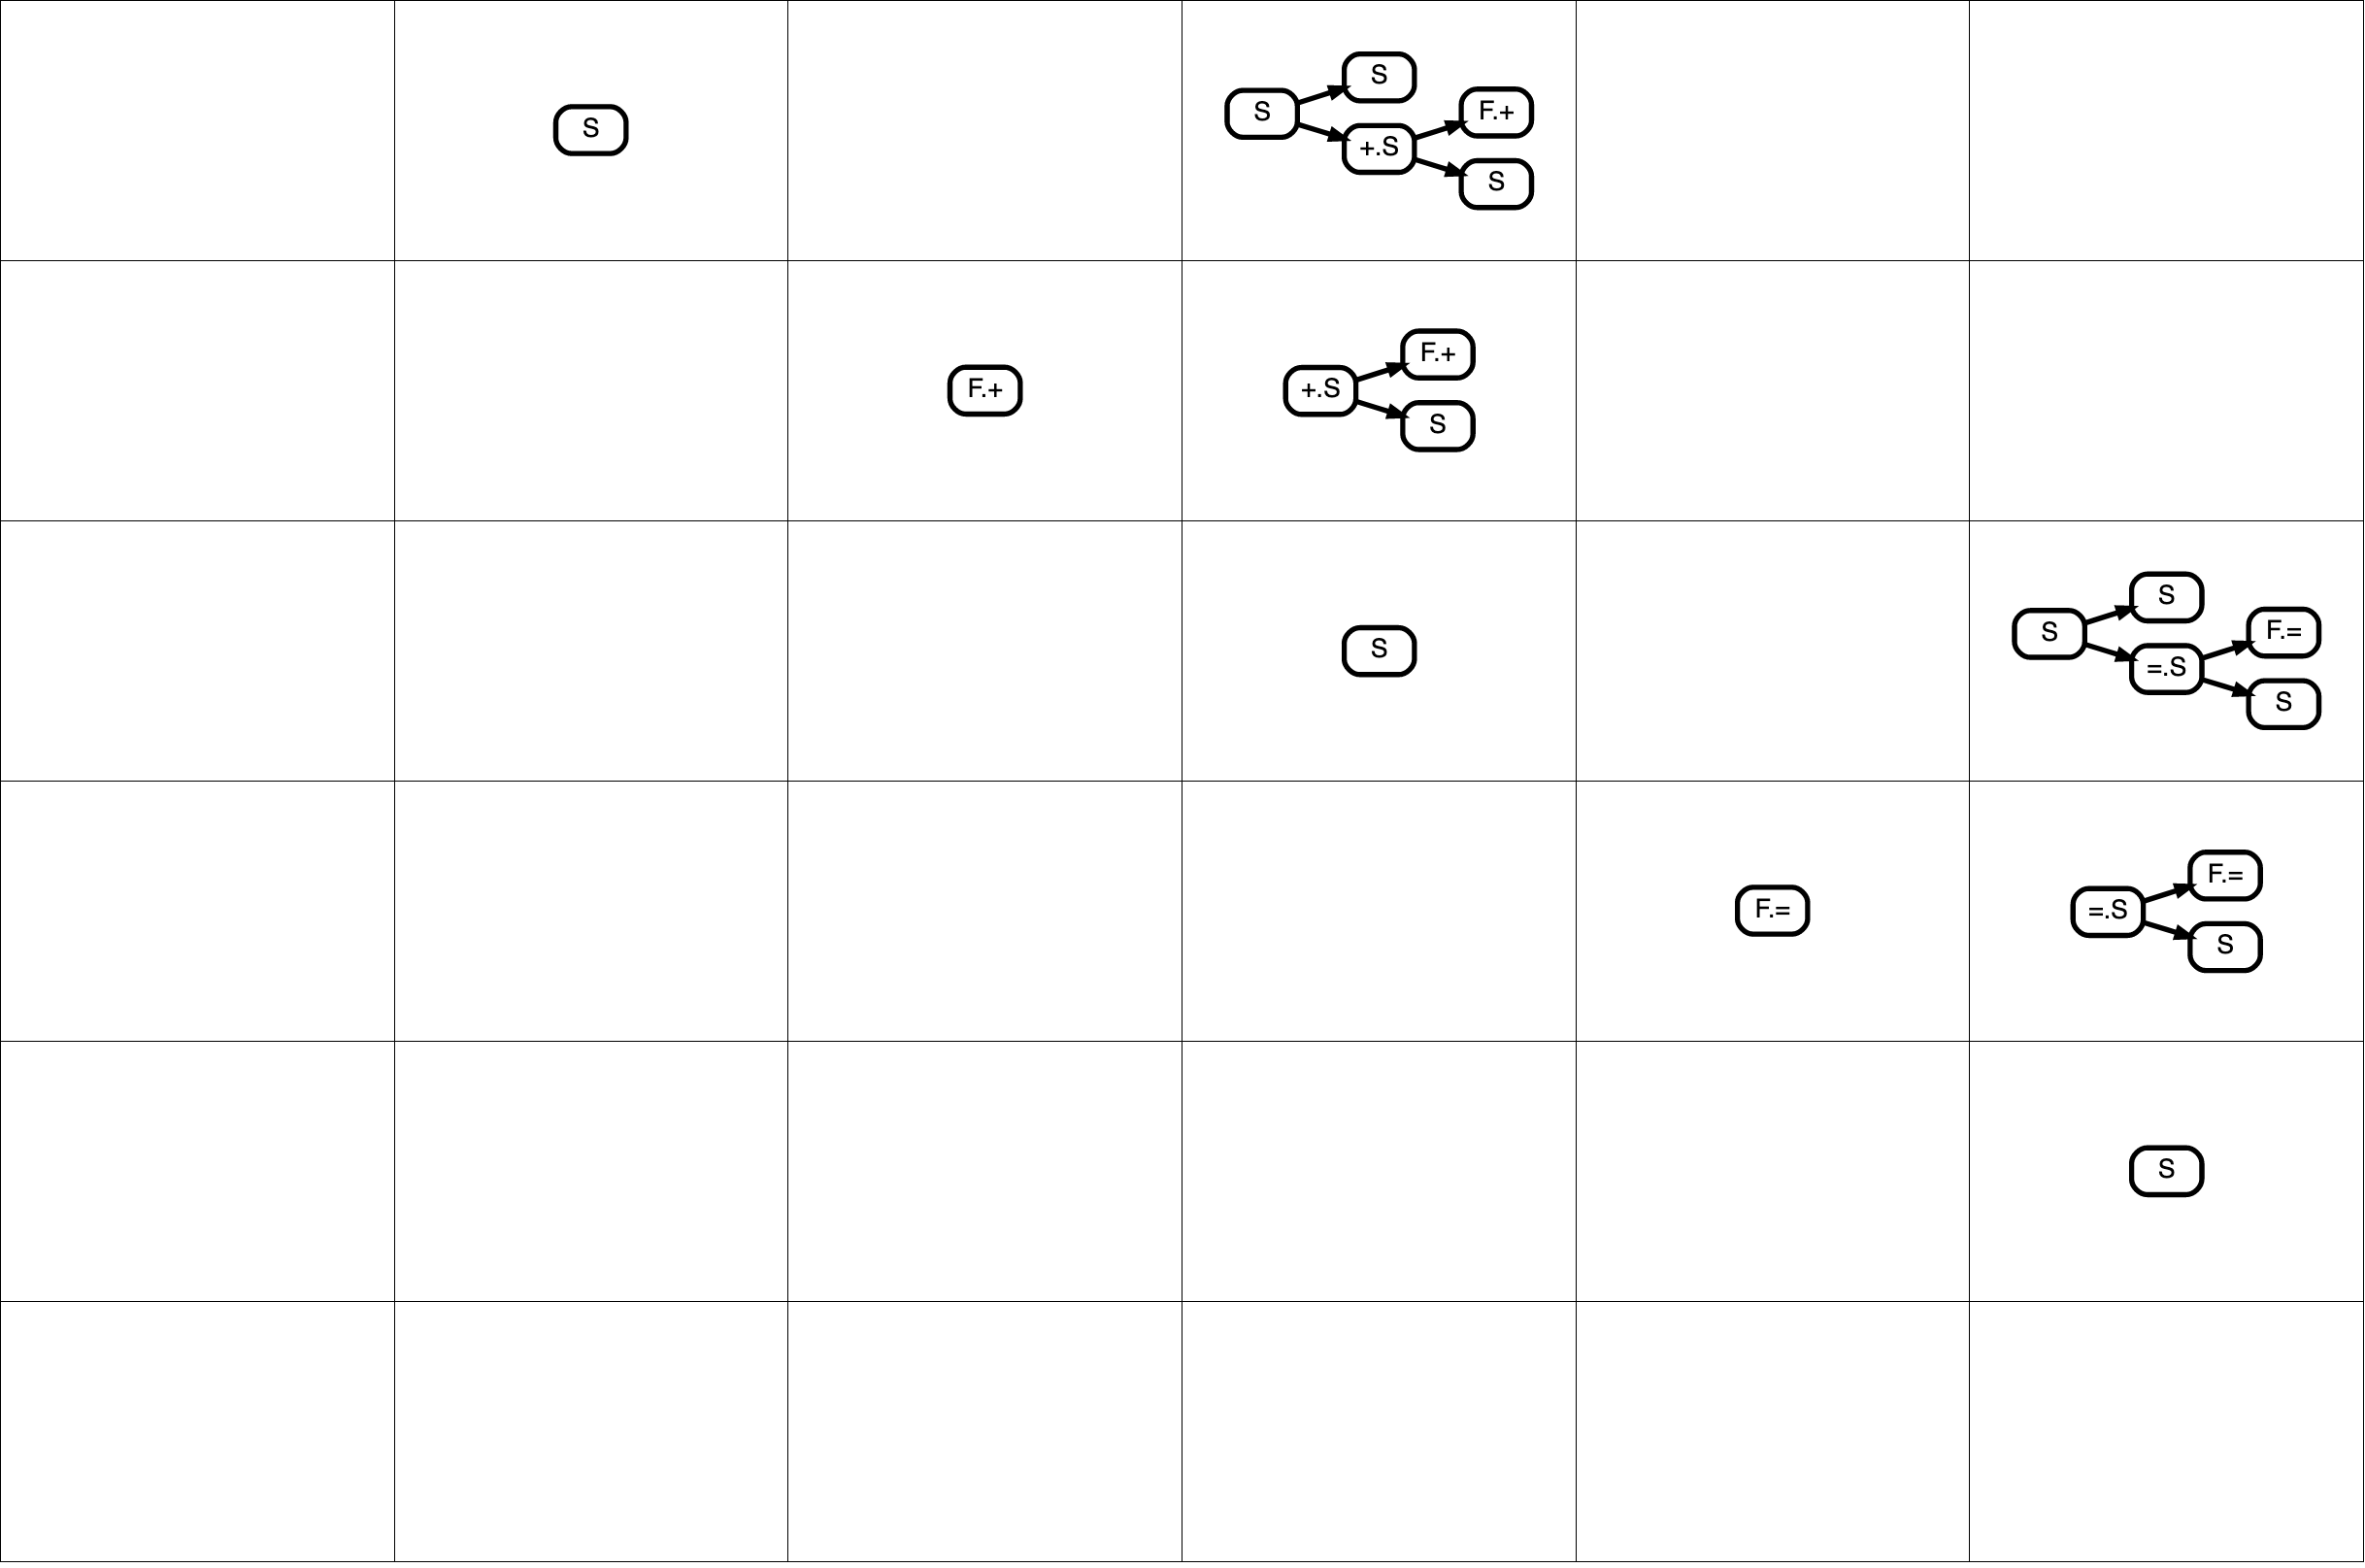
\includegraphics[width=3.3cm]{../figures/parse3.png}
    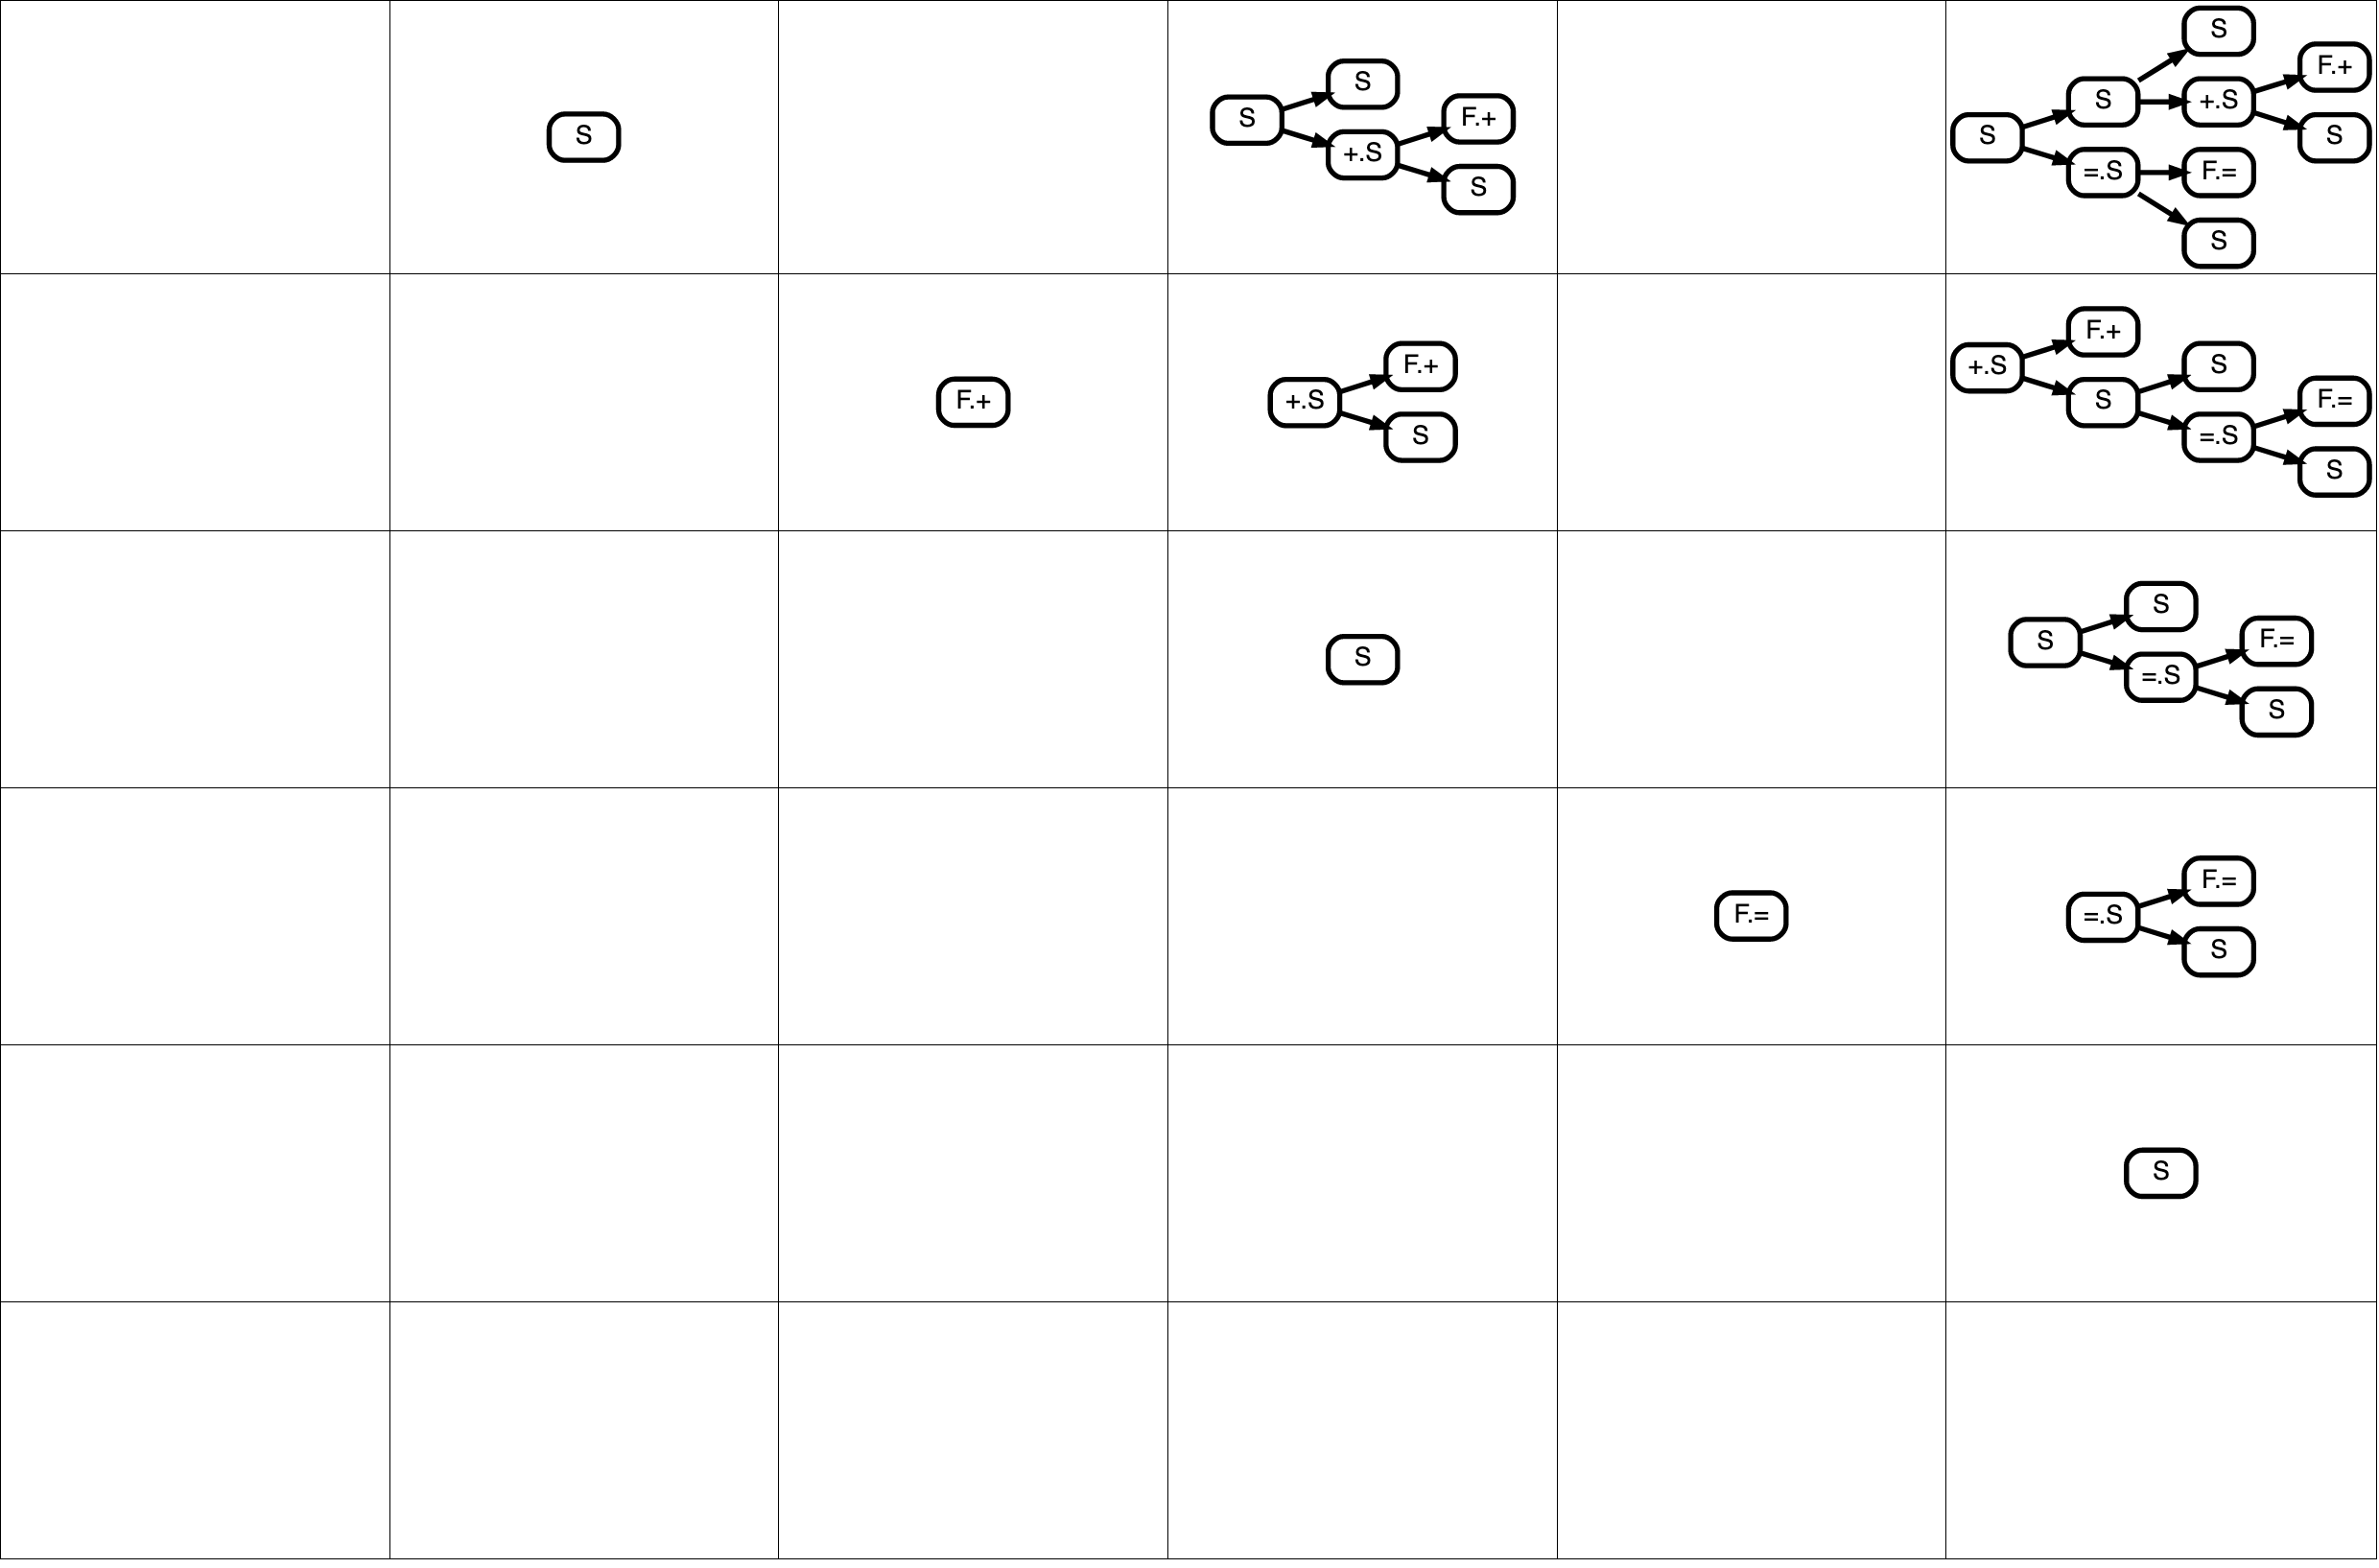
\includegraphics[width=3.32cm]{../figures/parse4.png}
  \caption{The parse forest for the string $S + S = S$ is constructed incrementally by computing $M_\sigma^2 + M_\sigma = M_\sigma$.}% Each iteration computes a single diagonal of the matrix by computing the dot product of the row-wise entries to the left and columnar entiries beneath it, and the process terminates when a fixpoint is reached.}
\end{figure}

For valid strings, the fixpoint search is sure to converge in at most $|\sigma| - 1$ steps, as each iteration will solve for a single diagonal of the matrix. Matrix entries may each contain up to $|V_\varepsilon|$ rooted subtrees, although in practice, this is typically much smaller for unambiguous grammars. If the string is invalid, the algorithm produces a set of admissible corrections, alongside their CSTs. An interesting consequence of repairing with a SAT solver is that we can directly encode matrix idempotency $[\mathcal{M}_\sigma=\mathcal{M}_\sigma^2]$, instead of solving Valiant's fixpoint $M_\sigma = M_\sigma + M^2_\sigma$.

\subsection{Incrementalization}\label{sec:incrementalization}

\begin{wrapfigure}{r}{0.4\textwidth}
  \vspace{-13pt}
  \resizebox{.4\textwidth}{!}{\begin{tabular}{ c c c c c }
  \scalebox{0.32}{\mkTrellisAppend{7}} & & \scalebox{0.32}{\mkTrellisInsert{6}}         & & \scalebox{0.32}{\mkTrellisInsert{7}}         \\
  Append                               & & Delete                                       & & Insert                                       \\
  $\mathcal{O}(n+1)$                   & & $\mathcal{O}\left(\frac{1}{4}(n-1)^2\right)$ & & $\mathcal{O}\left(\frac{1}{4}(n+1)^2\right)$ \\
\end{tabular}}
  \caption{Incremental reparsing only requires computing submatrices affected by an edit.}
  \label{fig:incremental}
\end{wrapfigure}

When a parsed string is altered, we can reuse prior work by only recomputing affected submatrices, yielding a reparser whose complexity is location-dependent, i.e., at worst quadratic in terms of $|\Sigma^*|$ assuming $\mathcal{O}(1)$ cost for each CNF-nonterminal subset join, $V_1'\otimes V_2'$. Letting shaded nodes represent observed or bound variables and unshaded nodes as free variables, we depict the worst-case post-editing state of the parse trellis in Fig.~\ref{fig:incremental}.

The problem of incremental parsing is closely related to \textit{dynamic matrix inversion} in the linear algebra setting, and \textit{incremental transitive closure} with vertex updates in the graph setting. By carefully encoding the matrix relation from \S\ref{sec:matrix} and employing an incremental SAT solver, we can gradually update SAT constraints as new keystrokes are received to eliminate redundancy.

%We can use an incremental SAT solver to encode the constraints. To do so, we encode the matrix equivalence relation and use the incremental SAT solver to update the constraints as new keystrokes are received. The incremental SAT solver will eliminate redundancy as it is introduced. Once a solution is found, we can use the algorithm from \S\ref{sec:denormalization} to recover the parse tree, then introduce a new constraint to block the solution and continue searching for other solutions.

\subsection{Error recovery}\label{sec:error_recovery}

\begin{wrapfigure}{R}{0.4\textwidth}
  \vspace{-20pt}
  \resizebox{0.4\textwidth}{!}{\[
  \mathbf{M}^* = \begin{pNiceArray}{ccccccc}[margin, extra-margin=2pt,colortbl-like, xdots/line-style=loosely dotted]
                   \tikzmark{a} & \tikzmark{k}  & \tikzmark{b} & \tikzmark{m} & \tikzmark{c} & \tikzmark{q} & \tikzmark{d} \\
                   \vno & \tikzmark{l}  &              & \tikzmark{n} &              & \tikzmark{r} & \tikzmark{w} \\
                   \vdd & \ddd          & \tikzmark{e} & \tikzmark{o} & \tikzmark{f} & \tikzmark{s} & \tikzmark{g} \\
                   &               &              & \tikzmark{p} &              & \tikzmark{t} & \tikzmark{x} \\
                   &               &              &              & \tikzmark{h} & \tikzmark{u} & \tikzmark{i} \\
                   &               &              &              &              & \tikzmark{v} &              \\
                   \vno & \cdd          &              &              &              & \vno         & \tikzmark{j}
  \end{pNiceArray}
  \begin{tikzpicture}[overlay, remember picture, blubr/.style={-,blue}, redbr/.style={-,red}, grnbr/.style={-,green}]
    \draw [grnbr] ({pic cs:l}) to ({pic cs:r});
    \draw [grnbr] ({pic cs:v}) to ({pic cs:r});
    \draw [grnbr] ({pic cs:r}) to ({pic cs:w});
    \draw [blubr] ({pic cs:a}) to ({pic cs:b});
    \draw [blubr] ({pic cs:e}) to ({pic cs:b});
    \draw [blubr] ({pic cs:h}) to ({pic cs:c});
    \draw [blubr] ({pic cs:b}) to ({pic cs:c});
    \draw [blubr] ({pic cs:c}) to ({pic cs:d});
    \draw [redbr] ({pic cs:h}) to ({pic cs:i});
    \draw [redbr] ({pic cs:j}) to ({pic cs:i});
    \draw [redbr] ({pic cs:e}) to ({pic cs:g});
    \draw [redbr] ({pic cs:i}) to ({pic cs:g});
    \draw [redbr] ({pic cs:g}) to ({pic cs:d});
  \end{tikzpicture}\Rightarrow
  \left\{\begin{pNiceArray}{ccccccc}[margin, extra-margin=2pt,colortbl-like, xdots/line-style=loosely dotted]
           \tikzmark{a1} & \tikzmark{k1}  & \tikzmark{b1} & \tikzmark{m1} & \tikzmark{c1} & \tikzmark{q1} & \tikzmark{d1} \\
           \vno          & \tikzmark{l1}  &               & \tikzmark{n1} &               & \tikzmark{r1} & \tikzmark{w1} \\
           \vdd          & \ddd           & \tikzmark{e1} & \tikzmark{o1} & \tikzmark{f1} & \tikzmark{s1} & \tikzmark{g1} \\
           &                &               & \tikzmark{p1} &               & \tikzmark{t1} & \tikzmark{x1} \\
           &                &               &               & \tikzmark{h1} & \tikzmark{u1} & \tikzmark{i1} \\
           &                &               &               &               & \tikzmark{v1} &              \\
           \vno          & \cdd           &               &               &               & \vno          & \tikzmark{j1}
  \end{pNiceArray}
  \begin{tikzpicture}[overlay, remember picture, redbr/.style={-,red}]
    \draw [redbr] ({pic cs:a1}) to ({pic cs:d1});
    \draw [redbr] ({pic cs:h1}) to ({pic cs:i1});
    \draw [redbr] ({pic cs:j1}) to ({pic cs:i1});
    \draw [redbr] ({pic cs:e1}) to ({pic cs:g1});
    \draw [redbr] ({pic cs:i1}) to ({pic cs:g1});
    \draw [redbr] ({pic cs:g1}) to ({pic cs:d1});
  \end{tikzpicture}_{\textstyle,}
  \begin{pNiceArray}{ccccccc}[margin, extra-margin=2pt,colortbl-like, xdots/line-style=loosely dotted]
    \tikzmark{a2} & \tikzmark{k2}  & \tikzmark{b2} & \tikzmark{m2} & \tikzmark{c2} & \tikzmark{q2} & \tikzmark{d2} \\
    \vno          & \tikzmark{l2}  &               & \tikzmark{n2} &               & \tikzmark{r2} & \tikzmark{w2} \\
    \vdd          & \ddd           & \tikzmark{e2} & \tikzmark{o2} & \tikzmark{f2} & \tikzmark{s2} & \tikzmark{g2} \\
    &                &               & \tikzmark{p2} &               & \tikzmark{t2} & \tikzmark{x2} \\
    &                &               &               & \tikzmark{h2} & \tikzmark{u2} & \tikzmark{i2} \\
    &                &               &               &               & \tikzmark{v2} &              \\
    \vno          & \cdd           &               &               &               & \vno          & \tikzmark{j2}
  \end{pNiceArray}
  \begin{tikzpicture}[overlay, remember picture, blubr/.style={-,blue}]
    \draw [blubr] ({pic cs:a2}) to ({pic cs:b2});
    \draw [blubr] ({pic cs:e2}) to ({pic cs:b2});
    \draw [blubr] ({pic cs:h2}) to ({pic cs:c2});
    \draw [blubr] ({pic cs:b2}) to ({pic cs:c2});
    \draw [blubr] ({pic cs:c2}) to ({pic cs:d2});
    \draw [blubr] ({pic cs:j2}) to ({pic cs:d2});
  \end{tikzpicture}_{\textstyle,}
  \begin{pNiceArray}{ccccccc}[margin, extra-margin=2pt,colortbl-like, xdots/line-style=loosely dotted]
    \tikzmark{a3} & \tikzmark{k3}  & \tikzmark{b3} & \tikzmark{m3} & \tikzmark{c3} & \tikzmark{q3} & \tikzmark{d3} \\
    \vno          & \tikzmark{l3}  &               & \tikzmark{n3} &               & \tikzmark{r3} & \tikzmark{w3} \\
    \vdd          & \ddd           & \tikzmark{e3} & \tikzmark{o3} & \tikzmark{f3} & \tikzmark{s3} & \tikzmark{g3} \\
    &                &               & \tikzmark{p3} &               & \tikzmark{t3} & \tikzmark{x3} \\
    &                &               &               & \tikzmark{h3} & \tikzmark{u3} & \tikzmark{i3} \\
    &                &               &               &               & \tikzmark{v3} &              \\
    \vno          & \cdd           &               &               &               & \vno          & \tikzmark{j3}
  \end{pNiceArray}
  \begin{tikzpicture}[overlay, remember picture, grnbr/.style={-,green}]
    \draw [grnbr] ({pic cs:l3}) to ({pic cs:r3});
    \draw [grnbr] ({pic cs:n3}) to ({pic cs:p3});
    \draw [grnbr] ({pic cs:v3}) to ({pic cs:r3});
    \draw [grnbr] ({pic cs:r3}) to ({pic cs:w3});
    \draw [grnbr] ({pic cs:j3}) to ({pic cs:d3});
    \draw [grnbr] ({pic cs:a3}) to ({pic cs:d3});
  \end{tikzpicture}\ldots\right\}
\]
}
  \caption{The matrix $M^*$ contains all admissible binary trees of a fixed breadth.}\label{fig:binary_trees}
  \begin{center}
  \resizebox{.35\textwidth}{!}{\hspace{-0.5cm}\begin{minipage}[l]{6cm}
    \[
      \begin{NiceMatrix}
        \leftarrow & \nse & \nsi & \nfi & \nfo & \nth & \ntw & \non & \leftarrow & \ppp \\
        &      & \ddd & \ddd & \ddd & \ddd & \ddd & \ddd & \ddd & \ppp \\
        \sigma_1^\shri & \cdd &      & A    &      &      &      &      &      & \ppp \\
        \vno & \ddd &  T_A & \vdd &      &      &      &      &      & \ppp \\
        \vdd & \ddd &      & \pcd & \cdd &      & B    &      &      & \ppp \\
        &      &      &      &      & T_B  & \vdd &      &      & \ppp \\
        &      &      &      &      &      & \pcd & \cdd &      & C    \\
        &      &      &      &      &      &      &      & T_C  & \vdd \\
        &      &      &      &      &      &      &      &      & \\
        &      &      &      &      &      &      &      &      & \\
        &      &      &      &      &      &      &      &      & \\
        &      &      &      &      &      &      &      & \ppp & \sigma_n^\shup \\
        \vno & \cdd &      &      &      &      &      &      & \vno &
      \end{NiceMatrix}
    \]
\end{minipage}
\hspace{1cm}
\begin{minipage}[l]{6cm}
  \begin{halftidyinput}
  (*@\err{\texttt{⊤ and ⊤ ! and ⊥ xor ⊤ ! ⊤ and ⊥}}\caret{ }@*)
  \end{halftidyinput}

  \begin{verbatim}
    Recovered 3 parseable leaves:
  \end{verbatim}
  \noindent\hspace{0.64cm}\emoji{herb}\hspace{1.70cm}\emoji{herb}\hspace{1.98cm}\emoji{herb}\vspace{-5pt}
  \begin{verbatim}
    └── ! [3]   └── and [4]   └── xor [6]
  \end{verbatim}

  \begin{verbatim}
    Recovered 2 parseable branches:
  \end{verbatim}
  \hspace{0.64cm}\emoji{herb}\hspace{2.51cm}\emoji{herb}\vspace{-5pt}
  \begin{verbatim}
    └── S [0..2]     └── S [8..11]
        ├── ⊤ [0]        ├── S [8..9]
        ├── and [1]      │   ├── ! [8]
        └── ⊤ [2]        │   └── ⊤ [9]
                         ├── and [10]
                         └── ⊥ [11]
  \end{verbatim}
\end{minipage}}
  \end{center}
  \caption{We can recover the partial subtrees for invalid strings by inspecting $M^*$.}\label{fig:peaks}
\end{wrapfigure}

Not only is Tidyparse capable of suggesting repairs to invalid strings, it can also return partial trees for those same strings, which is often helpful for debugging purposes. Unlike LL- and LR-style parsers which require special rules for error recovery, Tidyparse can simply analyze the structure of $M^*$ to recover parse branches. If $S \notin  \Lambda^*_\sigma$, the upper triangular entries of $M^*$ will take the form of a jagged-shaped ridge whose peaks signify the roots of maximally-parsable substrings $\hat{\sigma}_{i, j}$.

These branches are located on peaks of the upper triangular (UT) matrix ridge. As depicted in Fig.~\ref{fig:peaks}, we traverse the peaks by decreasing elevation to collect partial AST branches and display the highest nonoverlapping branches, in this case $T_C$ and $T_A$ to the user, to help them diagnose the parsing error and manually repair it.


%When completing a bounded-width string, one finds it is often convenient to admit nonterminal stubs, representing unexpanded subexpressions. To enable this functionality, we introduce a synthetic production for each $v \in V$ using the $\langle\cdot\rangle\textsc{-int}$ rule. Users can interactively build up a complex expression by placing the caret over a stub, then pressing \keys{\ctrl + \SPACE}:
%
%\begin{tcolorbox}[left skip=0.7cm,
%top=0.1cm,
%middle=0mm,
%boxsep=0mm,
%underlay unbroken and first={%
%\path[draw=none] (interior.north west) rectangle node[white]{
\includegraphics[width=4mm]{../figures/tidyparse_logo.png}} ([xshift=-10mm,yshift=-9mm]interior.north west);
%}]
%\begin{lstlisting} [language=tidy, basicstyle=\ttfamily\small, escapeinside={(*@}{@*)}]
%false or ! true or <(*@\caret{S}@*)> and <S> or <S>
%\end{lstlisting}
%\tcblower
%\begin{lstlisting} [language=tidy, basicstyle=\ttfamily\small, escapeinside={(*@}{@*)}]
%1.) false or ! true or (*@\hlorange{true}@*) and <S> or <S>
%2.) false or ! true or (*@\hlorange{false}@*) and <S> or <S>
%3.) false or ! true or (*@\hlorange{!}@*) (*@\hlorange{<S>}@*) and <S> or <S>
%4.) false or ! true or (*@\hlorange{<S>}@*) (*@\hlorange{and}@*) (*@\hlorange{<S>}@*) and <S> or <S>
%5.) false or ! true or (*@\hlorange{<S>}@*) (*@\hlorange{or}@*) (*@\hlorange{<S>}@*) and <S> or <S>
%...
%\end{lstlisting}
%\end{tcolorbox}
%
%\noindent This functionality can also be useful inside a completion, which might be expanded as follows:
%
%\begin{tcolorbox}[left skip=0.7cm,
%top=0.1cm,
%middle=0mm,
%boxsep=0mm,
%underlay unbroken and first={%
%\path[draw=none] (interior.north west) rectangle node[white]{
\includegraphics[width=4mm]{../figures/tidyparse_logo.png}} ([xshift=-10mm,yshift=-9mm]interior.north west);
%}]
%\begin{lstlisting} [language=tidy, basicstyle=\ttfamily\small, escapeinside={(*@}{@*)}]
%if <Vexp> _ _ _ _ _(*@\caret{ }@*)
%\end{lstlisting}
%\tcblower
%\begin{lstlisting} [language=tidy, basicstyle=\ttfamily\small, escapeinside={(*@}{@*)}]
%1.) if (*@\hlorange{map}@*) X then <Vexp> else <Vexp>
%2.) if (*@\hlorange{uncurry}@*) X then <Vexp> else <Vexp>
%3.) if (*@\hlorange{foldright}@*) X then <Vexp> else <Vexp>
%...
%\end{lstlisting}
%\end{tcolorbox}

\pagebreak\section{Usage examples}\label{sec:examples}


Suppose we are given the following context-free grammar:

\begin{wholetidyinput}
S -> S and S | S xor S | ( S ) | true | false | ! S(*@\caret{ }@*)
\end{wholetidyinput}

\noindent For reasons that will become clear in Sec.~\ref{sec:matrix}, this will automatically be rewritten into the grammar:

\begin{verbatim}
 F.! → !     S.) → S F.)  and.S → F.and S   S → F.! S     S → false    S → S ε+
 F.( → (   F.xor → xor    xor.S → F.xor S   S → S and.S   S → true    ε+ → ε
 F.) → )   F.and → and        S → S xor.S   S → F.( S.)   S → <S>     ε+ → ε+ ε+
\end{verbatim}

%\noindent We can visualize the CFG as either a graph or a matrix:
%
%\begin{figure}[H]
%    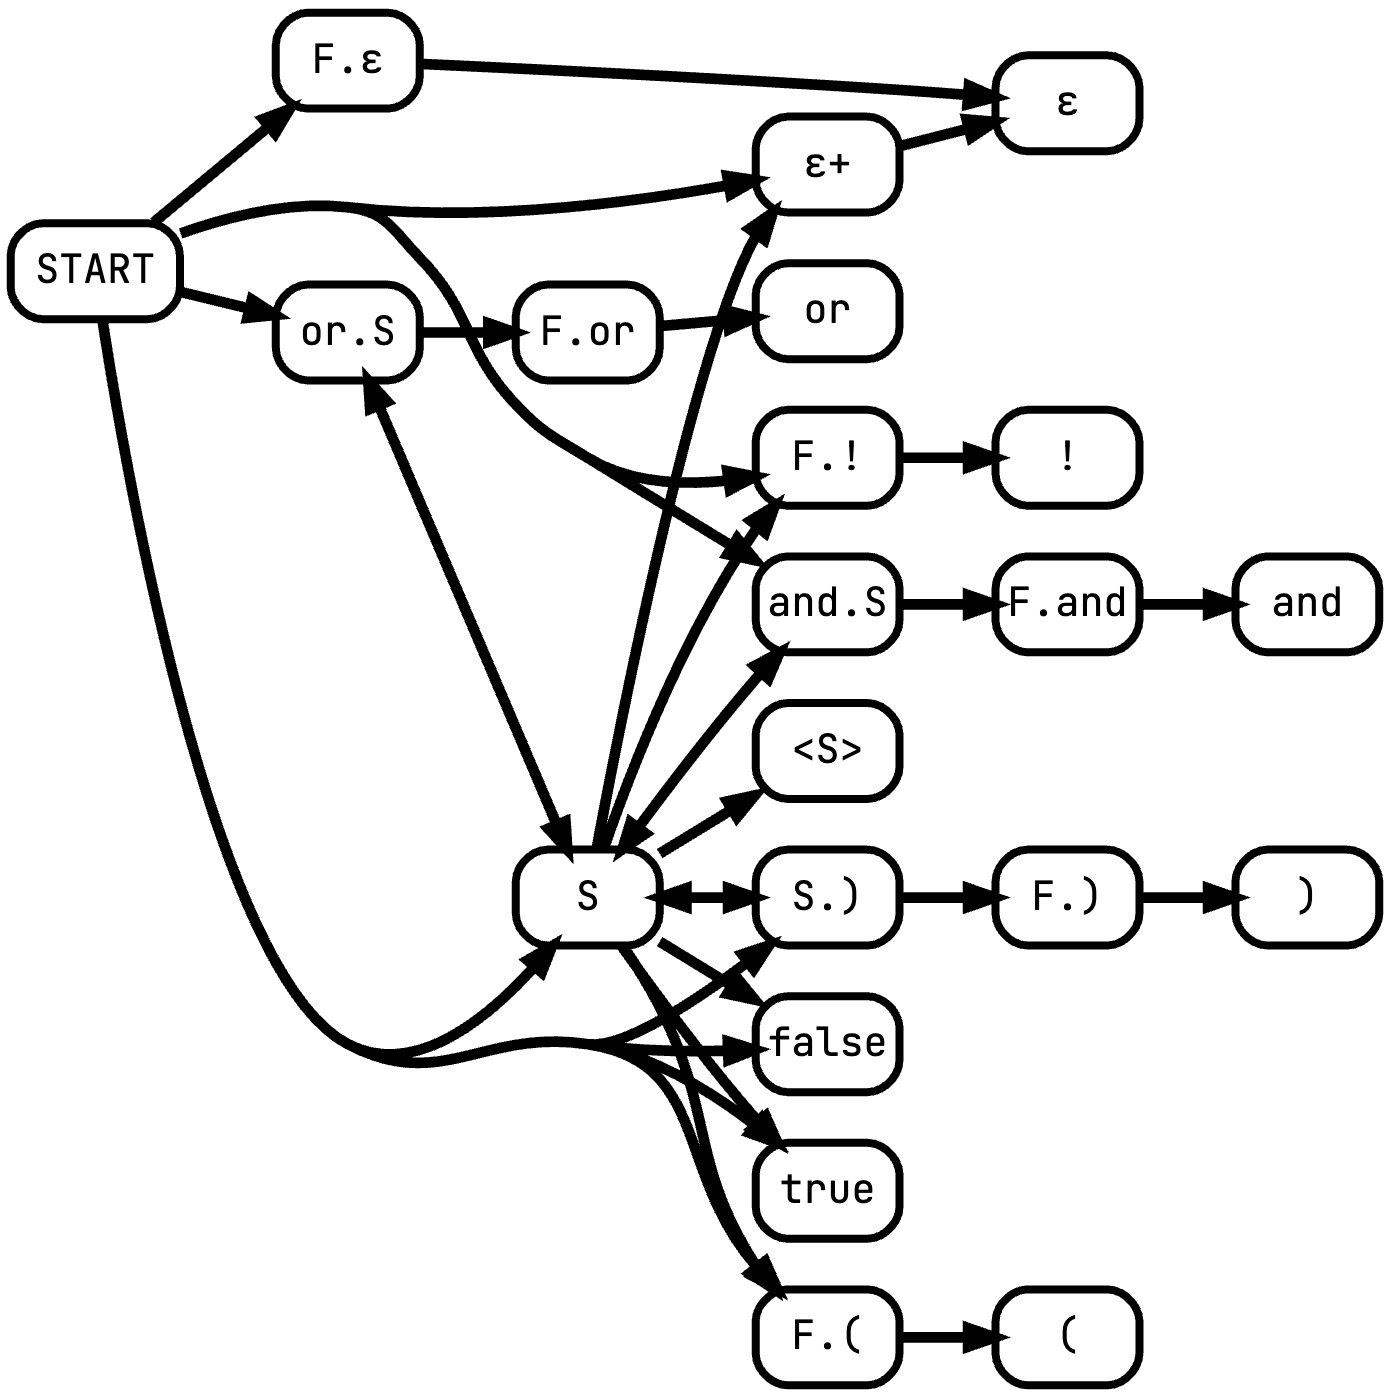
\includegraphics[width=3.5cm]{../figures/bool_arith_cfg_graph.png}
%    \hspace{20pt}
%    \includegraphics[width=3.5cm]{../figures/bool_arith_cfg_mat.bmp}
%\end{figure}

\noindent Given a string containing holes, our tool will return several completions in a few milliseconds:

\begin{tcolorbox}[left skip=0.7cm,
top=0.1cm,
middle=0mm,
boxsep=0mm,
underlay unbroken and first={%
    \path[draw=none] (interior.north west) rectangle node[white]{
\includegraphics[width=4mm]{../figures/tidyparse_logo.png}} ([xshift=-10mm,yshift=-9mm]interior.north west);
}]
  \begin{lstlisting} [language=tidy, basicstyle=\ttfamily\small, escapeinside={(*@}{@*)}]
true _ _ _ ( false _ ( _ _ _ _ ! _ _ ) _ _ _ _(*@\caret{ }@*)
  \end{lstlisting}
  \tcblower
  \begin{lstlisting} [language=tidy, basicstyle=\ttfamily\small, escapeinside={(*@}{@*)}]
true (*@\hlorange{xor}@*) (*@\hlorange{!}@*) ( false (*@\hlorange{xor}@*) ( <S> (*@\hlorange{)}@*) or ! (*@\hlorange{<S>}@*) ) (*@\hlorange{xor}@*) (*@\hlorange{<S>}@*)
true (*@\hlorange{xor}@*) (*@\hlorange{!}@*) ( false (*@\hlorange{and}@*) ( <S> (*@\hlorange{)}@*) or ! (*@\hlorange{<S>}@*) ) (*@\hlorange{xor}@*) (*@\hlorange{<S>}@*)
true (*@\hlorange{xor}@*) (*@\hlorange{!}@*) ( false (*@\hlorange{and}@*) ( <S> (*@\hlorange{)}@*) and ! (*@\hlorange{<S>}@*) ) (*@\hlorange{xor}@*) (*@\hlorange{<S>}@*)
true (*@\hlorange{xor}@*) (*@\hlorange{!}@*) ( false (*@\hlorange{and}@*) ( <S> (*@\hlorange{)}@*) and ! (*@\hlorange{<S>}@*) ) (*@\hlorange{and}@*) (*@\hlorange{<S>}@*)
...
  \end{lstlisting}
\end{tcolorbox}

\noindent Similarly, if provided with a string containing various errors, it will return several suggestions how to fix it, where \hlgreen{green} is insertion, \hlorange{orange} is substitution and \hlred{red} is deletion.

\begin{tcolorbox}[left skip=0.7cm,
top=0.1cm,
middle=0mm,
boxsep=0mm,
underlay unbroken and first={%
    \path[draw=none] (interior.north west) rectangle node[white]{
\includegraphics[width=4mm]{../figures/tidyparse_logo.png}} ([xshift=-10mm,yshift=-9mm]interior.north west);
}]
\begin{lstlisting} [language=tidy, basicstyle=\ttfamily\small, escapeinside={(*@}{@*)}]
true and ( false or and true false(*@\caret{ }@*)
\end{lstlisting}
\tcblower
\begin{lstlisting} [language=tidy, basicstyle=\ttfamily\small, escapeinside={(*@}{@*)}]
1.) true and ( false or (*@\hlorange{!}@*) true (*@\hlorange{)}@*)
2.) true and ( false or (*@\hlgreen{<S>}@*) and true (*@\hlorange{)}@*)
3.) true and ( false or (*@\hlorange{(}@*) true (*@\hlorange{)}@*) (*@\hlgreen{)}@*)
...
9.) true and ( false or (*@\hlgreen{!}@*) (*@\hlgreen{<S>}@*) (*@\hlgreen{)}@*) and true (*@\hlred{false} @*)
\end{lstlisting}
\end{tcolorbox}

\noindent Given an invalid string, the tool will first map the string to a coarsened version and generate edits:

\hspace{-0.3cm}\begin{minipage}[t]{0.5\textwidth}
\begin{tcolorbox}[left skip=0.7cm,
top=0.1cm,
middle=0mm,
boxsep=0mm,
underlay unbroken and first={%
  \path[draw=none] (interior.north west) rectangle node[white]{
\includegraphics[width=4mm]{../figures/tidyparse_logo.png}} ([xshift=-10mm,yshift=-9mm]interior.north west);
}]
\begin{lstlisting} [language=tidy, basicstyle=\ttfamily\small, escapeinside={(*@}{@*)}]
v = [float(n for n in l.split(':')]
\end{lstlisting}
\tcblower
\begin{lstlisting} [language=tidy, basicstyle=\ttfamily\small, escapeinside={(*@}{@*)}]
v = [float(*@\hlred{(}@*)n for n in l.split(':')]
v = [float((*@\hlgreen{)}@*)n for n in l.split(':')]
v = [float((*@\hlorange{)}@*) for n in l.split(':')]
v = [float(n(*@\hlgreen{)}@*) for n in l.split(':')]
\end{lstlisting}
\end{tcolorbox}
\end{minipage}
\begin{minipage}[t]{0.5\textwidth}
\begin{tcolorbox}[left skip=0.7cm,
top=0.1cm,
middle=0mm,
boxsep=0mm,
underlay unbroken and first={%
  \path[draw=none] (interior.north west) rectangle node[white]{
\includegraphics[width=4mm]{../figures/tidyparse_logo.png}} ([xshift=-10mm,yshift=-9mm]interior.north west);
}]
\begin{lstlisting} [language=tidy, basicstyle=\ttfamily\small, escapeinside={(*@}{@*)}]
w = [ w ( w w w w w . w ( w ) ]
\end{lstlisting}
\tcblower
\begin{lstlisting} [language=tidy, basicstyle=\ttfamily\small, escapeinside={(*@}{@*)}]
w = [ w (*@\hlred{(}@*) w w w w w . w ( w ) ]
w = [ w ( (*@\hlgreen{)}@*) w w w w w . w ( w ) ]
w = [ w ( (*@\hlorange{)}@*) w w w w . w ( w ) ]
w = [ w ( w (*@\hlgreen{)}@*) w w w w . w ( w ) ]
\end{lstlisting}
\end{tcolorbox}
\end{minipage}

This coarsening is done to reduce the number of possible corrections, and is admissible because CFLs are closed under homomorphisms. (If we wanted to provide a lexical expansion, this would be possible.) These candidates then reranked using a probability metric.

\hspace{-0.3cm}\begin{minipage}[t]{0.5\textwidth}
                 \begin{tcolorbox}[left skip=0.7cm,
                 top=0.1cm,
                 middle=0mm,
                 boxsep=0mm,
                 underlay unbroken and first={%
                   \path[draw=none] (interior.north west) rectangle node[white]{
\includegraphics[width=4mm]{../figures/tidyparse_logo.png}} ([xshift=-10mm,yshift=-9mm]interior.north west);
                 }]
                 \begin{lstlisting} [language=tidy, basicstyle=\ttfamily\small, escapeinside={(*@}{@*)}]
v = [float(n for n in l.split(':')]
                 \end{lstlisting}
                 \tcblower
                 \begin{lstlisting} [language=tidy, basicstyle=\ttfamily\small, escapeinside={(*@}{@*)}]
v = [float(n(*@\hlgreen{)}@*) for n in l.split(':')]
v = [float(*@\hlred{(}@*)n for n in l.split(':')]
v = [float((*@\hlgreen{)}@*)n for n in l.split(':')]
v = [float((*@\hlorange{)}@*) for n in l.split(':')]
                 \end{lstlisting}
                 \end{tcolorbox}
\end{minipage}
\begin{minipage}[t]{0.5\textwidth}
  \begin{tcolorbox}[left skip=0.7cm,
  top=0.1cm,
  middle=0mm,
  boxsep=0mm,
  underlay unbroken and first={%
    \path[draw=none] (interior.north west) rectangle node[white]{
\includegraphics[width=4mm]{../figures/tidyparse_logo.png}} ([xshift=-10mm,yshift=-9mm]interior.north west);
  }]
  \begin{lstlisting} [language=tidy, basicstyle=\ttfamily\small, escapeinside={(*@}{@*)}]
w = [ w ( w w w w w . w ( w ) ]
  \end{lstlisting}
  \tcblower
  \begin{lstlisting} [language=tidy, basicstyle=\ttfamily\small, escapeinside={(*@}{@*)}]
w = [ w ( w (*@\hlgreen{)}@*) w w w w . w ( w ) ]
w = [ w (*@\hlred{(}@*) w w w w w . w ( w ) ]
w = [ w ( (*@\hlgreen{)}@*) w w w w w . w ( w ) ]
w = [ w ( (*@\hlorange{)}@*) w w w w . w ( w ) ]
  \end{lstlisting}
  \end{tcolorbox}
\end{minipage}

Finally, we eliminate everything which is not parsed by the official Python parser.

\hspace{-0.3cm}\begin{minipage}[t]{0.5\textwidth}
                 \begin{tcolorbox}[left skip=0.7cm,
                 top=0.1cm,
                 middle=0mm,
                 boxsep=0mm,
                 underlay unbroken and first={%
                   \path[draw=none] (interior.north west) rectangle node[white]{
\includegraphics[width=4mm]{../figures/tidyparse_logo.png}} ([xshift=-10mm,yshift=-9mm]interior.north west);
                 }]
                 \begin{lstlisting} [language=tidy, basicstyle=\ttfamily\small, escapeinside={(*@}{@*)}]
v = [float(n for n in l.split(':')]
                 \end{lstlisting}
                 \tcblower
                 \begin{lstlisting} [language=tidy, basicstyle=\ttfamily\small, escapeinside={(*@}{@*)}]
v = [float(n(*@\hlgreen{)}@*) for n in l.split(':')]
v = [float((*@\hlorange{)}@*) for n in l.split(':')]
                 \end{lstlisting}
                 \end{tcolorbox}
\end{minipage}
\begin{minipage}[t]{0.5\textwidth}
  \begin{tcolorbox}[left skip=0.7cm,
  top=0.1cm,
  middle=0mm,
  boxsep=0mm,
  underlay unbroken and first={%
    \path[draw=none] (interior.north west) rectangle node[white]{
\includegraphics[width=4mm]{../figures/tidyparse_logo.png}} ([xshift=-10mm,yshift=-9mm]interior.north west);
  }]
  \begin{lstlisting} [language=tidy, basicstyle=\ttfamily\small, escapeinside={(*@}{@*)}]
w = [ w ( w w w w w . w ( w ) ]
  \end{lstlisting}
  \tcblower
  \begin{lstlisting} [language=tidy, basicstyle=\ttfamily\small, escapeinside={(*@}{@*)}]
w = [ w ( w (*@\hlgreen{)}@*) w w w w . w ( w ) ]
w = [ w ( (*@\hlorange{)}@*) w w w w . w ( w ) ]
  \end{lstlisting}
  \end{tcolorbox}
\end{minipage}

\pagebreak\section{Related Work}\label{sec:related}

Three important questions arise when repairing syntax errors: (1) is the program broken in the first place? (2) if so, where are the errors located? (3) how should those locations then be altered? In the case of syntax correction, those questions are addressed by three related research areas, (1) parsing, (2) language equations and (3) repair. We survey each of those areas in turn.

\subsection{Parsing}

Context-free language (CFL) parsing is the well-studied problem of how to turn a string into a unique tree, with many different algorithms and implementations (e.g., shift-reduce, recursive-descent, LR). Many of those algorithms expect grammars to be expressed in a certain form (e.g., left- or right- recursive) or are optimized for a narrow class of grammars (e.g., regular, linear).

General CFL parsing allows ambiguity (non-unique trees) and can be formulated as a dynamic programming problem, as shown by Cocke-Younger-Kasami (CYK)~\cite{sakai1961syntax}, Earley~\cite{earley1970efficient} and others. These parsers have roughly cubic complexity with respect to the length of the input string.

As shown by Valiant~\cite{valiant1975general}, Lee~\cite{lee2002fast} and others, general CFL recognition is in some sense equivalent to binary matrix multiplication, another well-studied combinatorial problem with broad applications, known to be at worst subcubic. This reduction unlocks the door to a wide range of complexity-theoretic and practical speedups to CFL recognition and fast general parsing algorithms.

Okhotin (2001)~\cite{okhotin2001conjunctive} extends CFGs with language conjunction in \textit{conjunctive grammars}, followed by Zhang \& Su (2017)~\cite{zhang2017context} who apply conjunctive language reachability to dataflow analysis.

% Cover matrix multiplication-based parsing

% Problem definition

\subsection{Language equations}

Language equations are a powerful tool for reasoning about formal languages and their inhabitants. First proposed by Ginsburg et al.~\cite{ginsburg1962two} for the ALGOL language, language equations are essentially systems of inequalities with variables representing \textit{holes}, i.e., unknown values, in the language or grammar. Solutions to these equations can be obtained using various fixpoint techniques, yielding members of the language. This insight reveals the true algebraic nature of CFLs and their cousins.

Being an algebraic formalism, language equations naturally give rise to a kind of calculus, vaguely reminiscent of Leibniz' and Newton's. First studied by Brzozowski~\cite{brzozowski1964derivatives, brzozowski1980equations} and Antimirov~\cite{antimirov1996partial}, one can take the derivative of a language equation, yielding another equation. This can be interpreted as a kind of continuation or language quotient, revealing the suffixes that complete a given prefix. This technique leads to an elegant family of algorithms for incremental parsing~\cite{might2011parsing, adams2016complexity} and automata minimization~\cite{brzozowski1962canonical}. In our setting, differentiation corresponds to code completion.

In this paper, we restrict our attention to language equations over context-free and weakly context-sensitive languages, whose variables coincide with edit locations in the source code of a computer program, and solutions correspond to syntax repairs. Although prior work has studied the use of language equations for parsing~\cite{might2011parsing}, to our knowledge they have never previously been considered for the purpose of code completion or syntax error correction.

%Rosenkrantz~\cite{rosenkrantz1967matrix} introduces , and

%When a sentence contains so-called \textit{holes}, parsing becomes slightly more challenging. Holes are special tokens that can be filled by words in the grammar. A sentence might have multiple holes, representing a set of contextually valid words. For example, ``\textit{\_ \_ to eat \_}'' which could be filled by, e.g., ``\textit{I like\ldots sushi}'', ``\textit{They want\ldots pizza}'', or ``\textit{We need\ldots something}''.

\subsection{Syntax repair}

In finite languages, syntax repair corresponds to spelling correction, a more restrictive and largely solved problem. Schulz and Stoyan~\cite{schulz2002fast} construct a finite automaton that returns the nearest dictionary entry by Levenshtein edit distance. Though considerably simpler than syntax correction, their work shares similar challenges and offers insights for handling more general repair scenarios.

When a sentence is grammatically invalid, parsing grows more challenging. Like spelling, the problem is to find the minimum number of edits required to transform an arbitrary string into a syntactically valid one, where validity is defined as containment in a (typically) context-free language. Early work, including Irons~\cite{irons1963error} and Aho~\cite{aho1972minimum} propose a dynamic programming algorithm to compute the minimum number of edits required to fix an invalid string. Prior work on error correcting parsing only considers the shortest edit(s), and does not study multiple edits over the Levenshtein ball. Furthermore, the problem of actually generating the repairs is not well-posed, as there are usually many valid strings that can be obtained within a given number of edits. We instead focus on bounded Levenshtein reachability, which is the problem of finding useful repairs within a fixed Levenshtein distance of the broken string, which requires language intersection.

%Bar-Hillel~\cite{bar1961formal} establishes the closure of CFLs under intersection with regular languages, and can be used to construct the corresponding minimum-cost CFG in a straightforward manner. However while generally quite expressive, CFLs are themselves not closed under intersection and have other practical limitations, i.e., are unable to express indentation or variable binding. These limitations motivate us towards more expressive yet still efficiently parsable formalisms.

%Conveniently, Okhotin~\cite{okhotin2001conjunctive} offers exactly the formalism needed: language equations augmented with logical operators like conjunction or disjunction. These operators afford us the flexibility to encode both language union and intersection, which are difficult or impossible to express using a single grammar, as well as incorporate extra-syntactic side-constraints during solving.

%Naively, one might think to enumerate all edits within a certain Levenshtein radius and reject invalid strings. However, this approach is intractable for long strings. Another approach is to compute the \textit{edit distance} between the string and the language as proposed by Aho. This approach is also intractable depending on the size of the grammar. A third approach is to use a language equation to compute the intersection between the Levenshtein hypersphere and the language.

%The literature on parsers is vast and deep, covering far more ground than we could possibly hope to survey. We take inspiration from their findings, but restrict ourselves to a dozen most closely related papers, in four major research areas: (1) formal language theory, (2) constraint satisfaction (3) program synthesis, and (4) error correction. We survey each of these areas in turn.
%
%It was Noam Chomsky himself who first developed the algebraic theory of \textit{context-free grammars} (CFGs) in 1959~\cite{chomsky1959algebraic}, and since then, CFGs have been the subject of extensive research in formal language theory and program analysis. In particular, we take inspiration from Leslie Valiant~\cite{valiant1975general} who first discovered the connection to matrix multiplication in 1975 and Alexander Okhotin~\cite{okhotin2001conjunctive} who later introduced the idea of \textit{conjunctive grammars} in 2001. More recently, Azimov \& Grigorev~\cite{azimov2018cfpq} and Qirun Zhang shed light into the practical applicability of these ideas and made the theory of CFG reachability more accessible to the general public. In our work, we show how to compile their ideas onto a SAT solver to fix syntax errors, which seems like a perfectly natural extension, but was heretofore previously never considered to the best of our knowledge.

\subsection{Classical program synthesis}

There is related work on string constraint solving in the constraint programing literature, featuring solvers like CFGAnalyzer and HAMPI~\cite{kiezun2009hampi}, which consider bounded context free grammars and intersections thereof. Axelson et al. (2008)~\cite{axelsson2008analyzing} has some work on incremental SAT encoding but does not exploit the linear-algebraic structure of parsing, conjunctive reachability nor provide real-time guarantees. D'Antoni et al. (2014) introduces \textit{symbolic automata}~\cite{dantoni2014minimization}, a generalization of finite automata which allow infinite alphabets and symbolic expressions over them. In none of the constraint programming literature we surveyed do any of the approaches employ matrix-based parsing, and therefor do not enjoy the optimality guarantees of Valiant's parser. Our solver can handle context-free and conjunctive grammars with finite alphabets and does not require any special grammar encoding. The matrix encoding makes it particularly amenable to parallelization.

\subsection{Error correcting codes}

Our work focuses on errors arising from human factors in computer programming, in particular \textit{syntax error correction}, which is the problem of fixing partially corrupted programs. Modern research on error correction, however, can be traced back to the early days of coding theory when researchers designed \textit{error-correcting codes} (ECCs) to denoise transmission errors induced by external interference, e.g., collision with a high-energy proton, manipulation by an adversary or even typographical mistake. In this context, \textit{code} can be any logical representation for communicating information between two parties (such as a human and a computer), and an ECC is a carefully-designed scheme which ensures that even if some portion of the message should become corrupted, one can still recover the original message by solving a linear system of equations. When designing ECCs, one typically assumes a noise model over a certain event space, such as the Hamming~\cite{titsias2017hamming, dong2023number} or Levenshtein~\cite{becerra2008learning, barlev2021levenshtein} balls, from which we draw inspiration for our work.

\subsection{Neural program repair}

The recent success of deep learning has lead to a variety of work on neural program repair~\cite{allamanis2021self, chirkova2021empirical, drain2021generating}. These approaches typically employ Transformer-based neural language models (NLMs) and model the problem as a sequence-to-sequence transformation. Although recent work on circuit lower bounds have cast doubt on the ability of Transformers to truly learn formal languages~\cite{merrill2022saturated, chiang2023tighter}, expressivity aside, these models have been widely adopted for practical program repair tasks. In particular, two papers stand out being most closely related to our own: Break-It-Fix-It (BIFI)~\cite{yasunaga2021break} and Seq2Parse~\cite{sakkas2022seq2parse}. BIFI adapts techniques from semi-supervised machine translation to generate synthetic errors in clean code and fixes them. This reduces the amount of pairwise training data, but may generalize poorly to natural errors. Seq2Parse combines a transformer-based model with an augmented version of the Early parser to suggest error rules, but only suggests a single repair. Our work differs from both in that we suggest multiple repairs with much lower latency, do not require a pairwise repair dataset, and can fix syntax errors in any language with a well-defined grammar. We note our approach is complementary to existing work in neural program repair, and may be used to generate synthetic repairs for training or employ a NLM model to rank its repairs.

\pagebreak\section{Experimental setup}\label{sec:experiments}

To evaluate our model, we primarily use 5,600 pairs of (broken, fixed) Python code snippets from Wong et al.'s StackOverflow dataset~\cite{wong2019syntax} shorter than 40 lexical tokens, whose minimized patch sizes are shorter than four lexical tokens ($|\Sigma| = 50, |\err{\sigma}| \leq 40, \Delta(\err{\sigma}, \ell) < 4$), and adapt the Python grammar from SeqParse. Minimization uses the Delta debugging~\cite{zeller2002isolating} technique to isolate the smallest lexical patch that repairs a broken Python snippet.

In the first set of experiments, we uniformly sample without replacement from the Levenshtein edit ball using a LFSR over $\mathbb{Z}_2^m$, and measure the Precision@k of our repair procedure against human repairs of varying edit distances and latency cutoffs. This provides a baseline for the relative density of the admissible set, and an upper bound on the latency of attaining a given precision.

In the second set of experiments, we use an adaptive sampler that stochastically resample edits using a Dirichlet process. Repairs are scored and placed into a ranked buffer, from which new edits are resampled with frequency relative to their perplexity, and additive noise is introduced. The adaptive sampler is described in further detail in \S\ref{sec:adaptive}.

To train the scoring function, we use a length-5 variable-order Markov (VOM) chain implemented using a count-min sketch based on Apache Datasketches~\cite{apache2022datasketches}. Training on 55 million StackOverflow tokens from the BIFI~\cite{yasunaga2021break} dataset took roughly 10 minutes, after which calculating perplexity is nearly instantaneous. Sequences are scored using negative log likelihood with Laplace smoothing and our evaluation measures the Precision@\{1, 5, 10, All\} for samples at varying latency cutoffs.

Both sets of experiments were conducted on 40 Intel Skylake cores running at 2.4 GHz, with 16 GB of RAM, running bytecode compiled for JVM 17.0.2. We measure the precision using abstract lexical matching, following the Seq2Parse~\cite{sakkas2022seq2parse} evaluation, and give a baseline for their approach on the same dataset.

\subsection{Uniform sampling benchmark}\label{sec:uniform}

Below, we plot the precision of the uniform sampling procedure described in \S\ref{sec:dsi} against human repairs of varying edit distances and latency cutoffs. Repairs discovered before the latency cutoff are reranked based on their tokenwise perplexity and compared for an exact lexical match with the human repair at or below rank k. We note that the uniform sampling procedure is not intended to be used in practice, but rather provides a baseline for the empirical density of the admissible set, and an upper bound on the latency required to attain a given precision.

\begin{figure}[H]
\resizebox{.3\textwidth}{!}{% This file was created with tikzplotlib v0.10.1.
\begin{tikzpicture}

\definecolor{darkgray176}{RGB}{176,176,176}
\definecolor{darkviolet1270255}{RGB}{127,0,255}
\definecolor{deepskyblue3176236}{RGB}{3,176,236}
\definecolor{dodgerblue45123246}{RGB}{45,123,246}
\definecolor{lightgray204}{RGB}{204,204,204}
\definecolor{royalblue8762253}{RGB}{87,62,253}

\begin{axis}[
legend cell align={left},
legend style={fill opacity=0.8, draw opacity=1, text opacity=1, draw=lightgray204},
tick align=outside,
tick pos=left,
title={$\Delta\in[1,3]$ Repair Precision},
x grid style={darkgray176},
xlabel={Seconds},
xmin=-0.8925, xmax=14.8925,
xtick style={color=black},
xtick={0,1,2,3,4,5,6,7,8,9,10,11,12,13,14},
xticklabels={300,280,260,240,220,200,180,160,140,120,100,80,60,40,20},
y grid style={darkgray176},
ylabel={Precision@k},
ymin=0, ymax=0.7098,
ytick style={color=black},
width=\textwidth,
height=0.33\textwidth,
]
\draw[draw=none,fill=darkviolet1270255] (axis cs:-0.175,0) rectangle (axis cs:0.175,0.676);
\addlegendimage{ybar,ybar legend,draw=none,fill=darkviolet1270255}
\addlegendentry{P@All}

\draw[draw=none,fill=darkviolet1270255] (axis cs:0.825,0) rectangle (axis cs:1.175,0.665);
\draw[draw=none,fill=darkviolet1270255] (axis cs:1.825,0) rectangle (axis cs:2.175,0.642);
\draw[draw=none,fill=darkviolet1270255] (axis cs:2.825,0) rectangle (axis cs:3.175,0.624);
\draw[draw=none,fill=darkviolet1270255] (axis cs:3.825,0) rectangle (axis cs:4.175,0.618);
\draw[draw=none,fill=darkviolet1270255] (axis cs:4.825,0) rectangle (axis cs:5.175,0.59);
\draw[draw=none,fill=darkviolet1270255] (axis cs:5.825,0) rectangle (axis cs:6.175,0.543);
\draw[draw=none,fill=darkviolet1270255] (axis cs:6.825,0) rectangle (axis cs:7.175,0.503);
\draw[draw=none,fill=darkviolet1270255] (axis cs:7.825,0) rectangle (axis cs:8.175,0.474);
\draw[draw=none,fill=darkviolet1270255] (axis cs:8.825,0) rectangle (axis cs:9.175,0.422);
\draw[draw=none,fill=darkviolet1270255] (axis cs:9.825,0) rectangle (axis cs:10.175,0.382);
\draw[draw=none,fill=darkviolet1270255] (axis cs:10.825,0) rectangle (axis cs:11.175,0.329);
\draw[draw=none,fill=darkviolet1270255] (axis cs:11.825,0) rectangle (axis cs:12.175,0.272);
\draw[draw=none,fill=darkviolet1270255] (axis cs:12.825,0) rectangle (axis cs:13.175,0.22);
\draw[draw=none,fill=darkviolet1270255] (axis cs:13.825,0) rectangle (axis cs:14.175,0.133);
\draw[draw=none,fill=royalblue8762253] (axis cs:-0.175,0) rectangle (axis cs:0.175,0.59);
\addlegendimage{ybar,ybar legend,draw=none,fill=royalblue8762253}
\addlegendentry{P@10}

\draw[draw=none,fill=royalblue8762253] (axis cs:0.825,0) rectangle (axis cs:1.175,0.584);
\draw[draw=none,fill=royalblue8762253] (axis cs:1.825,0) rectangle (axis cs:2.175,0.572);
\draw[draw=none,fill=royalblue8762253] (axis cs:2.825,0) rectangle (axis cs:3.175,0.572);
\draw[draw=none,fill=royalblue8762253] (axis cs:3.825,0) rectangle (axis cs:4.175,0.566);
\draw[draw=none,fill=royalblue8762253] (axis cs:4.825,0) rectangle (axis cs:5.175,0.538);
\draw[draw=none,fill=royalblue8762253] (axis cs:5.825,0) rectangle (axis cs:6.175,0.509);
\draw[draw=none,fill=royalblue8762253] (axis cs:6.825,0) rectangle (axis cs:7.175,0.468);
\draw[draw=none,fill=royalblue8762253] (axis cs:7.825,0) rectangle (axis cs:8.175,0.445);
\draw[draw=none,fill=royalblue8762253] (axis cs:8.825,0) rectangle (axis cs:9.175,0.393);
\draw[draw=none,fill=royalblue8762253] (axis cs:9.825,0) rectangle (axis cs:10.175,0.353);
\draw[draw=none,fill=royalblue8762253] (axis cs:10.825,0) rectangle (axis cs:11.175,0.312);
\draw[draw=none,fill=royalblue8762253] (axis cs:11.825,0) rectangle (axis cs:12.175,0.266);
\draw[draw=none,fill=royalblue8762253] (axis cs:12.825,0) rectangle (axis cs:13.175,0.214);
\draw[draw=none,fill=royalblue8762253] (axis cs:13.825,0) rectangle (axis cs:14.175,0.133);
\draw[draw=none,fill=dodgerblue45123246] (axis cs:-0.175,0) rectangle (axis cs:0.175,0.497);
\addlegendimage{ybar,ybar legend,draw=none,fill=dodgerblue45123246}
\addlegendentry{P@5}

\draw[draw=none,fill=dodgerblue45123246] (axis cs:0.825,0) rectangle (axis cs:1.175,0.486);
\draw[draw=none,fill=dodgerblue45123246] (axis cs:1.825,0) rectangle (axis cs:2.175,0.474);
\draw[draw=none,fill=dodgerblue45123246] (axis cs:2.825,0) rectangle (axis cs:3.175,0.468);
\draw[draw=none,fill=dodgerblue45123246] (axis cs:3.825,0) rectangle (axis cs:4.175,0.468);
\draw[draw=none,fill=dodgerblue45123246] (axis cs:4.825,0) rectangle (axis cs:5.175,0.462);
\draw[draw=none,fill=dodgerblue45123246] (axis cs:5.825,0) rectangle (axis cs:6.175,0.445);
\draw[draw=none,fill=dodgerblue45123246] (axis cs:6.825,0) rectangle (axis cs:7.175,0.41);
\draw[draw=none,fill=dodgerblue45123246] (axis cs:7.825,0) rectangle (axis cs:8.175,0.405);
\draw[draw=none,fill=dodgerblue45123246] (axis cs:8.825,0) rectangle (axis cs:9.175,0.358);
\draw[draw=none,fill=dodgerblue45123246] (axis cs:9.825,0) rectangle (axis cs:10.175,0.335);
\draw[draw=none,fill=dodgerblue45123246] (axis cs:10.825,0) rectangle (axis cs:11.175,0.295);
\draw[draw=none,fill=dodgerblue45123246] (axis cs:11.825,0) rectangle (axis cs:12.175,0.249);
\draw[draw=none,fill=dodgerblue45123246] (axis cs:12.825,0) rectangle (axis cs:13.175,0.202);
\draw[draw=none,fill=dodgerblue45123246] (axis cs:13.825,0) rectangle (axis cs:14.175,0.133);
\draw[draw=none,fill=deepskyblue3176236] (axis cs:-0.175,0) rectangle (axis cs:0.175,0.324);
\addlegendimage{ybar,ybar legend,draw=none,fill=deepskyblue3176236}
\addlegendentry{P@1}

\draw[draw=none,fill=deepskyblue3176236] (axis cs:0.825,0) rectangle (axis cs:1.175,0.318);
\draw[draw=none,fill=deepskyblue3176236] (axis cs:1.825,0) rectangle (axis cs:2.175,0.306);
\draw[draw=none,fill=deepskyblue3176236] (axis cs:2.825,0) rectangle (axis cs:3.175,0.301);
\draw[draw=none,fill=deepskyblue3176236] (axis cs:3.825,0) rectangle (axis cs:4.175,0.295);
\draw[draw=none,fill=deepskyblue3176236] (axis cs:4.825,0) rectangle (axis cs:5.175,0.272);
\draw[draw=none,fill=deepskyblue3176236] (axis cs:5.825,0) rectangle (axis cs:6.175,0.272);
\draw[draw=none,fill=deepskyblue3176236] (axis cs:6.825,0) rectangle (axis cs:7.175,0.254);
\draw[draw=none,fill=deepskyblue3176236] (axis cs:7.825,0) rectangle (axis cs:8.175,0.243);
\draw[draw=none,fill=deepskyblue3176236] (axis cs:8.825,0) rectangle (axis cs:9.175,0.208);
\draw[draw=none,fill=deepskyblue3176236] (axis cs:9.825,0) rectangle (axis cs:10.175,0.202);
\draw[draw=none,fill=deepskyblue3176236] (axis cs:10.825,0) rectangle (axis cs:11.175,0.179);
\draw[draw=none,fill=deepskyblue3176236] (axis cs:11.825,0) rectangle (axis cs:12.175,0.162);
\draw[draw=none,fill=deepskyblue3176236] (axis cs:12.825,0) rectangle (axis cs:13.175,0.127);
\draw[draw=none,fill=deepskyblue3176236] (axis cs:13.825,0) rectangle (axis cs:14.175,0.098);
\end{axis}

\end{tikzpicture}
}
\resizebox{.3\textwidth}{!}{% This file was created with tikzplotlib v0.10.1.
\begin{tikzpicture}

\definecolor{darkgray176}{RGB}{176,176,176}
\definecolor{darkviolet1270255}{RGB}{127,0,255}
\definecolor{deepskyblue3176236}{RGB}{3,176,236}
\definecolor{dodgerblue45123246}{RGB}{45,123,246}
\definecolor{lightgray204}{RGB}{204,204,204}
\definecolor{royalblue8762253}{RGB}{87,62,253}

\begin{axis}[
legend cell align={left},
legend style={fill opacity=0.8, draw opacity=1, text opacity=1, draw=lightgray204, legend columns=-1, legend pos=north west},
tick align=outside,
tick pos=left,
title={$\Delta=1$ Repair Precision},
x grid style={darkgray176},
xlabel={Seconds},
xmin=-0.4925, xmax=6.4925,
xtick style={color=black},
xtick={0,1,2,3,4,5,6},
xticklabels={20,60,100,140,180,220,260},
y grid style={darkgray176},
ylabel={\phantom{Precision@k}},
ymin=0, ymax=0.77595,
ytick style={color=black}
]
\addlegendimage{empty legend}
\addlegendentry{P@}
\draw[draw=none,fill=darkviolet1270255] (axis cs:-0.175,0) rectangle (axis cs:0.175,0.145);
\addlegendimage{ybar,ybar legend,draw=none,fill=darkviolet1270255}
\addlegendentry{All}

\draw[draw=none,fill=darkviolet1270255] (axis cs:0.825,0) rectangle (axis cs:1.175,0.304);
\draw[draw=none,fill=darkviolet1270255] (axis cs:1.825,0) rectangle (axis cs:2.175,0.42);
\draw[draw=none,fill=darkviolet1270255] (axis cs:2.825,0) rectangle (axis cs:3.175,0.507);
\draw[draw=none,fill=darkviolet1270255] (axis cs:3.825,0) rectangle (axis cs:4.175,0.594);
\draw[draw=none,fill=darkviolet1270255] (axis cs:4.825,0) rectangle (axis cs:5.175,0.71);
\draw[draw=none,fill=darkviolet1270255] (axis cs:5.825,0) rectangle (axis cs:6.175,0.739);
\draw[draw=none,fill=royalblue8762253] (axis cs:-0.175,0) rectangle (axis cs:0.175,0.145);
\addlegendimage{ybar,ybar legend,draw=none,fill=royalblue8762253}
\addlegendentry{10}

\draw[draw=none,fill=royalblue8762253] (axis cs:0.825,0) rectangle (axis cs:1.175,0.304);
\draw[draw=none,fill=royalblue8762253] (axis cs:1.825,0) rectangle (axis cs:2.175,0.42);
\draw[draw=none,fill=royalblue8762253] (axis cs:2.825,0) rectangle (axis cs:3.175,0.507);
\draw[draw=none,fill=royalblue8762253] (axis cs:3.825,0) rectangle (axis cs:4.175,0.594);
\draw[draw=none,fill=royalblue8762253] (axis cs:4.825,0) rectangle (axis cs:5.175,0.703);
\draw[draw=none,fill=royalblue8762253] (axis cs:5.825,0) rectangle (axis cs:6.175,0.732);
\draw[draw=none,fill=dodgerblue45123246] (axis cs:-0.175,0) rectangle (axis cs:0.175,0.145);
\addlegendimage{ybar,ybar legend,draw=none,fill=dodgerblue45123246}
\addlegendentry{5}

\draw[draw=none,fill=dodgerblue45123246] (axis cs:0.825,0) rectangle (axis cs:1.175,0.304);
\draw[draw=none,fill=dodgerblue45123246] (axis cs:1.825,0) rectangle (axis cs:2.175,0.42);
\draw[draw=none,fill=dodgerblue45123246] (axis cs:2.825,0) rectangle (axis cs:3.175,0.493);
\draw[draw=none,fill=dodgerblue45123246] (axis cs:3.825,0) rectangle (axis cs:4.175,0.565);
\draw[draw=none,fill=dodgerblue45123246] (axis cs:4.825,0) rectangle (axis cs:5.175,0.638);
\draw[draw=none,fill=dodgerblue45123246] (axis cs:5.825,0) rectangle (axis cs:6.175,0.667);
\draw[draw=none,fill=deepskyblue3176236] (axis cs:-0.175,0) rectangle (axis cs:0.175,0.116);
\addlegendimage{ybar,ybar legend,draw=none,fill=deepskyblue3176236}
\addlegendentry{1}

\draw[draw=none,fill=deepskyblue3176236] (axis cs:0.825,0) rectangle (axis cs:1.175,0.203);
\draw[draw=none,fill=deepskyblue3176236] (axis cs:1.825,0) rectangle (axis cs:2.175,0.268);
\draw[draw=none,fill=deepskyblue3176236] (axis cs:2.825,0) rectangle (axis cs:3.175,0.312);
\draw[draw=none,fill=deepskyblue3176236] (axis cs:3.825,0) rectangle (axis cs:4.175,0.355);
\draw[draw=none,fill=deepskyblue3176236] (axis cs:4.825,0) rectangle (axis cs:5.175,0.428);
\draw[draw=none,fill=deepskyblue3176236] (axis cs:5.825,0) rectangle (axis cs:6.175,0.442);
\end{axis}

\end{tikzpicture}
}
\resizebox{.3\textwidth}{!}{% This file was created with tikzplotlib v0.10.1.
\begin{tikzpicture}

\definecolor{coral25514978}{RGB}{255,149,78}
\definecolor{darkgray176}{RGB}{176,176,176}
\definecolor{darkviolet1270255}{RGB}{127,0,255}
\definecolor{dodgerblue25149242}{RGB}{25,149,242}
\definecolor{lightgray204}{RGB}{204,204,204}
\definecolor{palegreen178242149}{RGB}{178,242,149}
\definecolor{red}{RGB}{255,0,0}
\definecolor{turquoise76242206}{RGB}{76,242,206}

\begin{axis}[
legend cell align={left},
legend style={fill opacity=0.8, draw opacity=1, text opacity=1, draw=lightgray204},
tick align=outside,
tick pos=left,
title={$\Delta=2$ Repair Precision},
x grid style={darkgray176},
xlabel={Seconds},
xmin=-0.7425, xmax=11.7425,
xtick style={color=black},
xtick={0,1,2,3,4,5,6,7,8,9,10,11},
xticklabels={60,55,50,45,40,35,30,25,20,15,10,5},
y grid style={darkgray176},
ymin=0, ymax=0.126,
yticklabel style={
  color=black,
  /pgf/number format/fixed,
  /pgf/number format/precision=2
}
]
\draw[draw=none,fill=darkviolet1270255] (axis cs:-0.175,0) rectangle (axis cs:0.175,0.12);
\addlegendimage{ybar,ybar legend,draw=none,fill=darkviolet1270255}
\addlegendentry{P@1k}

\draw[draw=none,fill=darkviolet1270255] (axis cs:0.825,0) rectangle (axis cs:1.175,0.099);
\draw[draw=none,fill=darkviolet1270255] (axis cs:1.825,0) rectangle (axis cs:2.175,0.086);
\draw[draw=none,fill=darkviolet1270255] (axis cs:2.825,0) rectangle (axis cs:3.175,0.078);
\draw[draw=none,fill=darkviolet1270255] (axis cs:3.825,0) rectangle (axis cs:4.175,0.07);
\draw[draw=none,fill=darkviolet1270255] (axis cs:4.825,0) rectangle (axis cs:5.175,0.062);
\draw[draw=none,fill=darkviolet1270255] (axis cs:5.825,0) rectangle (axis cs:6.175,0.049);
\draw[draw=none,fill=darkviolet1270255] (axis cs:6.825,0) rectangle (axis cs:7.175,0.039);
\draw[draw=none,fill=darkviolet1270255] (axis cs:7.825,0) rectangle (axis cs:8.175,0.036);
\draw[draw=none,fill=darkviolet1270255] (axis cs:8.825,0) rectangle (axis cs:9.175,0.029);
\draw[draw=none,fill=darkviolet1270255] (axis cs:9.825,0) rectangle (axis cs:10.175,0.018);
\draw[draw=none,fill=darkviolet1270255] (axis cs:10.825,0) rectangle (axis cs:11.175,0.008);
\draw[draw=none,fill=dodgerblue25149242] (axis cs:-0.175,0) rectangle (axis cs:0.175,0.094);
\addlegendimage{ybar,ybar legend,draw=none,fill=dodgerblue25149242}
\addlegendentry{P@20}

\draw[draw=none,fill=dodgerblue25149242] (axis cs:0.825,0) rectangle (axis cs:1.175,0.083);
\draw[draw=none,fill=dodgerblue25149242] (axis cs:1.825,0) rectangle (axis cs:2.175,0.076);
\draw[draw=none,fill=dodgerblue25149242] (axis cs:2.825,0) rectangle (axis cs:3.175,0.073);
\draw[draw=none,fill=dodgerblue25149242] (axis cs:3.825,0) rectangle (axis cs:4.175,0.065);
\draw[draw=none,fill=dodgerblue25149242] (axis cs:4.825,0) rectangle (axis cs:5.175,0.06);
\draw[draw=none,fill=dodgerblue25149242] (axis cs:5.825,0) rectangle (axis cs:6.175,0.047);
\draw[draw=none,fill=dodgerblue25149242] (axis cs:6.825,0) rectangle (axis cs:7.175,0.036);
\draw[draw=none,fill=dodgerblue25149242] (axis cs:7.825,0) rectangle (axis cs:8.175,0.034);
\draw[draw=none,fill=dodgerblue25149242] (axis cs:8.825,0) rectangle (axis cs:9.175,0.029);
\draw[draw=none,fill=dodgerblue25149242] (axis cs:9.825,0) rectangle (axis cs:10.175,0.018);
\draw[draw=none,fill=dodgerblue25149242] (axis cs:10.825,0) rectangle (axis cs:11.175,0.008);
\draw[draw=none,fill=turquoise76242206] (axis cs:-0.175,0) rectangle (axis cs:0.175,0.089);
\addlegendimage{ybar,ybar legend,draw=none,fill=turquoise76242206}
\addlegendentry{P@15}

\draw[draw=none,fill=turquoise76242206] (axis cs:0.825,0) rectangle (axis cs:1.175,0.076);
\draw[draw=none,fill=turquoise76242206] (axis cs:1.825,0) rectangle (axis cs:2.175,0.07);
\draw[draw=none,fill=turquoise76242206] (axis cs:2.825,0) rectangle (axis cs:3.175,0.065);
\draw[draw=none,fill=turquoise76242206] (axis cs:3.825,0) rectangle (axis cs:4.175,0.057);
\draw[draw=none,fill=turquoise76242206] (axis cs:4.825,0) rectangle (axis cs:5.175,0.052);
\draw[draw=none,fill=turquoise76242206] (axis cs:5.825,0) rectangle (axis cs:6.175,0.044);
\draw[draw=none,fill=turquoise76242206] (axis cs:6.825,0) rectangle (axis cs:7.175,0.036);
\draw[draw=none,fill=turquoise76242206] (axis cs:7.825,0) rectangle (axis cs:8.175,0.034);
\draw[draw=none,fill=turquoise76242206] (axis cs:8.825,0) rectangle (axis cs:9.175,0.029);
\draw[draw=none,fill=turquoise76242206] (axis cs:9.825,0) rectangle (axis cs:10.175,0.018);
\draw[draw=none,fill=turquoise76242206] (axis cs:10.825,0) rectangle (axis cs:11.175,0.008);
\draw[draw=none,fill=palegreen178242149] (axis cs:-0.175,0) rectangle (axis cs:0.175,0.081);
\addlegendimage{ybar,ybar legend,draw=none,fill=palegreen178242149}
\addlegendentry{P@10}

\draw[draw=none,fill=palegreen178242149] (axis cs:0.825,0) rectangle (axis cs:1.175,0.068);
\draw[draw=none,fill=palegreen178242149] (axis cs:1.825,0) rectangle (axis cs:2.175,0.062);
\draw[draw=none,fill=palegreen178242149] (axis cs:2.825,0) rectangle (axis cs:3.175,0.055);
\draw[draw=none,fill=palegreen178242149] (axis cs:3.825,0) rectangle (axis cs:4.175,0.049);
\draw[draw=none,fill=palegreen178242149] (axis cs:4.825,0) rectangle (axis cs:5.175,0.047);
\draw[draw=none,fill=palegreen178242149] (axis cs:5.825,0) rectangle (axis cs:6.175,0.039);
\draw[draw=none,fill=palegreen178242149] (axis cs:6.825,0) rectangle (axis cs:7.175,0.029);
\draw[draw=none,fill=palegreen178242149] (axis cs:7.825,0) rectangle (axis cs:8.175,0.031);
\draw[draw=none,fill=palegreen178242149] (axis cs:8.825,0) rectangle (axis cs:9.175,0.029);
\draw[draw=none,fill=palegreen178242149] (axis cs:9.825,0) rectangle (axis cs:10.175,0.018);
\draw[draw=none,fill=palegreen178242149] (axis cs:10.825,0) rectangle (axis cs:11.175,0.008);
\draw[draw=none,fill=coral25514978] (axis cs:-0.175,0) rectangle (axis cs:0.175,0.044);
\addlegendimage{ybar,ybar legend,draw=none,fill=coral25514978}
\addlegendentry{P@5}

\draw[draw=none,fill=coral25514978] (axis cs:0.825,0) rectangle (axis cs:1.175,0.039);
\draw[draw=none,fill=coral25514978] (axis cs:1.825,0) rectangle (axis cs:2.175,0.039);
\draw[draw=none,fill=coral25514978] (axis cs:2.825,0) rectangle (axis cs:3.175,0.039);
\draw[draw=none,fill=coral25514978] (axis cs:3.825,0) rectangle (axis cs:4.175,0.034);
\draw[draw=none,fill=coral25514978] (axis cs:4.825,0) rectangle (axis cs:5.175,0.029);
\draw[draw=none,fill=coral25514978] (axis cs:5.825,0) rectangle (axis cs:6.175,0.029);
\draw[draw=none,fill=coral25514978] (axis cs:6.825,0) rectangle (axis cs:7.175,0.023);
\draw[draw=none,fill=coral25514978] (axis cs:7.825,0) rectangle (axis cs:8.175,0.021);
\draw[draw=none,fill=coral25514978] (axis cs:8.825,0) rectangle (axis cs:9.175,0.021);
\draw[draw=none,fill=coral25514978] (axis cs:9.825,0) rectangle (axis cs:10.175,0.013);
\draw[draw=none,fill=coral25514978] (axis cs:10.825,0) rectangle (axis cs:11.175,0.008);
\draw[draw=none,fill=red] (axis cs:-0.175,0) rectangle (axis cs:0.175,0.016);
\addlegendimage{ybar,ybar legend,draw=none,fill=red}
\addlegendentry{P@1}

\draw[draw=none,fill=red] (axis cs:0.825,0) rectangle (axis cs:1.175,0.018);
\draw[draw=none,fill=red] (axis cs:1.825,0) rectangle (axis cs:2.175,0.016);
\draw[draw=none,fill=red] (axis cs:2.825,0) rectangle (axis cs:3.175,0.016);
\draw[draw=none,fill=red] (axis cs:3.825,0) rectangle (axis cs:4.175,0.016);
\draw[draw=none,fill=red] (axis cs:4.825,0) rectangle (axis cs:5.175,0.013);
\draw[draw=none,fill=red] (axis cs:5.825,0) rectangle (axis cs:6.175,0.01);
\draw[draw=none,fill=red] (axis cs:6.825,0) rectangle (axis cs:7.175,0.01);
\draw[draw=none,fill=red] (axis cs:7.825,0) rectangle (axis cs:8.175,0.008);
\draw[draw=none,fill=red] (axis cs:8.825,0) rectangle (axis cs:9.175,0.008);
\draw[draw=none,fill=red] (axis cs:9.825,0) rectangle (axis cs:10.175,0.01);
\draw[draw=none,fill=red] (axis cs:10.825,0) rectangle (axis cs:11.175,0.008);
\end{axis}

\end{tikzpicture}
}
%\resizebox{.3\textwidth}{!}{% This file was created with tikzplotlib v0.10.1.
\begin{tikzpicture}

\definecolor{darkgray176}{RGB}{176,176,176}
\definecolor{darkviolet1270255}{RGB}{127,0,255}
\definecolor{deepskyblue3176236}{RGB}{3,176,236}
\definecolor{dodgerblue45123246}{RGB}{45,123,246}
\definecolor{lightgray204}{RGB}{204,204,204}
\definecolor{royalblue8762253}{RGB}{87,62,253}

\begin{axis}[
legend cell align={left},
legend style={fill opacity=0.8, draw opacity=1, text opacity=1, draw=lightgray204, legend columns=-1, legend pos=north west},
tick align=outside,
tick pos=left,
title={$\Delta=1$ Repair Precision},
x grid style={darkgray176},
xlabel={Seconds},
xmin=-0.4925, xmax=6.4925,
xtick style={color=black},
xtick={0,1,2,3,4,5,6},
xticklabels={20,60,100,140,180,220,260},
y grid style={darkgray176},
ylabel={\phantom{Precision@k}},
ymin=0, ymax=0.77595,
ytick style={color=black}
]
\addlegendimage{empty legend}
\addlegendentry{P@}
\draw[draw=none,fill=darkviolet1270255] (axis cs:-0.175,0) rectangle (axis cs:0.175,0.145);
\addlegendimage{ybar,ybar legend,draw=none,fill=darkviolet1270255}
\addlegendentry{All}

\draw[draw=none,fill=darkviolet1270255] (axis cs:0.825,0) rectangle (axis cs:1.175,0.304);
\draw[draw=none,fill=darkviolet1270255] (axis cs:1.825,0) rectangle (axis cs:2.175,0.42);
\draw[draw=none,fill=darkviolet1270255] (axis cs:2.825,0) rectangle (axis cs:3.175,0.507);
\draw[draw=none,fill=darkviolet1270255] (axis cs:3.825,0) rectangle (axis cs:4.175,0.594);
\draw[draw=none,fill=darkviolet1270255] (axis cs:4.825,0) rectangle (axis cs:5.175,0.71);
\draw[draw=none,fill=darkviolet1270255] (axis cs:5.825,0) rectangle (axis cs:6.175,0.739);
\draw[draw=none,fill=royalblue8762253] (axis cs:-0.175,0) rectangle (axis cs:0.175,0.145);
\addlegendimage{ybar,ybar legend,draw=none,fill=royalblue8762253}
\addlegendentry{10}

\draw[draw=none,fill=royalblue8762253] (axis cs:0.825,0) rectangle (axis cs:1.175,0.304);
\draw[draw=none,fill=royalblue8762253] (axis cs:1.825,0) rectangle (axis cs:2.175,0.42);
\draw[draw=none,fill=royalblue8762253] (axis cs:2.825,0) rectangle (axis cs:3.175,0.507);
\draw[draw=none,fill=royalblue8762253] (axis cs:3.825,0) rectangle (axis cs:4.175,0.594);
\draw[draw=none,fill=royalblue8762253] (axis cs:4.825,0) rectangle (axis cs:5.175,0.703);
\draw[draw=none,fill=royalblue8762253] (axis cs:5.825,0) rectangle (axis cs:6.175,0.732);
\draw[draw=none,fill=dodgerblue45123246] (axis cs:-0.175,0) rectangle (axis cs:0.175,0.145);
\addlegendimage{ybar,ybar legend,draw=none,fill=dodgerblue45123246}
\addlegendentry{5}

\draw[draw=none,fill=dodgerblue45123246] (axis cs:0.825,0) rectangle (axis cs:1.175,0.304);
\draw[draw=none,fill=dodgerblue45123246] (axis cs:1.825,0) rectangle (axis cs:2.175,0.42);
\draw[draw=none,fill=dodgerblue45123246] (axis cs:2.825,0) rectangle (axis cs:3.175,0.493);
\draw[draw=none,fill=dodgerblue45123246] (axis cs:3.825,0) rectangle (axis cs:4.175,0.565);
\draw[draw=none,fill=dodgerblue45123246] (axis cs:4.825,0) rectangle (axis cs:5.175,0.638);
\draw[draw=none,fill=dodgerblue45123246] (axis cs:5.825,0) rectangle (axis cs:6.175,0.667);
\draw[draw=none,fill=deepskyblue3176236] (axis cs:-0.175,0) rectangle (axis cs:0.175,0.116);
\addlegendimage{ybar,ybar legend,draw=none,fill=deepskyblue3176236}
\addlegendentry{1}

\draw[draw=none,fill=deepskyblue3176236] (axis cs:0.825,0) rectangle (axis cs:1.175,0.203);
\draw[draw=none,fill=deepskyblue3176236] (axis cs:1.825,0) rectangle (axis cs:2.175,0.268);
\draw[draw=none,fill=deepskyblue3176236] (axis cs:2.825,0) rectangle (axis cs:3.175,0.312);
\draw[draw=none,fill=deepskyblue3176236] (axis cs:3.825,0) rectangle (axis cs:4.175,0.355);
\draw[draw=none,fill=deepskyblue3176236] (axis cs:4.825,0) rectangle (axis cs:5.175,0.428);
\draw[draw=none,fill=deepskyblue3176236] (axis cs:5.825,0) rectangle (axis cs:6.175,0.442);
\end{axis}

\end{tikzpicture}
}
%\resizebox{.307\textwidth}{!}{% This file was created with tikzplotlib v0.10.1.
\begin{tikzpicture}

\definecolor{coral25514978}{RGB}{255,149,78}
\definecolor{darkgray176}{RGB}{176,176,176}
\definecolor{darkviolet1270255}{RGB}{127,0,255}
\definecolor{dodgerblue25149242}{RGB}{25,149,242}
\definecolor{lightgray204}{RGB}{204,204,204}
\definecolor{palegreen178242149}{RGB}{178,242,149}
\definecolor{red}{RGB}{255,0,0}
\definecolor{turquoise76242206}{RGB}{76,242,206}

\begin{axis}[
legend cell align={left},
legend style={fill opacity=0.8, draw opacity=1, text opacity=1, draw=lightgray204},
tick align=outside,
tick pos=left,
title={$\Delta=2$ Repair Precision},
x grid style={darkgray176},
xlabel={Seconds},
xmin=-0.7425, xmax=11.7425,
xtick style={color=black},
xtick={0,1,2,3,4,5,6,7,8,9,10,11},
xticklabels={60,55,50,45,40,35,30,25,20,15,10,5},
y grid style={darkgray176},
ymin=0, ymax=0.126,
yticklabel style={
  color=black,
  /pgf/number format/fixed,
  /pgf/number format/precision=2
}
]
\draw[draw=none,fill=darkviolet1270255] (axis cs:-0.175,0) rectangle (axis cs:0.175,0.12);
\addlegendimage{ybar,ybar legend,draw=none,fill=darkviolet1270255}
\addlegendentry{P@1k}

\draw[draw=none,fill=darkviolet1270255] (axis cs:0.825,0) rectangle (axis cs:1.175,0.099);
\draw[draw=none,fill=darkviolet1270255] (axis cs:1.825,0) rectangle (axis cs:2.175,0.086);
\draw[draw=none,fill=darkviolet1270255] (axis cs:2.825,0) rectangle (axis cs:3.175,0.078);
\draw[draw=none,fill=darkviolet1270255] (axis cs:3.825,0) rectangle (axis cs:4.175,0.07);
\draw[draw=none,fill=darkviolet1270255] (axis cs:4.825,0) rectangle (axis cs:5.175,0.062);
\draw[draw=none,fill=darkviolet1270255] (axis cs:5.825,0) rectangle (axis cs:6.175,0.049);
\draw[draw=none,fill=darkviolet1270255] (axis cs:6.825,0) rectangle (axis cs:7.175,0.039);
\draw[draw=none,fill=darkviolet1270255] (axis cs:7.825,0) rectangle (axis cs:8.175,0.036);
\draw[draw=none,fill=darkviolet1270255] (axis cs:8.825,0) rectangle (axis cs:9.175,0.029);
\draw[draw=none,fill=darkviolet1270255] (axis cs:9.825,0) rectangle (axis cs:10.175,0.018);
\draw[draw=none,fill=darkviolet1270255] (axis cs:10.825,0) rectangle (axis cs:11.175,0.008);
\draw[draw=none,fill=dodgerblue25149242] (axis cs:-0.175,0) rectangle (axis cs:0.175,0.094);
\addlegendimage{ybar,ybar legend,draw=none,fill=dodgerblue25149242}
\addlegendentry{P@20}

\draw[draw=none,fill=dodgerblue25149242] (axis cs:0.825,0) rectangle (axis cs:1.175,0.083);
\draw[draw=none,fill=dodgerblue25149242] (axis cs:1.825,0) rectangle (axis cs:2.175,0.076);
\draw[draw=none,fill=dodgerblue25149242] (axis cs:2.825,0) rectangle (axis cs:3.175,0.073);
\draw[draw=none,fill=dodgerblue25149242] (axis cs:3.825,0) rectangle (axis cs:4.175,0.065);
\draw[draw=none,fill=dodgerblue25149242] (axis cs:4.825,0) rectangle (axis cs:5.175,0.06);
\draw[draw=none,fill=dodgerblue25149242] (axis cs:5.825,0) rectangle (axis cs:6.175,0.047);
\draw[draw=none,fill=dodgerblue25149242] (axis cs:6.825,0) rectangle (axis cs:7.175,0.036);
\draw[draw=none,fill=dodgerblue25149242] (axis cs:7.825,0) rectangle (axis cs:8.175,0.034);
\draw[draw=none,fill=dodgerblue25149242] (axis cs:8.825,0) rectangle (axis cs:9.175,0.029);
\draw[draw=none,fill=dodgerblue25149242] (axis cs:9.825,0) rectangle (axis cs:10.175,0.018);
\draw[draw=none,fill=dodgerblue25149242] (axis cs:10.825,0) rectangle (axis cs:11.175,0.008);
\draw[draw=none,fill=turquoise76242206] (axis cs:-0.175,0) rectangle (axis cs:0.175,0.089);
\addlegendimage{ybar,ybar legend,draw=none,fill=turquoise76242206}
\addlegendentry{P@15}

\draw[draw=none,fill=turquoise76242206] (axis cs:0.825,0) rectangle (axis cs:1.175,0.076);
\draw[draw=none,fill=turquoise76242206] (axis cs:1.825,0) rectangle (axis cs:2.175,0.07);
\draw[draw=none,fill=turquoise76242206] (axis cs:2.825,0) rectangle (axis cs:3.175,0.065);
\draw[draw=none,fill=turquoise76242206] (axis cs:3.825,0) rectangle (axis cs:4.175,0.057);
\draw[draw=none,fill=turquoise76242206] (axis cs:4.825,0) rectangle (axis cs:5.175,0.052);
\draw[draw=none,fill=turquoise76242206] (axis cs:5.825,0) rectangle (axis cs:6.175,0.044);
\draw[draw=none,fill=turquoise76242206] (axis cs:6.825,0) rectangle (axis cs:7.175,0.036);
\draw[draw=none,fill=turquoise76242206] (axis cs:7.825,0) rectangle (axis cs:8.175,0.034);
\draw[draw=none,fill=turquoise76242206] (axis cs:8.825,0) rectangle (axis cs:9.175,0.029);
\draw[draw=none,fill=turquoise76242206] (axis cs:9.825,0) rectangle (axis cs:10.175,0.018);
\draw[draw=none,fill=turquoise76242206] (axis cs:10.825,0) rectangle (axis cs:11.175,0.008);
\draw[draw=none,fill=palegreen178242149] (axis cs:-0.175,0) rectangle (axis cs:0.175,0.081);
\addlegendimage{ybar,ybar legend,draw=none,fill=palegreen178242149}
\addlegendentry{P@10}

\draw[draw=none,fill=palegreen178242149] (axis cs:0.825,0) rectangle (axis cs:1.175,0.068);
\draw[draw=none,fill=palegreen178242149] (axis cs:1.825,0) rectangle (axis cs:2.175,0.062);
\draw[draw=none,fill=palegreen178242149] (axis cs:2.825,0) rectangle (axis cs:3.175,0.055);
\draw[draw=none,fill=palegreen178242149] (axis cs:3.825,0) rectangle (axis cs:4.175,0.049);
\draw[draw=none,fill=palegreen178242149] (axis cs:4.825,0) rectangle (axis cs:5.175,0.047);
\draw[draw=none,fill=palegreen178242149] (axis cs:5.825,0) rectangle (axis cs:6.175,0.039);
\draw[draw=none,fill=palegreen178242149] (axis cs:6.825,0) rectangle (axis cs:7.175,0.029);
\draw[draw=none,fill=palegreen178242149] (axis cs:7.825,0) rectangle (axis cs:8.175,0.031);
\draw[draw=none,fill=palegreen178242149] (axis cs:8.825,0) rectangle (axis cs:9.175,0.029);
\draw[draw=none,fill=palegreen178242149] (axis cs:9.825,0) rectangle (axis cs:10.175,0.018);
\draw[draw=none,fill=palegreen178242149] (axis cs:10.825,0) rectangle (axis cs:11.175,0.008);
\draw[draw=none,fill=coral25514978] (axis cs:-0.175,0) rectangle (axis cs:0.175,0.044);
\addlegendimage{ybar,ybar legend,draw=none,fill=coral25514978}
\addlegendentry{P@5}

\draw[draw=none,fill=coral25514978] (axis cs:0.825,0) rectangle (axis cs:1.175,0.039);
\draw[draw=none,fill=coral25514978] (axis cs:1.825,0) rectangle (axis cs:2.175,0.039);
\draw[draw=none,fill=coral25514978] (axis cs:2.825,0) rectangle (axis cs:3.175,0.039);
\draw[draw=none,fill=coral25514978] (axis cs:3.825,0) rectangle (axis cs:4.175,0.034);
\draw[draw=none,fill=coral25514978] (axis cs:4.825,0) rectangle (axis cs:5.175,0.029);
\draw[draw=none,fill=coral25514978] (axis cs:5.825,0) rectangle (axis cs:6.175,0.029);
\draw[draw=none,fill=coral25514978] (axis cs:6.825,0) rectangle (axis cs:7.175,0.023);
\draw[draw=none,fill=coral25514978] (axis cs:7.825,0) rectangle (axis cs:8.175,0.021);
\draw[draw=none,fill=coral25514978] (axis cs:8.825,0) rectangle (axis cs:9.175,0.021);
\draw[draw=none,fill=coral25514978] (axis cs:9.825,0) rectangle (axis cs:10.175,0.013);
\draw[draw=none,fill=coral25514978] (axis cs:10.825,0) rectangle (axis cs:11.175,0.008);
\draw[draw=none,fill=red] (axis cs:-0.175,0) rectangle (axis cs:0.175,0.016);
\addlegendimage{ybar,ybar legend,draw=none,fill=red}
\addlegendentry{P@1}

\draw[draw=none,fill=red] (axis cs:0.825,0) rectangle (axis cs:1.175,0.018);
\draw[draw=none,fill=red] (axis cs:1.825,0) rectangle (axis cs:2.175,0.016);
\draw[draw=none,fill=red] (axis cs:2.825,0) rectangle (axis cs:3.175,0.016);
\draw[draw=none,fill=red] (axis cs:3.825,0) rectangle (axis cs:4.175,0.016);
\draw[draw=none,fill=red] (axis cs:4.825,0) rectangle (axis cs:5.175,0.013);
\draw[draw=none,fill=red] (axis cs:5.825,0) rectangle (axis cs:6.175,0.01);
\draw[draw=none,fill=red] (axis cs:6.825,0) rectangle (axis cs:7.175,0.01);
\draw[draw=none,fill=red] (axis cs:7.825,0) rectangle (axis cs:8.175,0.008);
\draw[draw=none,fill=red] (axis cs:8.825,0) rectangle (axis cs:9.175,0.008);
\draw[draw=none,fill=red] (axis cs:9.825,0) rectangle (axis cs:10.175,0.01);
\draw[draw=none,fill=red] (axis cs:10.825,0) rectangle (axis cs:11.175,0.008);
\end{axis}

\end{tikzpicture}
}
\caption{Human repair benchmark. Note the y-axis across different edit distance plots has varying ranges.}\label{fig:human}
\end{figure}

Despite the high-latency, this demonstrates a uniform prior with post-timeout reranking is still able to achieve competitive precision@k using a relatively cheap ranking metric. This suggests that we can use the metric to bias the sampler towards more likely repairs, which we will now do.

%\begin{figure}[h]
%\resizebox{0.3\textwidth}{!}{
%\begin{tikzpicture}
%\begin{axis}[
%ybar,
%enlarge x limits=0.15,
%legend style={fill opacity=0.8, draw opacity=1, text opacity=1, draw=lightgray204, legend pos=outer north east},
%ylabel={Precision@1},
%xtick={1,2,3},
%xlabel={Edit Distance},
%xtick=data,
%nodes near coords,
%nodes near coords align={vertical},
%ymin=0,ymax=1,
%]
%\addplot coordinates {(1, 0.9) (2, 0.857) (3, 0.794)};
%\addplot coordinates {(1, 0.454) (2, 0.162) (3, 0.096)};
%\addplot coordinates {(1, 0.005) (2, 0.004) (3, 0.0)};
%\legend{Syntactic, AbstractEval, CharMatch}
%\end{axis}
%\end{tikzpicture}
%}
%\resizebox{0.3\textwidth}{!}{
%\begin{tikzpicture}
%\begin{axis}[
%ybar,
%enlarge x limits=0.15,
%legend style={fill opacity=0.8, draw opacity=1, text opacity=1, draw=lightgray204, legend pos=outer north east},
%ylabel={Latency (ms)},
%xtick={1,2,3},
%xlabel={Edit Distance},
%xtick=data,
%nodes near coords,
%nodes near coords align={vertical},
%ymin=0,ymax=3000,
%]
%\phantom{\legend{Syntactic, AbstractEval, CharMatch}}
%\addplot coordinates {(1, 1585.465) (2, 1953.56) (3, 2744.887)};
%\end{axis}
%\end{tikzpicture}
%}
%\caption{Seq2Parse precision@1 and latency on the StackOverflow dataset.}
%\end{figure}

\subsection{Repair with an adaptive sampler}

In the following benchmark, we measure the Precision@k of our repair procedure against human repairs of varying edit distances and latency cutoffs, using an adaptive resampling procedure described in \S\ref{sec:adaptive}. This sampler maintains a buffer of successful repairs ranked by perplexity and uses stochastic local search to resample edits within a neighborhood. Initially, edits are sampled uniformly at random. Over time and as the admissible set grows, it prioritizes edits nearby low-perplexity repairs. This technique offers a significant advantage in the low-latency setting.

\begin{figure}[H]
\resizebox{.24\textwidth}{!}{% This file was created with tikzplotlib v0.10.1.
\begin{tikzpicture}

  \definecolor{darkgray176}{RGB}{176,176,176}
  \definecolor{darkviolet1270255}{RGB}{127,0,255}
  \definecolor{deepskyblue3176236}{RGB}{3,176,236}
  \definecolor{dodgerblue45123246}{RGB}{45,123,246}
  \definecolor{lightgray204}{RGB}{204,204,204}
  \definecolor{royalblue8762253}{RGB}{87,62,253}

  \begin{axis}[
    legend cell align={left},
    legend style={fill opacity=0.8, draw opacity=1, text opacity=1, draw=lightgray204, legend columns=-1, legend pos=north east},
    tick align=outside,
    tick pos=left,
    title={$\Delta\in[1,3]$ Repair Precision},
    x grid style={darkgray176},
    xlabel={Milliseconds},
    xmin=-0.8925, xmax=14.8925,
    xtick style={color=black},
    xtick={0,1,2,3,4,5,6,7,8,9,10,11,12,13,14},
    xticklabels={1500,1400,1300,1200,1100,1000,900,800,700,600,500,400,300,200,100},
    y grid style={darkgray176},
    ylabel={Precision@k},
    ymin=0, ymax=0.63,
    ytick style={color=black},
    width=\textwidth,
    height=0.33\textwidth,
  ]
    \draw[draw=none,fill=darkviolet1270255] (axis cs:-0.175,0) rectangle (axis cs:0.175,0.6);
    \addlegendimage{ybar,ybar legend,draw=none,fill=darkviolet1270255}
    \addlegendentry{P@All}

    \draw[draw=none,fill=darkviolet1270255] (axis cs:0.825,0) rectangle (axis cs:1.175,0.6);
    \draw[draw=none,fill=darkviolet1270255] (axis cs:1.825,0) rectangle (axis cs:2.175,0.592);
    \draw[draw=none,fill=darkviolet1270255] (axis cs:2.825,0) rectangle (axis cs:3.175,0.584);
    \draw[draw=none,fill=darkviolet1270255] (axis cs:3.825,0) rectangle (axis cs:4.175,0.56);
    \draw[draw=none,fill=darkviolet1270255] (axis cs:4.825,0) rectangle (axis cs:5.175,0.552);
    \draw[draw=none,fill=darkviolet1270255] (axis cs:5.825,0) rectangle (axis cs:6.175,0.544);
    \draw[draw=none,fill=darkviolet1270255] (axis cs:6.825,0) rectangle (axis cs:7.175,0.52);
    \draw[draw=none,fill=darkviolet1270255] (axis cs:7.825,0) rectangle (axis cs:8.175,0.496);
    \draw[draw=none,fill=darkviolet1270255] (axis cs:8.825,0) rectangle (axis cs:9.175,0.48);
    \draw[draw=none,fill=darkviolet1270255] (axis cs:9.825,0) rectangle (axis cs:10.175,0.472);
    \draw[draw=none,fill=darkviolet1270255] (axis cs:10.825,0) rectangle (axis cs:11.175,0.44);
    \draw[draw=none,fill=darkviolet1270255] (axis cs:11.825,0) rectangle (axis cs:12.175,0.424);
    \draw[draw=none,fill=darkviolet1270255] (axis cs:12.825,0) rectangle (axis cs:13.175,0.352);
    \draw[draw=none,fill=darkviolet1270255] (axis cs:13.825,0) rectangle (axis cs:14.175,0.304);
    \draw[draw=none,fill=royalblue8762253] (axis cs:-0.175,0) rectangle (axis cs:0.175,0.536);
    \addlegendimage{ybar,ybar legend,draw=none,fill=royalblue8762253}
    \addlegendentry{P@10}

    \draw[draw=none,fill=royalblue8762253] (axis cs:0.825,0) rectangle (axis cs:1.175,0.536);
    \draw[draw=none,fill=royalblue8762253] (axis cs:1.825,0) rectangle (axis cs:2.175,0.528);
    \draw[draw=none,fill=royalblue8762253] (axis cs:2.825,0) rectangle (axis cs:3.175,0.528);
    \draw[draw=none,fill=royalblue8762253] (axis cs:3.825,0) rectangle (axis cs:4.175,0.512);
    \draw[draw=none,fill=royalblue8762253] (axis cs:4.825,0) rectangle (axis cs:5.175,0.504);
    \draw[draw=none,fill=royalblue8762253] (axis cs:5.825,0) rectangle (axis cs:6.175,0.496);
    \draw[draw=none,fill=royalblue8762253] (axis cs:6.825,0) rectangle (axis cs:7.175,0.48);
    \draw[draw=none,fill=royalblue8762253] (axis cs:7.825,0) rectangle (axis cs:8.175,0.456);
    \draw[draw=none,fill=royalblue8762253] (axis cs:8.825,0) rectangle (axis cs:9.175,0.448);
    \draw[draw=none,fill=royalblue8762253] (axis cs:9.825,0) rectangle (axis cs:10.175,0.44);
    \draw[draw=none,fill=royalblue8762253] (axis cs:10.825,0) rectangle (axis cs:11.175,0.416);
    \draw[draw=none,fill=royalblue8762253] (axis cs:11.825,0) rectangle (axis cs:12.175,0.4);
    \draw[draw=none,fill=royalblue8762253] (axis cs:12.825,0) rectangle (axis cs:13.175,0.336);
    \draw[draw=none,fill=royalblue8762253] (axis cs:13.825,0) rectangle (axis cs:14.175,0.296);
    \draw[draw=none,fill=dodgerblue45123246] (axis cs:-0.175,0) rectangle (axis cs:0.175,0.488);
    \addlegendimage{ybar,ybar legend,draw=none,fill=dodgerblue45123246}
    \addlegendentry{P@5}

    \draw[draw=none,fill=dodgerblue45123246] (axis cs:0.825,0) rectangle (axis cs:1.175,0.488);
    \draw[draw=none,fill=dodgerblue45123246] (axis cs:1.825,0) rectangle (axis cs:2.175,0.48);
    \draw[draw=none,fill=dodgerblue45123246] (axis cs:2.825,0) rectangle (axis cs:3.175,0.48);
    \draw[draw=none,fill=dodgerblue45123246] (axis cs:3.825,0) rectangle (axis cs:4.175,0.464);
    \draw[draw=none,fill=dodgerblue45123246] (axis cs:4.825,0) rectangle (axis cs:5.175,0.456);
    \draw[draw=none,fill=dodgerblue45123246] (axis cs:5.825,0) rectangle (axis cs:6.175,0.448);
    \draw[draw=none,fill=dodgerblue45123246] (axis cs:6.825,0) rectangle (axis cs:7.175,0.44);
    \draw[draw=none,fill=dodgerblue45123246] (axis cs:7.825,0) rectangle (axis cs:8.175,0.416);
    \draw[draw=none,fill=dodgerblue45123246] (axis cs:8.825,0) rectangle (axis cs:9.175,0.408);
    \draw[draw=none,fill=dodgerblue45123246] (axis cs:9.825,0) rectangle (axis cs:10.175,0.4);
    \draw[draw=none,fill=dodgerblue45123246] (axis cs:10.825,0) rectangle (axis cs:11.175,0.384);
    \draw[draw=none,fill=dodgerblue45123246] (axis cs:11.825,0) rectangle (axis cs:12.175,0.376);
    \draw[draw=none,fill=dodgerblue45123246] (axis cs:12.825,0) rectangle (axis cs:13.175,0.312);
    \draw[draw=none,fill=dodgerblue45123246] (axis cs:13.825,0) rectangle (axis cs:14.175,0.28);
    \draw[draw=none,fill=deepskyblue3176236] (axis cs:-0.175,0) rectangle (axis cs:0.175,0.336);
    \addlegendimage{ybar,ybar legend,draw=none,fill=deepskyblue3176236}
    \addlegendentry{P@1}

    \draw[draw=none,fill=deepskyblue3176236] (axis cs:0.825,0) rectangle (axis cs:1.175,0.336);
    \draw[draw=none,fill=deepskyblue3176236] (axis cs:1.825,0) rectangle (axis cs:2.175,0.328);
    \draw[draw=none,fill=deepskyblue3176236] (axis cs:2.825,0) rectangle (axis cs:3.175,0.328);
    \draw[draw=none,fill=deepskyblue3176236] (axis cs:3.825,0) rectangle (axis cs:4.175,0.32);
    \draw[draw=none,fill=deepskyblue3176236] (axis cs:4.825,0) rectangle (axis cs:5.175,0.312);
    \draw[draw=none,fill=deepskyblue3176236] (axis cs:5.825,0) rectangle (axis cs:6.175,0.304);
    \draw[draw=none,fill=deepskyblue3176236] (axis cs:6.825,0) rectangle (axis cs:7.175,0.296);
    \draw[draw=none,fill=deepskyblue3176236] (axis cs:7.825,0) rectangle (axis cs:8.175,0.296);
    \draw[draw=none,fill=deepskyblue3176236] (axis cs:8.825,0) rectangle (axis cs:9.175,0.296);
    \draw[draw=none,fill=deepskyblue3176236] (axis cs:9.825,0) rectangle (axis cs:10.175,0.288);
    \draw[draw=none,fill=deepskyblue3176236] (axis cs:10.825,0) rectangle (axis cs:11.175,0.272);
    \draw[draw=none,fill=deepskyblue3176236] (axis cs:11.825,0) rectangle (axis cs:12.175,0.256);
    \draw[draw=none,fill=deepskyblue3176236] (axis cs:12.825,0) rectangle (axis cs:13.175,0.224);
    \draw[draw=none,fill=deepskyblue3176236] (axis cs:13.825,0) rectangle (axis cs:14.175,0.184);
    \addplot [red, thick] coordinates {(-0.8925,0.35) (14.8925,0.35)};
    \node[above, red] at (axis cs:13.5,0.35) {S2P P@1@2s};
  \end{axis}

\end{tikzpicture}
}
\resizebox{.25\textwidth}{!}{% This file was created with tikzplotlib v0.10.1.
\begin{tikzpicture}

\definecolor{darkgray176}{RGB}{176,176,176}
\definecolor{darkviolet1270255}{RGB}{127,0,255}
\definecolor{deepskyblue3176236}{RGB}{3,176,236}
\definecolor{dodgerblue45123246}{RGB}{45,123,246}
\definecolor{lightgray204}{RGB}{204,204,204}
\definecolor{royalblue8762253}{RGB}{87,62,253}

\begin{axis}[
legend cell align={left},
legend style={fill opacity=0.8, draw opacity=1, text opacity=1, draw=lightgray204, legend columns=-1, legend pos=north east},
tick align=outside,
tick pos=left,
title={$\Delta=1$ Repair Precision},
x grid style={darkgray176},
xlabel={Seconds},
xmin=-0.6425, xmax=9.6425,
xtick style={color=black},
xtick={0,1,2,3,4,5,6,7,8,9},
xticklabels={10,9,8,7,6,5,4,3,2,1},
y grid style={darkgray176},
ylabel={Precision@k},
ymin=0, ymax=1.02795,
ytick style={color=black},
width=\textwidth,
height=0.33\textwidth,
]
\draw[draw=none,fill=darkviolet1270255] (axis cs:-0.175,0) rectangle (axis cs:0.175,0.979);
\addlegendimage{ybar,ybar legend,draw=none,fill=darkviolet1270255}
\addlegendentry{P@All}

\draw[draw=none,fill=darkviolet1270255] (axis cs:0.825,0) rectangle (axis cs:1.175,0.977);
\draw[draw=none,fill=darkviolet1270255] (axis cs:1.825,0) rectangle (axis cs:2.175,0.974);
\draw[draw=none,fill=darkviolet1270255] (axis cs:2.825,0) rectangle (axis cs:3.175,0.969);
\draw[draw=none,fill=darkviolet1270255] (axis cs:3.825,0) rectangle (axis cs:4.175,0.967);
\draw[draw=none,fill=darkviolet1270255] (axis cs:4.825,0) rectangle (axis cs:5.175,0.964);
\draw[draw=none,fill=darkviolet1270255] (axis cs:5.825,0) rectangle (axis cs:6.175,0.954);
\draw[draw=none,fill=darkviolet1270255] (axis cs:6.825,0) rectangle (axis cs:7.175,0.944);
\draw[draw=none,fill=darkviolet1270255] (axis cs:7.825,0) rectangle (axis cs:8.175,0.936);
\draw[draw=none,fill=darkviolet1270255] (axis cs:8.825,0) rectangle (axis cs:9.175,0.89);
\draw[draw=none,fill=royalblue8762253] (axis cs:-0.175,0) rectangle (axis cs:0.175,0.941);
\addlegendimage{ybar,ybar legend,draw=none,fill=royalblue8762253}
\addlegendentry{P@10}

\draw[draw=none,fill=royalblue8762253] (axis cs:0.825,0) rectangle (axis cs:1.175,0.938);
\draw[draw=none,fill=royalblue8762253] (axis cs:1.825,0) rectangle (axis cs:2.175,0.936);
\draw[draw=none,fill=royalblue8762253] (axis cs:2.825,0) rectangle (axis cs:3.175,0.931);
\draw[draw=none,fill=royalblue8762253] (axis cs:3.825,0) rectangle (axis cs:4.175,0.928);
\draw[draw=none,fill=royalblue8762253] (axis cs:4.825,0) rectangle (axis cs:5.175,0.931);
\draw[draw=none,fill=royalblue8762253] (axis cs:5.825,0) rectangle (axis cs:6.175,0.921);
\draw[draw=none,fill=royalblue8762253] (axis cs:6.825,0) rectangle (axis cs:7.175,0.91);
\draw[draw=none,fill=royalblue8762253] (axis cs:7.825,0) rectangle (axis cs:8.175,0.903);
\draw[draw=none,fill=royalblue8762253] (axis cs:8.825,0) rectangle (axis cs:9.175,0.859);
\draw[draw=none,fill=dodgerblue45123246] (axis cs:-0.175,0) rectangle (axis cs:0.175,0.895);
\addlegendimage{ybar,ybar legend,draw=none,fill=dodgerblue45123246}
\addlegendentry{P@5}

\draw[draw=none,fill=dodgerblue45123246] (axis cs:0.825,0) rectangle (axis cs:1.175,0.892);
\draw[draw=none,fill=dodgerblue45123246] (axis cs:1.825,0) rectangle (axis cs:2.175,0.89);
\draw[draw=none,fill=dodgerblue45123246] (axis cs:2.825,0) rectangle (axis cs:3.175,0.885);
\draw[draw=none,fill=dodgerblue45123246] (axis cs:3.825,0) rectangle (axis cs:4.175,0.885);
\draw[draw=none,fill=dodgerblue45123246] (axis cs:4.825,0) rectangle (axis cs:5.175,0.885);
\draw[draw=none,fill=dodgerblue45123246] (axis cs:5.825,0) rectangle (axis cs:6.175,0.874);
\draw[draw=none,fill=dodgerblue45123246] (axis cs:6.825,0) rectangle (axis cs:7.175,0.869);
\draw[draw=none,fill=dodgerblue45123246] (axis cs:7.825,0) rectangle (axis cs:8.175,0.862);
\draw[draw=none,fill=dodgerblue45123246] (axis cs:8.825,0) rectangle (axis cs:9.175,0.823);
\draw[draw=none,fill=deepskyblue3176236] (axis cs:-0.175,0) rectangle (axis cs:0.175,0.585);
\addlegendimage{ybar,ybar legend,draw=none,fill=deepskyblue3176236}
\addlegendentry{P@1}

\draw[draw=none,fill=deepskyblue3176236] (axis cs:0.825,0) rectangle (axis cs:1.175,0.585);
\draw[draw=none,fill=deepskyblue3176236] (axis cs:1.825,0) rectangle (axis cs:2.175,0.585);
\draw[draw=none,fill=deepskyblue3176236] (axis cs:2.825,0) rectangle (axis cs:3.175,0.582);
\draw[draw=none,fill=deepskyblue3176236] (axis cs:3.825,0) rectangle (axis cs:4.175,0.582);
\draw[draw=none,fill=deepskyblue3176236] (axis cs:4.825,0) rectangle (axis cs:5.175,0.582);
\draw[draw=none,fill=deepskyblue3176236] (axis cs:5.825,0) rectangle (axis cs:6.175,0.574);
\draw[draw=none,fill=deepskyblue3176236] (axis cs:6.825,0) rectangle (axis cs:7.175,0.569);
\draw[draw=none,fill=deepskyblue3176236] (axis cs:7.825,0) rectangle (axis cs:8.175,0.569);
\draw[draw=none,fill=deepskyblue3176236] (axis cs:8.825,0) rectangle (axis cs:9.175,0.533);
\addplot [red, thick] coordinates {(-0.8925,0.45) (14.8925,0.45)};
\node[above, red] at (axis cs:12.5,0.45) {Seq2Parse P@1@1.5s};
\end{axis}

\end{tikzpicture}
}
\resizebox{.24\textwidth}{!}{% This file was created with tikzplotlib v0.10.1.
\begin{tikzpicture}

\definecolor{darkgray176}{RGB}{176,176,176}
\definecolor{darkviolet1270255}{RGB}{127,0,255}
\definecolor{deepskyblue3176236}{RGB}{3,176,236}
\definecolor{dodgerblue45123246}{RGB}{45,123,246}
\definecolor{lightgray204}{RGB}{204,204,204}
\definecolor{royalblue8762253}{RGB}{87,62,253}

\begin{axis}[
legend cell align={left},
legend style={fill opacity=0.8, draw opacity=1, text opacity=1, draw=lightgray204, legend columns=-1, legend pos=north east},
tick align=outside,
tick pos=left,
title={$\Delta=2$ Repair Precision},
x grid style={darkgray176},
xlabel={Seconds},
xmin=-0.6425, xmax=9.6425,
xtick style={color=black},
xtick={0,1,2,3,4,5,6,7,8,9},
xticklabels={10,9,8,7,6,5,4,3,2,1},
y grid style={darkgray176},
ylabel={Precision@k},
ymin=0, ymax=0.651,
ytick style={color=black},
width=\textwidth,
height=0.33\textwidth,
]
\draw[draw=none,fill=darkviolet1270255] (axis cs:-0.175,0) rectangle (axis cs:0.175,0.62);
\addlegendimage{ybar,ybar legend,draw=none,fill=darkviolet1270255}
\addlegendentry{P@All}

\draw[draw=none,fill=darkviolet1270255] (axis cs:0.825,0) rectangle (axis cs:1.175,0.611);
\draw[draw=none,fill=darkviolet1270255] (axis cs:1.825,0) rectangle (axis cs:2.175,0.601);
\draw[draw=none,fill=darkviolet1270255] (axis cs:2.825,0) rectangle (axis cs:3.175,0.591);
\draw[draw=none,fill=darkviolet1270255] (axis cs:3.825,0) rectangle (axis cs:4.175,0.591);
\draw[draw=none,fill=darkviolet1270255] (axis cs:4.825,0) rectangle (axis cs:5.175,0.562);
\draw[draw=none,fill=darkviolet1270255] (axis cs:5.825,0) rectangle (axis cs:6.175,0.548);
\draw[draw=none,fill=darkviolet1270255] (axis cs:6.825,0) rectangle (axis cs:7.175,0.534);
\draw[draw=none,fill=darkviolet1270255] (axis cs:7.825,0) rectangle (axis cs:8.175,0.5);
\draw[draw=none,fill=darkviolet1270255] (axis cs:8.825,0) rectangle (axis cs:9.175,0.423);
\draw[draw=none,fill=royalblue8762253] (axis cs:-0.175,0) rectangle (axis cs:0.175,0.5);
\addlegendimage{ybar,ybar legend,draw=none,fill=royalblue8762253}
\addlegendentry{P@10}

\draw[draw=none,fill=royalblue8762253] (axis cs:0.825,0) rectangle (axis cs:1.175,0.49);
\draw[draw=none,fill=royalblue8762253] (axis cs:1.825,0) rectangle (axis cs:2.175,0.49);
\draw[draw=none,fill=royalblue8762253] (axis cs:2.825,0) rectangle (axis cs:3.175,0.481);
\draw[draw=none,fill=royalblue8762253] (axis cs:3.825,0) rectangle (axis cs:4.175,0.481);
\draw[draw=none,fill=royalblue8762253] (axis cs:4.825,0) rectangle (axis cs:5.175,0.462);
\draw[draw=none,fill=royalblue8762253] (axis cs:5.825,0) rectangle (axis cs:6.175,0.457);
\draw[draw=none,fill=royalblue8762253] (axis cs:6.825,0) rectangle (axis cs:7.175,0.457);
\draw[draw=none,fill=royalblue8762253] (axis cs:7.825,0) rectangle (axis cs:8.175,0.428);
\draw[draw=none,fill=royalblue8762253] (axis cs:8.825,0) rectangle (axis cs:9.175,0.365);
\draw[draw=none,fill=dodgerblue45123246] (axis cs:-0.175,0) rectangle (axis cs:0.175,0.341);
\addlegendimage{ybar,ybar legend,draw=none,fill=dodgerblue45123246}
\addlegendentry{P@5}

\draw[draw=none,fill=dodgerblue45123246] (axis cs:0.825,0) rectangle (axis cs:1.175,0.337);
\draw[draw=none,fill=dodgerblue45123246] (axis cs:1.825,0) rectangle (axis cs:2.175,0.337);
\draw[draw=none,fill=dodgerblue45123246] (axis cs:2.825,0) rectangle (axis cs:3.175,0.327);
\draw[draw=none,fill=dodgerblue45123246] (axis cs:3.825,0) rectangle (axis cs:4.175,0.327);
\draw[draw=none,fill=dodgerblue45123246] (axis cs:4.825,0) rectangle (axis cs:5.175,0.317);
\draw[draw=none,fill=dodgerblue45123246] (axis cs:5.825,0) rectangle (axis cs:6.175,0.312);
\draw[draw=none,fill=dodgerblue45123246] (axis cs:6.825,0) rectangle (axis cs:7.175,0.312);
\draw[draw=none,fill=dodgerblue45123246] (axis cs:7.825,0) rectangle (axis cs:8.175,0.293);
\draw[draw=none,fill=dodgerblue45123246] (axis cs:8.825,0) rectangle (axis cs:9.175,0.255);
\draw[draw=none,fill=deepskyblue3176236] (axis cs:-0.175,0) rectangle (axis cs:0.175,0.163);
\addlegendimage{ybar,ybar legend,draw=none,fill=deepskyblue3176236}
\addlegendentry{P@1}

\draw[draw=none,fill=deepskyblue3176236] (axis cs:0.825,0) rectangle (axis cs:1.175,0.163);
\draw[draw=none,fill=deepskyblue3176236] (axis cs:1.825,0) rectangle (axis cs:2.175,0.163);
\draw[draw=none,fill=deepskyblue3176236] (axis cs:2.825,0) rectangle (axis cs:3.175,0.159);
\draw[draw=none,fill=deepskyblue3176236] (axis cs:3.825,0) rectangle (axis cs:4.175,0.159);
\draw[draw=none,fill=deepskyblue3176236] (axis cs:4.825,0) rectangle (axis cs:5.175,0.149);
\draw[draw=none,fill=deepskyblue3176236] (axis cs:5.825,0) rectangle (axis cs:6.175,0.144);
\draw[draw=none,fill=deepskyblue3176236] (axis cs:6.825,0) rectangle (axis cs:7.175,0.139);
\draw[draw=none,fill=deepskyblue3176236] (axis cs:7.825,0) rectangle (axis cs:8.175,0.12);
\draw[draw=none,fill=deepskyblue3176236] (axis cs:8.825,0) rectangle (axis cs:9.175,0.111);
\addplot [red, thick] coordinates {(-0.8925,0.16) (14.8925,0.16)};
\node[above, red] at (axis cs:13,0.16) {Seq2Parse P@1@\~2s};
\end{axis}

\end{tikzpicture}
}
\resizebox{.24\textwidth}{!}{% This file was created with tikzplotlib v0.10.1.
\begin{tikzpicture}

\definecolor{darkgray176}{RGB}{176,176,176}
\definecolor{darkviolet1270255}{RGB}{127,0,255}
\definecolor{deepskyblue3176236}{RGB}{3,176,236}
\definecolor{dodgerblue45123246}{RGB}{45,123,246}
\definecolor{lightgray204}{RGB}{204,204,204}
\definecolor{royalblue8762253}{RGB}{87,62,253}

\begin{axis}[
legend cell align={left},
legend style={fill opacity=0.8, draw opacity=1, text opacity=1, draw=lightgray204, legend columns=-1, legend pos=north east},
tick align=outside,
tick pos=left,
title={$\Delta=3$ Repair Precision},
x grid style={darkgray176},
xlabel={Seconds},
xmin=-0.6425, xmax=9.6425,
xtick style={color=black},
xtick={0,1,2,3,4,5,6,7,8,9},
xticklabels={10,9,8,7,6,5,4,3,2,1},
y grid style={darkgray176},
ylabel={Precision@k},
ymin=0, ymax=0.34965,
ytick style={color=black},
width=\textwidth,
height=0.33\textwidth,
]
\draw[draw=none,fill=darkviolet1270255] (axis cs:-0.175,0) rectangle (axis cs:0.175,0.333);
\addlegendimage{ybar,ybar legend,draw=none,fill=darkviolet1270255}
\addlegendentry{P@All}

\draw[draw=none,fill=darkviolet1270255] (axis cs:0.825,0) rectangle (axis cs:1.175,0.318);
\draw[draw=none,fill=darkviolet1270255] (axis cs:1.825,0) rectangle (axis cs:2.175,0.318);
\draw[draw=none,fill=darkviolet1270255] (axis cs:2.825,0) rectangle (axis cs:3.175,0.302);
\draw[draw=none,fill=darkviolet1270255] (axis cs:3.825,0) rectangle (axis cs:4.175,0.264);
\draw[draw=none,fill=darkviolet1270255] (axis cs:4.825,0) rectangle (axis cs:5.175,0.256);
\draw[draw=none,fill=darkviolet1270255] (axis cs:5.825,0) rectangle (axis cs:6.175,0.24);
\draw[draw=none,fill=darkviolet1270255] (axis cs:6.825,0) rectangle (axis cs:7.175,0.217);
\draw[draw=none,fill=darkviolet1270255] (axis cs:7.825,0) rectangle (axis cs:8.175,0.209);
\draw[draw=none,fill=darkviolet1270255] (axis cs:8.825,0) rectangle (axis cs:9.175,0.171);
\draw[draw=none,fill=royalblue8762253] (axis cs:-0.175,0) rectangle (axis cs:0.175,0.078);
\addlegendimage{ybar,ybar legend,draw=none,fill=royalblue8762253}
\addlegendentry{P@10}

\draw[draw=none,fill=royalblue8762253] (axis cs:0.825,0) rectangle (axis cs:1.175,0.085);
\draw[draw=none,fill=royalblue8762253] (axis cs:1.825,0) rectangle (axis cs:2.175,0.085);
\draw[draw=none,fill=royalblue8762253] (axis cs:2.825,0) rectangle (axis cs:3.175,0.078);
\draw[draw=none,fill=royalblue8762253] (axis cs:3.825,0) rectangle (axis cs:4.175,0.07);
\draw[draw=none,fill=royalblue8762253] (axis cs:4.825,0) rectangle (axis cs:5.175,0.07);
\draw[draw=none,fill=royalblue8762253] (axis cs:5.825,0) rectangle (axis cs:6.175,0.062);
\draw[draw=none,fill=royalblue8762253] (axis cs:6.825,0) rectangle (axis cs:7.175,0.07);
\draw[draw=none,fill=royalblue8762253] (axis cs:7.825,0) rectangle (axis cs:8.175,0.07);
\draw[draw=none,fill=royalblue8762253] (axis cs:8.825,0) rectangle (axis cs:9.175,0.047);
\draw[draw=none,fill=dodgerblue45123246] (axis cs:-0.175,0) rectangle (axis cs:0.175,0.054);
\addlegendimage{ybar,ybar legend,draw=none,fill=dodgerblue45123246}
\addlegendentry{P@5}

\draw[draw=none,fill=dodgerblue45123246] (axis cs:0.825,0) rectangle (axis cs:1.175,0.054);
\draw[draw=none,fill=dodgerblue45123246] (axis cs:1.825,0) rectangle (axis cs:2.175,0.062);
\draw[draw=none,fill=dodgerblue45123246] (axis cs:2.825,0) rectangle (axis cs:3.175,0.054);
\draw[draw=none,fill=dodgerblue45123246] (axis cs:3.825,0) rectangle (axis cs:4.175,0.047);
\draw[draw=none,fill=dodgerblue45123246] (axis cs:4.825,0) rectangle (axis cs:5.175,0.047);
\draw[draw=none,fill=dodgerblue45123246] (axis cs:5.825,0) rectangle (axis cs:6.175,0.039);
\draw[draw=none,fill=dodgerblue45123246] (axis cs:6.825,0) rectangle (axis cs:7.175,0.039);
\draw[draw=none,fill=dodgerblue45123246] (axis cs:7.825,0) rectangle (axis cs:8.175,0.039);
\draw[draw=none,fill=dodgerblue45123246] (axis cs:8.825,0) rectangle (axis cs:9.175,0.039);
\draw[draw=none,fill=deepskyblue3176236] (axis cs:-0.175,0) rectangle (axis cs:0.175,0.031);
\addlegendimage{ybar,ybar legend,draw=none,fill=deepskyblue3176236}
\addlegendentry{P@1}

\draw[draw=none,fill=deepskyblue3176236] (axis cs:0.825,0) rectangle (axis cs:1.175,0.031);
\draw[draw=none,fill=deepskyblue3176236] (axis cs:1.825,0) rectangle (axis cs:2.175,0.031);
\draw[draw=none,fill=deepskyblue3176236] (axis cs:2.825,0) rectangle (axis cs:3.175,0.031);
\draw[draw=none,fill=deepskyblue3176236] (axis cs:3.825,0) rectangle (axis cs:4.175,0.031);
\draw[draw=none,fill=deepskyblue3176236] (axis cs:4.825,0) rectangle (axis cs:5.175,0.031);
\draw[draw=none,fill=deepskyblue3176236] (axis cs:5.825,0) rectangle (axis cs:6.175,0.023);
\draw[draw=none,fill=deepskyblue3176236] (axis cs:6.825,0) rectangle (axis cs:7.175,0.023);
\draw[draw=none,fill=deepskyblue3176236] (axis cs:7.825,0) rectangle (axis cs:8.175,0.023);
\draw[draw=none,fill=deepskyblue3176236] (axis cs:8.825,0) rectangle (axis cs:9.175,0.023);
\addplot [red, thick] coordinates {(-0.8925,0.096) (14.8925,0.096)};
\node[above, red] at (axis cs:13,0.096) {Seq2Parse P@1@\~2s};
\end{axis}

\end{tikzpicture}
}
\caption{Adaptive sampling repairs. The red line indicates Seq2Parse precision@1 on the same dataset. Since it only supports generating one repair, we do not report precision@k or the intermediate latency cutoffs.}\label{fig:adaptive}
\end{figure}

We also evaluate Seq2Parse on the same dataset. Seq2Parse only supports Precision@1 repairs, and so we only report Seq2parse precision@1 from the StackOverflow benchmark for comparison. Unlike our approach which only produces syntactically correct repairs, Seq2Parse also produces syntactically incorrect repairs and so we report the percentage of repairs matching the human repair for both our method and Seq2Parse. Seq2Parse latency varies depending on the length of the repair, averaging 1.5s for $\Delta=1$ to 2.7s for $\Delta=3$, across the entire StackOverflow dataset.

While adaptive sampling is able to saturate the admissible set for 1- and 2-edit repairs before the timeout elapses, 3-edit throughput is heavily constrained by compute around 16 lexical tokens, when Python's Levenshtein ball has a volume of roughly $6\times 10^8$ edits. This bottleneck can be relaxed with a longer timeout or additional CPU cores. Despite the high computational cost of sampling multi-edit repairs, our Precision@All remains competitive with the Seq2Parse neurosymbolic baseline at the same latency. We provide some qualitative examples of repairs in Table~\ref{sec:appendix}.

\subsection{Throughput benchmark}

\begin{wrapfigure}{r}{0.3\textwidth}
  \vspace{-15pt}
  \resizebox{.3\textwidth}{!}{% This file was created with tikzplotlib v0.10.1.
\begin{tikzpicture}

  \definecolor{darkgray176}{RGB}{176,176,176}
  \definecolor{green}{RGB}{0,128,0}
  \definecolor{lightgray204}{RGB}{204,204,204}

  \begin{axis}[
  legend cell align={left},
  legend style={fill opacity=0.8, draw opacity=1, text opacity=1, draw=lightgray204},
  log basis y={10},
  tick align=outside,
  tick pos=left,
  title={Throughput across repair size},
  x grid style={darkgray176},
  xlabel={Lexical tokens},
  xmin=-0.9, xmax=18.9,
  xtick style={color=black},
  xtick={0,1,2,3,4,5,6,7,8,9,10,11,12,13,14,15,16,17,18},
  xticklabels={4, 6, 8, 10, 12, 14, 16, 18, 20, 22, 24, 26, 28, 30, 32, 34, 36, 38, 40},
  y grid style={darkgray176},
  ylabel={Total repairs discovered},
  ymin=20.3842192863578, ymax=20851.9782917672,
  ymode=log,
  ytick style={color=black}
  ]
  \path [draw=blue, ]
  (axis cs:0,299.563426695481)
  --(axis cs:0,897.333125028657);

  \path [draw=blue, ]
  ;

  \path [draw=blue, ]
  (axis cs:2,954.594181243253)
  --(axis cs:2,2583.45459924455);

  \path [draw=blue, ]
  (axis cs:3,1128.52763702204)
  --(axis cs:3,2964.93182243742);

  \path [draw=blue, ]
  (axis cs:4,479.675101469012)
  --(axis cs:4,1034.6337220604);

  \path [draw=blue, ]
  (axis cs:5,459.881423316437)
  --(axis cs:5,1144.53687733716);

  \path [draw=blue, ]
  (axis cs:6,241.93755536542)
  --(axis cs:6,891.904868877004);

  \path [draw=blue, ]
  ;

  \path [draw=blue, ]
  (axis cs:8,239.447890447633)
  --(axis cs:8,535.162109552367);

  \path [draw=blue, ]
  (axis cs:9,273.691255767478)
  --(axis cs:9,532.450048580348);

  \path [draw=blue, ]
  (axis cs:10,199.424171801829)
  --(axis cs:10,388.874678772883);

  \path [draw=blue, ]
  (axis cs:11,185.933695381169)
  --(axis cs:11,449.376649446417);

  \path [draw=blue, ]
  ;

  \path [draw=blue, ]
  (axis cs:13,140.481202070267)
  --(axis cs:13,278.537202837709);

  \path [draw=blue, ]
  ;

  \path [draw=blue, ]
  (axis cs:15,130.976506510186)
  --(axis cs:15,300.526941765676);

  \path [draw=blue, ]
  ;

  \path [draw=blue, ]
  (axis cs:17,74.3394169879732)
  --(axis cs:17,212.761358205825);

  \path [draw=blue, ]
  (axis cs:18,144.350245595727)
  --(axis cs:18,358.641880388525);

  \path [draw=green, ]
  (axis cs:0,332.087026352122)
  --(axis cs:0,571.03492486739);

  \path [draw=green, ]
  (axis cs:1,343.025446175718)
  --(axis cs:1,797.524004373732);

  \path [draw=green, ]
  (axis cs:2,337.633059565208)
  --(axis cs:2,449.672203592687);

  \path [draw=green, ]
  (axis cs:3,373.306323995034)
  --(axis cs:3,534.178705945085);

  \path [draw=green, ]
  (axis cs:4,349.095275484927)
  --(axis cs:4,454.718678003445);

  \path [draw=green, ]
  (axis cs:5,276.834148199237)
  --(axis cs:5,355.992106627017);

  \path [draw=green, ]
  (axis cs:6,267.328886318599)
  --(axis cs:6,374.603949502297);

  \path [draw=green, ]
  (axis cs:7,165.027785502998)
  --(axis cs:7,238.271825391944);

  \path [draw=green, ]
  (axis cs:8,185.389756993194)
  --(axis cs:8,277.079473776036);

  \path [draw=green, ]
  (axis cs:9,139.02665418313)
  --(axis cs:9,213.433115931812);

  \path [draw=green, ]
  (axis cs:10,133.368648083695)
  --(axis cs:10,224.760906572175);

  \path [draw=green, ]
  (axis cs:11,105.119990318482)
  --(axis cs:11,179.161259681518);

  \path [draw=green, ]
  (axis cs:12,83.402608694925)
  --(axis cs:12,144.430724638408);

  \path [draw=green, ]
  (axis cs:13,80.8322101583261)
  --(axis cs:13,179.429925764004);

  \path [draw=green, ]
  (axis cs:14,64.2890876830702)
  --(axis cs:14,123.753240359258);

  \path [draw=green, ]
  (axis cs:15,57.7320594595034)
  --(axis cs:15,110.039369111925);

  \path [draw=green, ]
  (axis cs:16,39.7954856695233)
  --(axis cs:16,84.9675201108235);

  \path [draw=green, ]
  (axis cs:17,41.6831288026044)
  --(axis cs:17,82.2340309607092);

  \path [draw=green, ]
  (axis cs:18,27.9322288075589)
  --(axis cs:18,51.0052711924411);

  \path [draw=red, ]
  (axis cs:0,2425.8995852475)
  --(axis cs:0,2458.6004147525);

  \path [draw=red, ]
  (axis cs:1,6865.21346853495)
  --(axis cs:1,23569.2571197003);

  \path [draw=red, ]
  (axis cs:2,5257.22621317357)
  --(axis cs:2,15362.6071201598);

  \path [draw=red, ]
  (axis cs:3,2538.27543130652)
  --(axis cs:3,19551.8867308556);

  \path [draw=red, ]
  (axis cs:4,3154.38584218586)
  --(axis cs:4,9900.93558638557);

  \path [draw=red, ]
  ;

  \path [draw=red, ]
  ;

  \path [draw=red, ]
  ;

  \path [draw=red, ]
  ;

  \path [draw=red, ]
  ;

  \path [draw=red, ]
  ;

  \path [draw=red, ]
  (axis cs:11,117.313843977325)
  --(axis cs:11,479.219489356009);

  \path [draw=red, ]
  ;

  \path [draw=red, ]
  ;

  \path [draw=red, ]
  ;

  \path [draw=red, ]
  ;

  \path [draw=red, ]
  ;

  \path [draw=red, ]
  ;

  \path [draw=red, ]
  ;

  \path [draw=blue, ]
  (axis cs:0,299.563426695481)
  --(axis cs:0,897.333125028657);

  \path [draw=blue, ]
  ;

  \path [draw=blue, ]
  (axis cs:2,954.594181243253)
  --(axis cs:2,2583.45459924455);

  \path [draw=blue, ]
  (axis cs:3,1128.52763702204)
  --(axis cs:3,2964.93182243742);

  \path [draw=blue, ]
  (axis cs:4,479.675101469012)
  --(axis cs:4,1034.6337220604);

  \path [draw=blue, ]
  (axis cs:5,459.881423316437)
  --(axis cs:5,1144.53687733716);

  \path [draw=blue, ]
  (axis cs:6,241.93755536542)
  --(axis cs:6,891.904868877004);

  \path [draw=blue, ]
  ;

  \path [draw=blue, ]
  (axis cs:8,239.447890447633)
  --(axis cs:8,535.162109552367);

  \path [draw=blue, ]
  (axis cs:9,273.691255767478)
  --(axis cs:9,532.450048580348);

  \path [draw=blue, ]
  (axis cs:10,199.424171801829)
  --(axis cs:10,388.874678772883);

  \path [draw=blue, ]
  (axis cs:11,185.933695381169)
  --(axis cs:11,449.376649446417);

  \path [draw=blue, ]
  ;

  \path [draw=blue, ]
  (axis cs:13,140.481202070267)
  --(axis cs:13,278.537202837709);

  \path [draw=blue, ]
  ;

  \path [draw=blue, ]
  (axis cs:15,130.976506510186)
  --(axis cs:15,300.526941765676);

  \path [draw=blue, ]
  ;

  \path [draw=blue, ]
  (axis cs:17,74.3394169879732)
  --(axis cs:17,212.761358205825);

  \path [draw=blue, ]
  (axis cs:18,144.350245595727)
  --(axis cs:18,358.641880388525);

  \path [draw=green, ]
  (axis cs:0,332.087026352122)
  --(axis cs:0,571.03492486739);

  \path [draw=green, ]
  (axis cs:1,343.025446175718)
  --(axis cs:1,797.524004373732);

  \path [draw=green, ]
  (axis cs:2,337.633059565208)
  --(axis cs:2,449.672203592687);

  \path [draw=green, ]
  (axis cs:3,373.306323995034)
  --(axis cs:3,534.178705945085);

  \path [draw=green, ]
  (axis cs:4,349.095275484927)
  --(axis cs:4,454.718678003445);

  \path [draw=green, ]
  (axis cs:5,276.834148199237)
  --(axis cs:5,355.992106627017);

  \path [draw=green, ]
  (axis cs:6,267.328886318599)
  --(axis cs:6,374.603949502297);

  \path [draw=green, ]
  (axis cs:7,165.027785502998)
  --(axis cs:7,238.271825391944);

  \path [draw=green, ]
  (axis cs:8,185.389756993194)
  --(axis cs:8,277.079473776036);

  \path [draw=green, ]
  (axis cs:9,139.02665418313)
  --(axis cs:9,213.433115931812);

  \path [draw=green, ]
  (axis cs:10,133.368648083695)
  --(axis cs:10,224.760906572175);

  \path [draw=green, ]
  (axis cs:11,105.119990318482)
  --(axis cs:11,179.161259681518);

  \path [draw=green, ]
  (axis cs:12,83.402608694925)
  --(axis cs:12,144.430724638408);

  \path [draw=green, ]
  (axis cs:13,80.8322101583261)
  --(axis cs:13,179.429925764004);

  \path [draw=green, ]
  (axis cs:14,64.2890876830702)
  --(axis cs:14,123.753240359258);

  \path [draw=green, ]
  (axis cs:15,57.7320594595034)
  --(axis cs:15,110.039369111925);

  \path [draw=green, ]
  (axis cs:16,39.7954856695233)
  --(axis cs:16,84.9675201108235);

  \path [draw=green, ]
  (axis cs:17,41.6831288026044)
  --(axis cs:17,82.2340309607092);

  \path [draw=green, ]
  (axis cs:18,27.9322288075589)
  --(axis cs:18,51.0052711924411);

  \path [draw=red, ]
  (axis cs:0,2425.8995852475)
  --(axis cs:0,2458.6004147525);

  \path [draw=red, ]
  (axis cs:1,6865.21346853495)
  --(axis cs:1,23569.2571197003);

  \path [draw=red, ]
  (axis cs:2,5257.22621317357)
  --(axis cs:2,15362.6071201598);

  \path [draw=red, ]
  (axis cs:3,2538.27543130652)
  --(axis cs:3,19551.8867308556);

  \path [draw=red, ]
  (axis cs:4,3154.38584218586)
  --(axis cs:4,9900.93558638557);

  \path [draw=red, ]
  ;

  \path [draw=red, ]
  ;

  \path [draw=red, ]
  ;

  \path [draw=red, ]
  ;

  \path [draw=red, ]
  ;

  \path [draw=red, ]
  ;

  \path [draw=red, ]
  (axis cs:11,117.313843977325)
  --(axis cs:11,479.219489356009);

  \path [draw=red, ]
  ;

  \path [draw=red, ]
  ;

  \path [draw=red, ]
  ;

  \path [draw=red, ]
  ;

  \path [draw=red, ]
  ;

  \path [draw=red, ]
  ;

  \path [draw=red, ]
  ;

  \addplot [, blue, mark=*, ]
  table {%
    0 598.448275862069
    1 2371.61538461538
    2 1769.0243902439
    3 2046.72972972973
    4 757.154411764706
    5 802.209150326797
    6 566.921212121212
    7 533.132530120482
    8 387.305
    9 403.070652173913
    10 294.149425287356
    11 317.655172413793
    12 263.060402684564
    13 209.509202453988
    14 219.752873563218
    15 215.751724137931
    16 236.595419847328
    17 143.550387596899
    18 251.496062992126
  };

  \addplot [, green, mark=*, ]
  table {%
    0 451.560975609756
    1 570.274725274725
    2 393.652631578947
    3 453.74251497006
    4 401.906976744186
    5 316.413127413127
    6 320.966417910448
    7 201.649805447471
    8 231.234615384615
    9 176.229885057471
    10 179.064777327935
    11 142.140625
    12 113.916666666667
    13 130.131067961165
    14 94.021164021164
    15 83.8857142857143
    16 62.3815028901734
    17 61.9585798816568
    18 39.46875
  };
  
  \addplot [, red, mark=*, ]
  table {%
    0 2442.25
    1 15217.2352941176
    2 10309.9166666667
    3 11045.0810810811
    4 6527.66071428571
    5 4903.16981132075
    6 11166.3913043478
    7 532.711538461538
    8 398.489361702128
    9 1082.42424242424
    10 113.916666666667
    11 298.266666666667
    12 304.877551020408
    13 236.982456140351
    14 165.148148148148
    15 183.479166666667
    16 64.8604651162791
    17 205.234375
    18 70.5
  };

  \addplot [, blue, mark=*, ]
  table {%
    0 598.448275862069
    1 2371.61538461538
    2 1769.0243902439
    3 2046.72972972973
    4 757.154411764706
    5 802.209150326797
    6 566.921212121212
    7 533.132530120482
    8 387.305
    9 403.070652173913
    10 294.149425287356
    11 317.655172413793
    12 263.060402684564
    13 209.509202453988
    14 219.752873563218
    15 215.751724137931
    16 236.595419847328
    17 143.550387596899
    18 251.496062992126
  };

  \addplot [, green, mark=*, ]
  table {%
    0 451.560975609756
    1 570.274725274725
    2 393.652631578947
    3 453.74251497006
    4 401.906976744186
    5 316.413127413127
    6 320.966417910448
    7 201.649805447471
    8 231.234615384615
    9 176.229885057471
    10 179.064777327935
    11 142.140625
    12 113.916666666667
    13 130.131067961165
    14 94.021164021164
    15 83.8857142857143
    16 62.3815028901734
    17 61.9585798816568
    18 39.46875
  };

  \addplot [, red, mark=*, ]
  table {%
    0 2442.25
    1 15217.2352941176
    2 10309.9166666667
    3 11045.0810810811
    4 6527.66071428571
    5 4903.16981132075
    6 11166.3913043478
    7 532.711538461538
    8 398.489361702128
    9 1082.42424242424
    10 113.916666666667
    11 298.266666666667
    12 304.877551020408
    13 236.982456140351
    14 165.148148148148
    15 183.479166666667
    16 64.8604651162791
    17 205.234375
    18 70.5
  };

  \addlegendentry{$\Delta = 2$}
  \addlegendentry{$\Delta = 1$}
  \addlegendentry{$\Delta = 3$}
  
  \end{axis}

\end{tikzpicture}}
  \label{fig:throughput}
\end{wrapfigure}

End-to-end throughput varies significantly with the edit distance of the repair. Some errors are trivial to fix, while others require a large number of edits to be sampled before a syntactically valid edit is discovered. We evaluate throughput by sampling edits across invalid strings $|\err\sigma| \leq 40$ from the StackOverflow dataset of varying length, and measure the total number of syntactically valid edits discovered, as a function of string length and language edit distance $\Delta\in[1, 3]$. Each trial is terminated after 10 seconds, and the experiment is repeated across 7.3k total repairs. Note the y-axis is log-scaled, as the number of admissible repairs increases sharply with language edit distance. Our approach discovers a large number of syntactically valid repairs in a relatively short amount of time, and is able to quickly saturate the admissible set for 1- and 2-edit repairs before timeout. As the Seq2Parse baseline is unable to generate more than one syntactically valid repair per string, we do not report its throughput.

\subsection{Synthetic repair benchmark}\label{sec:latency}

In addition to the StackOverflow dataset, we also evaluate our approach on two datasets containing synthetic strings generated by a Dyck language, and bracketing errors of synthetic and organic provenance in organic source code. The first dataset contains length-50 strings sampled from various Dyck languages, i.e., the Dyck language containing n different types of balanced parentheses. The second contains abstracted Java and Python source code mined from GitHub repositories. The Dyck languages used in the remaining experiments are defined by the following context-free grammar(s):

\begin{wholetidyinput}
Dyck-1 -> ( ) | ( Dyck-1 ) | Dyck-1 Dyck-1
Dyck-2 -> Dyck-1 | [ ] | ( Dyck-2 ) | [ Dyck-2 ] | Dyck-2 Dyck-2
Dyck-3 -> Dyck-2 | { } | ( Dyck-3 ) | [ Dyck-3 ] | { Dyck-3 } | Dyck-3 Dyck-3
\end{wholetidyinput}

\noindent In experiment (1a), we sample a random valid string $\sigma \sim \Sigma^{50} \cap \mathcal{L}_{\text{Dyck-n}}$, then replace a fixed number of indices in $[0, |\sigma|)$ with holes and measure the average time required to decode ten syntactically-admissible repairs across 100 trial runs. In experiment (1b), we sample a random valid string as before, but delete p tokens at random and rather than provide their location(s), ask our model to solve for both the location(s) and repair by sampling uniformly from all n-token HCs, then measure the total time required to decode the first admissible repair. Note the logarithmic scale on the y-axis.

\begin{figure}[H]
\begin{minipage}{.48\textwidth}
\begin{center}\footnotesize\textbf{Synthetic bracket langauge}\end{center}
\end{minipage}
\begin{minipage}{.48\textwidth}
\begin{center}\footnotesize\textbf{Organic bracket langauge}\end{center}
\end{minipage}\\
\vspace{10pt}
\hspace{-0.25cm}\begin{tikzpicture}[scale=0.41]
\begin{axis}[
width=8.3cm,
height=7cm,
title={\hspace{-1cm}\textbf{(1a) Latency with known locations}},
ybar,
bar width=6pt,
xlabel={Number of holes},
ylabel={ms to synthesize 10 repairs},
xtick=data,
axis x line*=bottom,
axis y line*=left,
ytick pos=left,
xticklabels from table={\loctimings}{holes},
ymajorgrids,
legend pos=north west,
legend columns=2,
error bars/y dir=both,
error bars/y explicit
]
\addplot table [x expr=\coordindex, y=d1, y error=d1err]{\loctimings};
\addplot table [x expr=\coordindex, y=d2, y error=d2err]{\loctimings};
\addplot table [x expr=\coordindex, y=d3, y error=d3err]{\loctimings};
\addplot table [x expr=\coordindex, y=d4, y error=d4err]{\loctimings};
\legend{Dyck-1, Dyck-2, Dyck-3, Dyck-4}
\end{axis}
\end{tikzpicture}
\begin{tikzpicture}[scale=0.41]
\begin{axis}[
width=8.3cm,
height=7cm,
title={\hspace{-1cm}\textbf{(1b) Latency with unknown locations}},
ybar,
bar width=20pt,
xlabel={Number of errors},
%ylabel={ms to synthesize 1 repair},
xtick=data,
axis x line*=bottom,
axis y line*=left,
enlarge x limits={abs=0.5},
ymode=log,
ytick pos=left,
xticklabels from table={\unloctimings}{errors},
ymajorgrids,
legend pos=north west,
error bars/y dir=both,
error bars/y explicit
]
\addplot table [x expr=\coordindex, y=d1]{\unloctimings};
\addplot table [x expr=\coordindex, y=d2]{\unloctimings};
\addplot table [x expr=\coordindex, y=d3]{\unloctimings};
\legend{Dyck-1, Dyck-2, Dyck-3}
\end{axis}
\end{tikzpicture}
\hspace{20pt}
\begin{tikzpicture}[scale=0.41]
  \begin{axis}[
  width=8.3cm,
  height=7cm,
%    title={\hspace{-1cm}\textbf{Java Brackets}},
  ybar,
  bar width=10pt,
  xlabel={$|\Sigma^*|$},
  ylabel={Top-1 parser acceptance},
  title={\textbf{(2a) Synthetic Java bracket error correction}},
  xtick=data,
  axis x line*=bottom,
  axis y line*=left,
  enlarge x limits={abs=0.5},
  ytick pos=left,
  xticklabels from table={\syntheticerrors}{len},
  ymajorgrids,
  legend pos=north east,
  legend columns=3,
  error bars/y dir=both,
  error bars/y explicit
  ]
  \addplot table [x expr=\coordindex, y=10s]{\syntheticerrors};
  \addplot table [x expr=\coordindex, y=30s]{\syntheticerrors};
  \addplot table [x expr=\coordindex, y=60s]{\syntheticerrors};
  \legend{10s, 30s, 60s}
  \end{axis}
\end{tikzpicture}
\begin{tikzpicture}[scale=0.41]
  \begin{axis}[
  width=8.3cm,
  height=7cm,
  title={\textbf{(2b) Organic Python bracket error correction}},
  ybar,
  bar width=10pt,
  xlabel={$|\Sigma^*|$},
%ylabel={Parser acceptance},
  xtick=data,
  axis x line*=bottom,
  axis y line*=left,
  enlarge x limits={abs=0.5},
  ytick pos=left,
  xticklabels from table={\naturalerrors}{len},
  ymajorgrids,
  y tick label style={/pgf/number format/.cd,%
  scaled y ticks = false,
  set thousands separator={},
  fixed},
  legend pos=north east,
  legend columns=3,
  error bars/y dir=both,
  error bars/y explicit
  ]
  \addplot table [x expr=\coordindex, y=10s]{\naturalerrors};
  \addplot table [x expr=\coordindex, y=30s]{\naturalerrors};
  \addplot table [x expr=\coordindex, y=60s]{\naturalerrors};
  \legend{10s, 30s, 60s}
  \end{axis}
\end{tikzpicture}
  \caption{Benchmarking bracket correction latency and accuracy across two bracketing langauges, one generated from Dyck-n, and the second uses an abstracted source code snippet with imbalanced parentheses.}
\end{figure}

In the second set of experiments, we analyze bracketing errors in a dataset of Java and Python code snippets mined from open-source repositories on GitHub using the Dyck-nw\footnote{Using the Dyck-n grammar augmented with a single additional production, \texttt{D1} {\color{blue}\texttt{->}} \texttt{w} {\color{blue}\texttt{|}} \texttt{D1}. Contiguous non-bracket characters are substituted with a single placeholder token, \texttt{w}, and restored verbatim after bracket repair.}, in which all source code tokens except brackets are replaced with a \texttt{w} token. For Java (2a), we sample valid single-line statements with bracket nesting more than two levels deep, synthetically delete one bracket uniformly at random, and repair using Tidyparse, then take the top-1 repair after $t$ seconds, and validate using ANTLR's Java 8 parser. For Python (2b), we sample invalid code fragments uniformly from the imbalanced bracket category of the Break-It-Fix-It (BIFI) dataset~\cite{yasunaga2021break}, a dataset of organic Python errors, which we repair using Tidyparse, take the top-1 repair after $t$ seconds, and validate repairs using Python's \texttt{ast.parse()} method. Since the Java and Python datasets do not have a ground-truth human fix, we report the percentage of repairs that are accepted by the language's official parser for repairs generated under a fixed time cutoff. Although the Java and Python datasets are not directly comparable, we observe that Tidyparse can detect and repair a significant fraction of bracket errors in both languages with a relatively unsophisticated grammar.

\section{Discussion}\label{sec:discussion}

The main lesson we draw from our experiments is that it is possible to leverage compute to compete with large language models on practical program repair tasks. Though extremely sample-efficient, their size comes at the cost of higher latency, and domain adaptation requires fine-tuning or retraining on pairwise repairs. Our approach uses a tiny grammar and a relatively cheap ranking metric to achieve comparable accuracy at the same latency. This allows us to repair errors in languages with little to no training data and provides far more flexibility and controllability.

Our primary insight leading to SoTA precision@{5,10} is that repairs are typically concentrated near a small number of edit locations, and by biasing the search toward previously successful edit locations, we can achieve a significant speedup over a na\"ive search. We note this heuristic may not be applicable to all grammars, and it may be possible to construct less natural counterexamples where this heuristic fails, although we consider these unlikely in practice.

Latency can vary depending on many factors including string length and grammar size, and critically the Levenshtein edit distance. This can be an advantage because in the absence of any contextual or statistical information, syntax and Levenshtein edits are often sufficiently constrained to determine a small number of valid repairs. It is also a limitation because as the number of edits grows, the admissible set grows rapidly and the number of valid repairs may become too large to be useful without a good metric, depending on the language and source code snippet under repair.

Although possible to further reduce constraint size by preprocessing techniques such as those posed in \S\ref{sec:sparsity}, the length of the string under repair is by far the dominating factor in formula size. For this reason, the isolation problem posed in Def.~\ref{def:isolation} is a critical obstacle to overcome. A general solution would allow us to collapse well-formed substrings and handle much larger code fragments than are currently supported. We consider this a promising direction for future work.

Tidyparse in its current form has several other technical shortcomings: firstly, it does not incorporate any neural language modeling technology at present, an omission we hope to address. Training a language model to predict likely repair locations and rank admissible results could lead to lower overall latency and more natural repairs. We also hope to explore the use of Metropolis-Hastings and determinantal point processes to encourage sampling diversity.

Secondly, our current method does not specialize language intersection to the grammar family, nor employ Bar-Hillel's~\cite{bar1961formal} construction for REG-CFL intersection, which would lead to a more efficient encoding of Levenshtein-CFL reachability. Furthermore, considering recent extensions of Boolean matrix-based parsing to linear context-free rewriting systems (LCFRS)~\cite{cohen2016parsing}, it may be feasible to search through richer language families within the SAT solver without employing an external stochastic local search to generate and validate candidate repairs.

Lastly and perhaps most significantly, Tidyparse does not incorporate any semantic constraints, so its repairs whilst syntactically admissible, are not guaranteed to be semantically valid. This can be partly alleviated by filtering the results through an incremental compiler or linter, however, the latency introduced may be non-negligible. It is also possible to encode type-based semantic constraints into the solver and we intend to explore this direction more fully in future work.

We envision a few primary use cases for our tool: (1) helping novice programmers become more quickly familiar with a new programming language, (2) autocorrecting common typos among proficient but forgetful programmers, (3) as a prototyping tool for PL designers and educators, and (4) as a pluggable library or service for parser-generators and language servers. Featuring a grammar editor and built-in SAT solver, Tidyparse helps developers navigate the language design space, visualize syntax trees, debug parsing errors and quickly generate simple examples and counterexamples for benchmarking and testing.

\section{Conclusion}\label{sec:conclusion}

The great compromise in program synthesis is one of efficiency versus expressiveness. The more expressive a language, the more concise and varied the programs it can represent, but the harder those programs are to synthesize without resorting to domain-specific heuristics. Likewise, the simpler a language is to synthesize, the weaker its concision and expressive power.

Most existing work on program synthesis has focused on general $\lambda$-calculi, or narrow languages such as finite sets or regular expressions. The former are too expressive to be efficiently synthesized or verified, whilst the latter are too restrictive to be useful. In our work, we focus on context-free and mildly context-sensitive grammars, which are expressive enough to capture a variety of useful programming language features, but not so expressive as to be unsynthesizable.

The second great compromise in program synthesis is that of reusability versus specialization. In programming, as in human communications, there is a vast constellation of languages, each requiring specialized generators and interpreters. Are these languages truly irreconcilable? Or, as Noam Chomsky argues, are these merely dialects of a universal language? \textit{Synthesis} then, might be a misnomer, and more aptly called \textit{recognition}, in the analytic tradition.

In our work, we argue these two compromises are not mutually exclusive, but complementary and reciprocal. Programs and the languages they inhabit are indeed synthetic, but can be analyzed and reused in the metalanguage of context-free grammars closed under conjunction. Not only does this admit an efficient synthesis algorithm, but allows users to introduce additional constraints without breaking compositionality, one of the most sacred tenets in programming language design.

Not only is linear algebra over finite fields an expressive language for probabilistic inference, but also an efficient framework for inference on languages themselves. We illustrate a few of its applications for parsing incomplete strings and repairing syntax errors in context- free and sensitive languages. In contrast with LL and LR-style parsers, our technique can recover partial forests from invalid strings by examining the structure of $M^*$, and can handle arbitrary conjunctive languages. In future work, we hope to extend our method to more natural grammars like PCFG and LCFRS.

Syntax correction tools should be as user-friendly and widely-accessible as autocorrection tools in word processors. From a practical standpoint, we argue it is possible to reduce disruption from manual syntax repair and improve the efficiency of working programmers by driving down the latency needed to synthesize an acceptable repair. In contrast with program synthesizers that require intermediate editor states to be well-formed, our synthesizer does not impose any constraints on the code itself being written and can be used in a live programming environment.

Despite its computational complexity, the design of the tool itself is relatively simple. Tidyparse accepts a set of CFGs and a string to parse. If the string is valid, it returns the parse forest, otherwise, it returns a set of repairs, ordered by perplexity. Our method compiles each CFG and candidate string onto a Boolean dynamical system and solves for its fixed points using an incremental SAT solver. This approach to parsing has many advantages, enabling us to repair syntax errors and generate parse trees for incomplete strings to provide syntax highlighting and aid manual debugging. It is also particularly amenable to neural program synthesis and repair, naturally integrating with the masked-language-modeling task (MLM) used by Transformer-based large language models.

We have implemented our approach as an IDE plugin and demonstrated its viability as a practical tool for realtime programming. A considerable amount of effort was devoted to supporting fast error correction functionality. Tidyparse is capable of generating repairs for invalid code in a range of practical languages with very little downstream language integration required. We plan to continue expanding its grammar and autocorrection functionality to cover a broader range of languages and hope to conduct a more thorough user study to validate its effectiveness.

\pagebreak\bibliography{acmart}

\appendix

\pagebreak\section{Example Repairs}\label{sec:appendix}

We give some example human repairs that were correctly predicted from the StackOverflow dataset.

\begin{figure}[H]
  \begin{center}
    \begin{tabular}{|m{6.5cm}|m{6.5cm}|}
      \hline \rule{0pt}{2.5ex}\textbf{Original method}\rule[-1ex]{0pt}{2ex} &  \rule{0pt}{2.5ex}\textbf{Human repair}\rule[-1ex]{0pt}{2ex} \\\hline
      \begin{lstlisting}[basicstyle=\ttfamily\lst@ifdisplaystyle\footnotesize\fi, language=kotlin]

  (*@\hlorange{form}@*) sympy import *
  x = Symbol('x', real=True)
  x, re(x), im(x)

      \end{lstlisting} & \begin{lstlisting}[basicstyle=\ttfamily\lst@ifdisplaystyle\footnotesize\fi, language=kotlin]

  (*@\hlorange{from}@*) sympy import *
  x = Symbol('x', real=True)
  x, re(x), im(x)

      \end{lstlisting} \\\hline
      \begin{lstlisting}[basicstyle=\ttfamily\lst@ifdisplaystyle\footnotesize\fi, language=kotlin]

  result = (*@\hlorange{yeald}@*) From(item.create())
  raise Return(result)

      \end{lstlisting} & \begin{lstlisting}[basicstyle=\ttfamily\lst@ifdisplaystyle\footnotesize\fi, language=kotlin]

  result = (*@\hlorange{yield}@*) From(item.create())
  raise Return(result)

      \end{lstlisting} \\\hline
      \begin{lstlisting}[basicstyle=\ttfamily\lst@ifdisplaystyle\footnotesize\fi, language=kotlin]

  return 1/sum_p if sum_p \
  (*@\hlorange{return}@*) 0 (*@\hlred{else}@*)

      \end{lstlisting} & \begin{lstlisting}[basicstyle=\ttfamily\lst@ifdisplaystyle\footnotesize\fi, language=kotlin]

  return 1/sum_p if sum_p \
  (*@\hlorange{else}@*) 0

      \end{lstlisting} \\\hline
      \begin{lstlisting}[basicstyle=\ttfamily\lst@ifdisplaystyle\footnotesize\fi, language=kotlin]

  from itertools (*@\hlorange{improt}@*) permutations, product
  a='ABC'
  b=['*', '%3A']
  l=[a]*2+[b]
  def g(list):
      for p in permutations(list):
          yield product(*p)
  result=g(l)

      \end{lstlisting} & \begin{lstlisting}[basicstyle=\ttfamily\lst@ifdisplaystyle\footnotesize\fi, language=kotlin]

  from itertools (*@\hlorange{import}@*) permutations, product
  a='ABC'
  b=['*', '%3A']
  l=[a]*2+[b]
  def g(list):
      for p in permutations(list):
          yield product(*p)
  result=g(l)

      \end{lstlisting} \\\hline
      \begin{lstlisting}[basicstyle=\ttfamily\lst@ifdisplaystyle\footnotesize\fi, language=kotlin]

  sum(len(v) for v items.values())(*@\hlred{)}@*)

      \end{lstlisting} & \begin{lstlisting}[basicstyle=\ttfamily\lst@ifdisplaystyle\footnotesize\fi, language=kotlin]

  sum(len(v) for v (*@\hlgreen{in}@*) items.values())

      \end{lstlisting} \\\hline
      \begin{lstlisting}[basicstyle=\ttfamily\lst@ifdisplaystyle\footnotesize\fi, language=kotlin]

  df.apply(lambda row: list(set(row['ids'(*@\hlorange{)}@*))))

      \end{lstlisting} & \begin{lstlisting}[basicstyle=\ttfamily\lst@ifdisplaystyle\footnotesize\fi, language=kotlin]

  df.apply(lambda row: list(set(row['ids'(*@\hlorange{]}@*))))

      \end{lstlisting} \\\hline
      \begin{lstlisting}[basicstyle=\ttfamily\lst@ifdisplaystyle\footnotesize\fi, language=kotlin]

  import numpy (*@\hlorange{ad}@*) np
  A_concate = np.array([a_0, a_1, a_2,..., a_n])

      \end{lstlisting} & \begin{lstlisting}[basicstyle=\ttfamily\lst@ifdisplaystyle\footnotesize\fi, language=kotlin]

  import numpy (*@\hlorange{as}@*) np
  A_concate = np.array([a_0, a_1, a_2,..., a_n])

      \end{lstlisting} \\\hline
    \end{tabular}
  \end{center}
\end{figure}


\end{document}